%========== Preamble ==========
% Document class
\documentclass[a4paper,12pt,dvipsnames]{scrartcl}

% Document information
\usepackage[
	pdftitle={},
	pdfsubject={},
	pdfauthor={},
	pdfkeywords={},
	pdftex=true,
	colorlinks=true,
	breaklinks=true,
	citecolor=black,
	linkcolor=black,
	menucolor=black,
	urlcolor=black
]{hyperref}

% Standard Packages
\usepackage[utf8]{inputenc}	% Sets the encoding of the file and allows the input of umlauts
\usepackage[T1]{fontenc}    % Font				
\usepackage[francais,english]{babel} % (American) English spelling

% Other stuff
\usepackage{pdfcomment} % comment PDFs
\usepackage{todonotes} % ToDo-Notes in LaTeX
\usepackage{mdwlist} % Interruption in lists
\usepackage{abstract} % Creates an abstract

% Text formatting
\usepackage[normalem]{ulem} % Text highlighting (better not to use soul: it hasn't been updated for a long time!)
\usepackage[autostyle=true,english=american]{csquotes} % Package for the formatting of quotation marks
\renewcommand{\mkblockquote}[4]{\enquote{#1}#2\ifterm{\relax}{#3}#4} % Quotation marks for \blockquote
\renewcommand{\mkcitation}[1]{#1} % Correct depiction of footnotes with \blockquote
\usepackage{ragged2e} % New switches and environments to change the text alignment
%\setlength{\textheight}{12.86cm} % Text height 
\interfootnotelinepenalty10000  % Footnotes are displayed on the page on which the footnote appears in the text
\setlength{\parindent}{0cm} % Removes the default indentation from text

% Line spacing
\usepackage{setspace} % Package for changing the line spacing within the text
\expandafter\def\expandafter\quotation\expandafter{\quote\singlespacing} % Single line spacing in long quotations
\onehalfspacing % 1.5 times line spacing throughout the document
%\renewcommand{\baselinestretch}{1.5} % Line spacing 
%\setlength{\footnotesep}{10.0pt} % Spacing between footnote and text 

% Avoiding orphan lines and widow lines
\clubpenalty = 10000
\widowpenalty = 10000 
\displaywidowpenalty = 10000

% Math stuff
\usepackage{amsmath,amsfonts,amssymb} % Package for mathematical environments (such as formula designs, etc.) 
\usepackage{array} % Package for generating matrices (defines position and columns)
\usepackage{textcomp} % Package for generating additional symbol characters 

% Colors
\usepackage{xcolor}

% Graphics
\usepackage{graphicx} % Insert graphics
\usepackage{svg} % insert .svg's
\usepackage{float} % Package for determining the position of tables/illustrations
\usepackage[clockwise]{rotating} % Rotation of images & tables

% TikZ
\usepackage{tikz}

% Packages for creating tables
\usepackage{tabularx} % Package for designing tables (setting a table width, automatic line break,...)
\usepackage{booktabs} % The main focus of booktabs is on the design of the horizontal lines within a table  
\usepackage{multirow} % Package that enables the merging of cells in a table
\newcolumntype{L}[1]{>{\RaggedRight\arraybackslash}p{#1}}
\newcolumntype{C}[1]{>{\Centering\arraybackslash}p{#1}}
\newcolumntype{R}[1]{>{\RaggedLeft\arraybackslash}p{#1}}

% Source of Figures & Tables ; captions
\usepackage{caption} % Captions
\captionsetup{format=plain,justification=RaggedRight,singlelinecheck=false}
\usepackage{capt-of}
\usepackage[font=small,labelfont=bf]{caption}
\usepackage[rightcaption]{sidecap}
\captionsetup[table]{justification=centerlast}

% Page formatting
\usepackage[left= 3cm, right= 2cm, bottom= 2.5cm, top= 2.5cm]{geometry} % Side distances
\usepackage{pdflscape} % Package for page rotation

% Change Headline Font Size and Type
\addtokomafont{disposition}{\rmfamily}
%\setkomafont{chapter}{\rmfamily\LARGE\bfseries} % Not necessary for the class 'scrartcl'
\setkomafont{section}{\rmfamily\Large\bfseries}
\setkomafont{subsection}{\rmfamily\large\bfseries}

% Custom Date format
\usepackage{datetime}
\newdateformat{myformat}{\THEDAY{. }\monthname[\THEMONTH] \THEYEAR}

\usepackage{xurl} % url 
\usepackage{algorithm,algorithmic,algorithm2e} % algorithmic
\usepackage{siunitx}
\sisetup{output-exponent-marker=\ensuremath{\mathrm{e}}} % scientific notation

% Header & Footer
%\usepackage{fancyhdr}
%\pagestyle{fancy} % Has to be before \renewcommand{\chaptermark} 
%\fancyhf{} % Cleans header & footer 
%\fancyfoot[L]{} % Left
%\fancyfoot[C]{\thepage} % Middle
%\fancyfoot[R]{} % Right
%\renewcommand{\chaptermark}[1]{
%	\markboth{Kapitel \thechapter{}: #1}{}}
%\renewcommand{\sectionmark}[1]{
%	\markright{\thesection{} #1}}
%\renewcommand{\headrulewidth}{0pt} % Thickness of the dividing line at the top

% List of tables and figures according to the chair template
\usepackage{tocloft}
\renewcommand{\cftfigpresnum}{Figure }
\renewcommand{\cfttabpresnum}{Table }

\renewcommand{\cftfigaftersnum}{:}
\renewcommand{\cfttabaftersnum}{:}

\setlength{\cftfignumwidth}{3cm}
\setlength{\cfttabnumwidth}{2,5cm}

\setlength{\cftfigindent}{0,5cm}
\setlength{\cfttabindent}{0,5cm}

% Citation
\usepackage[authordate,backend=biber, doi=false, isbn=false, footmarkoff]{biblatex-chicago}
% Adding the literature
\addbibresource{Literature.bib}

%========== Begin of the document ==========
\begin{document}

% Titlepage
\newgeometry{left= 2.6cm, right= 2.6cm, bottom= 2.5cm, top= 2.5cm} % Modifies page spacing for the titlepage

\begin{titlepage}
\begin{center}


\includegraphics[width=\textwidth]{img/logo_uge.png}
\vspace{0.3cm}

\large{Université Gustave Eiffel} \\
\large{Master 2 Informatique} \\
\large{Systèmes Intelligents et Applications} \\
\large{Supervisor: Dr. Nadir Farhi} \\

\vspace{1cm}
\noindent\rule{\textwidth}{1.5pt}
\vspace{0.3cm}

\LARGE{\textbf{Master Thesis}} \\ % If necessary, replace text with Master Thesis

\vspace{1cm}

\LARGE{\textbf{Deep Reinforcement Q-Learning for Intelligent Traffic Signal Control with Partial Detection}} \\
\noindent\rule{0.5cm}{0.7pt} \\
\Large{RESEARCH INTERNSHIP \\ 
at IFSTTAR-COSYS-GRETTIA, Univ Gustave Eiffel}

\vspace{0.3cm}
\noindent\rule{\textwidth}{1.5pt}
\vspace{1cm}
\end{center}

\noindent\normalsize{\textbf{Submitted by:}} \hfill \normalsize{\textbf{Academic referents:}}

\vspace{0.5cm}

\noindent\normalsize{Ducrocq Romain} \hfill \normalsize{Dr. Nadir Farhi} \\
\normalsize{Student number: 236096} \hfill \normalsize{Dr. Serge Midonnet} \\
\normalsize{Submission date: 29.08.2021} \hfill \normalsize{Dr. Mahdi Zargayouna} \\
\end{titlepage}

\restoregeometry % Restores page spacing


\selectlanguage{english} % Selects english as the default language

% Table of Contents
\newpage % Creates a new page
\pagenumbering{arabic} % Switch to Arabic page numbering
\setcounter{page}{1} % Reset page numbers to 1	
\tableofcontents % Creates Table of Contents

% Main part
\newpage % Creates a new page
% Introduction
\section*{Introduction}
\addcontentsline{toc}{section}{Introduction}

This master thesis presents the research project conducted during my internship at the laboratory  IFSTTAR-COSYS-GRETTIA, Univ Gustave Eiffel, in the five months from the 05.04.2021 to the 29.08.2021. This work is directed by Dr. Nadir Farhi, and is submitted for the Master's degree in Computer Science, Intelligent Systems and Applications. \\

\noindent\rule{\textwidth}{1pt}
\\

Traffic congestion poses serious economical and social problems; long travelling times, fuel consumption and air pollution; and inefficient traffic signals are significant underlying root causes to the issue. Latest research have approached the traffic signal control problem with deep reinforcement Q-learning methods, combining reinforcement learning and deep learning, to model adaptive controllers using traffic parameters at intersections. Moreover, connected vehicles, able to transmit information to infrastructures with cost-effective communication devices, will be largely deployed on roads in the near future.
Thereby, this presentation hereinafter formulates and addresses the problematic: \textit{Deep Reinforcement Q-Learning for Intelligent Traffic Signal Control with Partial Detection}.\\

This subject is covered throughout two chapters, each one proposing a novel contribution: \\

(1) In the first chapter, we introduce deep reinforcement Q-learning and implementations. First, we present the background and theoretical foundations for reinforcement learning and tabular Q-learning methods. Then, we present deep Q-learning, the deep Q-network, and four DQN algorithms; i.e. vanilla, double, dueling and prioritized experience replay. Finally, we present (the first contribution) frameworQ, a python framework for applying deep Q-learning algorithms in customized environments, with the Per3DQN+ algorithm.
\\

(2) In the second chapter, we apply deep reinforcement Q-learning to traffic signal control. First, we present the formulation of the problem, a literature review of related work, and the Sumo simulation tool. Then, we present (the second contribution) DQN-ITSCwPD, a model for deep Q-learning traffic signal control at single intersections with partial detection over connected vehicles; and its implementation within frameworQ. Finally, we present the results of the proposed model in a comparative analysis against baselines, and its performances with respect to the proportions of connected vehicles in the traffic flow.
\\ 

\textit{Nota bene:} The code repositories for the two contributions are available on Github, at:
\begin{enumerate}
\setlength\itemsep{-0.5em}
    \item \underline{frameworQ}: \textbf{\url{https://github.com/romainducrocq/frameworQ}}
    \item \underline{DQN-ITSCwPD}: \textbf{\url{https://github.com/romainducrocq/DQN-ITSCwPD}}
\end{enumerate}

\pagebreak

% ===================================
% You can add a new chapter here with 
% the command \input{XXX.tex}
% ===================================

\section{Deep Reinforcement Q-Learning}

In this first part, we present the work done during the first half of the internship, which consists of a literature review and implementations of deep Q-learning algorithms. The first section exposes the background for the reinforcement learning paradigm, the theoretical foundations for Q-learning and the tabular algorithm. The second section provides a description of deep Q-learning (DQN) and the four DQN algorithms implemented; vanilla, double, dueling and prioritized experience replay. The third section presents frameworQ, a python framework for applying DQN algorithms in customized environments, designed as a DQN baseline for the internship project developed in the second half of the internship.

\subsection{Q-learning}

In this first section of the first part, we present the background, fundamentals, and theoretical foundations for the reinforcement learning framework and Q-learning algorithms. This presentation is inspired by [1] (Tabor, 2020), and [2] (Sutton, Barto, 2018).

\subsubsection{RL background}

\textbf{Reinforcement learning} \\
Reinforcement learning is an area of machine learning concerned with how a decision making agent learns from experience to perform tasks in an environment. The agent, with no prior knowledge, will take actions for which it will be rewarded or punished, and observes the outcomes of these decisions. Through successive interactions with the system, the agent will develop a strategy that maximizes cumulative reward over time, hence adopting an optimal behavior to solve the given problem. The set of all possible states is the state space, and the set of all possible actions is the action space. The environment comprises of everything outside of the agent that it interacts with, and can be any complex model governed by a set of rules. The agent and environment interact at each step of a discrete time sequence $ \{t + 0, t + 1, t + 2, ..., t + f\} $, that is after each transition between two successive states. A full time sequence, from an initial state $s_{t+0}$ to a terminal state $s_{t+f}$, is an episode, or an epoch, and the learning run consists of many episodes. \\

\begin{figure}[h]
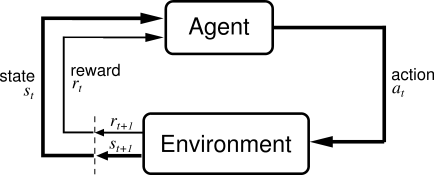
\includegraphics[scale=0.5]{img/I/figtmp7.png}
\centering
\captionsetup{justification=centering}
\caption{RL framework.}
\end{figure}

\textbf{Markov Decision Process} \\
In control theory, the decision making problem an RL agent faces is called an optimal control problem and is formalized as a Markov Decision Process (MDP), a discrete time stochastic control process used to model a decision making process where the controller interacts with a dynamic environment at each discrete timestep $t$ of a sequence. A MDP is defined by the tuple $<S,A,P,R>$, where $S$ is the set of states in the world, $A$ is the set of actions that the agent can take, $P(s_{t+1}|s_t,a_t)$ defines the transition dynamics, and $R(s_t,a_t,s_{t+1})$ is the reward function. A MDP is assumed to satisfy the Markov property, under which the environment's next state $s_{t+1}$ depends only on the current state $s_t$ and the action $a_t$ performed by the agent within this state. The MDP is thus memoryless, meaning that it doesn't rely on the history of past states to perform the next state transition. \\
The sequential decision making process is as follows, at each timestep $t$: 
\begin{enumerate}
    \setlength\itemsep{-0.5em}
    \item the agent makes an observation $x_t$ of  the environment $\varepsilon$ through input signals, i.e. sensors, and approximates the current state $s_t$ of the world with a state-observation pre-processing function $\phi_{s_t} = \phi(x_t) \sim s_t$, in the continuous state space $S$;
    \item the agent performs an action $a_t$ in response to the observed state $s_t$, chosen in the set of possible actions, the discrete action space $A=\{a_1,a_2,...,a_k\}$;
    \item the environment transitions from state $s_t$ to state $s_{t+1}$ as a result of action $a_t$, following the internal dynamics of $\varepsilon$, the finite probability transition matrix $P(s_{t+1}|s_t,a_t)$;
    \item the transition $(s_t,a_t,s_{t+1})$ yields an immediate reward $r_{t+1}$, the instantaneous return of taking action $a_t$ in state $s_t$ according to a reward function $R(s_t,a_t,s_{t+1})$.
\end{enumerate}
The goal of learning in a MDP is to find a policy $\pi(a,s) = p(a|s)$, a mapping from states to actions, that maximizes the long-term benefit, the sum of rewards that follow current time $t$.
As tasks are performed by completing a finite sequence of actions, a discount factor $\gamma \in \ ]0, 1[$ specifies how much immediate rewards are favored over distant rewards within a finite time horizon $T$. Within a finite horizon $T$, the MDP, although possibly arbitrarily large, is guaranteed to be finite. The future discounted reward at time $t$ is:
\[ 
\begin{split}
G_t &= \sum_{k=t}^{t+T} \gamma^{(k-t)} \cdot r_{k+1} = r_{t+1} + \gamma \cdot r_{t+2} + \gamma^2 \cdot r_{t+3} + \gamma^3 \cdot r_{t+4} + ... \\
&= r_{t+1} + \gamma \cdot (r_{t+2} + \gamma \cdot r_{t+3} + \gamma^2 \cdot r_{t+4} + ...) \\
&= r_{t+1} + \gamma \cdot G_{t+1}
\end{split}
\]

\textbf{Optimal action-value Q-function} \\
In environment $\varepsilon$, the transition $(s_t, a_t, s_{t+1}, r_{t+1})$ is not deterministic but stochastic, and the future discounted reward may differ between rollouts due to uncertainty over outcomes. Following the policy $\pi(a,s)$, the value function returns the expected discounted reward for being in the state $s_t$ over all possible trajectories:
\[ V_{\pi}(s) = \mathbf{E}_{\pi}[G_t|s_t=s,\pi] = \mathbf{E}_{\pi}[r_{t+1} + \gamma \cdot G_{t+1}|s_t=s,\pi] \]
With probabilistic state transition dynamics, the expected reward is: 
\[ r(s,a)=\mathbf{E}[r_t|s_{t-1}=s,a_{t-1}=a]=\sum_rr \sum_{s'}p(s',r|s,a) = \sum_{s',r}p(s',r|s,a) \cdot r \]
Thus, the value function becomes:
\[
\begin{split}
V_{\pi}(s) &= \sum_a\pi(a,s)\sum_{s',r}p(s',r|s,a)[r+\gamma \cdot \mathbf{E}_{\pi}[G_{t+1}|s_{t+1}=s']] \\
&= \sum_a\pi(a,s)\sum_{s',r}p(s',r|s,a)[r+\gamma \cdot V_{\pi}(s')]
\end{split}
\]
The recursion derived below is the Bellman equation, a recursive relationship between successive value functions in a MDP. It states that the value of a current state $s_t$ equals the value of the expected next state $s_{t+1}$, discounted by $\gamma$, and incremented by reward $r_{t+1}$.
\\

From the value function and with a fixed action $a_t$ at timestep $t$, the action-value Q-function can be expressed, the value of taking action $a_t$ in state $s_t$ following policy $\pi(a,s)$:
\[
\begin{split}
Q_{\pi}(s,a) &= \mathbf{E}_{\pi}[G_t|s_t=s,a_t=a,\pi] = \mathbf{E}_{\pi}[r_{t+1} + \gamma \cdot G_{t+1}|s_t=s,a_t=a,\pi] \\
&= \mathbf{E}_{\pi}[r_{t+1}+\gamma \cdot V_{\pi}(s_{t+1})|s_t=s,a_t=a,\pi] = \sum_{s',r}p(s',r|s,a)[r+\gamma \cdot V_{\pi}(s')] 
\end{split}
\]
The action-value Q-function assesses the quality of policies based on the value function and enables to rank the expected discounted rewards over states and actions. Thus, by maximizing the action-value Q-function, the agent derives the policy with the greatest expected return, the optimal policy $\pi^*(a,s)$. The  Bellman optimality equation defines the relationship between the optimal value function and the optimal action-value Q-function:
\[ 
\begin{split}
V_\pi^*(s) &= \max_a Q_\pi^*(s,a) \\
&= \max_a \mathbf{E}_{\pi}[r_{t+1}+\gamma \cdot V_{\pi}^*(s_{t+1})|s_t=s,a_t=a,\pi=\pi^*] = \max_a \sum_{s',r}p(s',r|s,a)[r+\gamma \cdot V_{\pi}^*(s')] \\
\end{split}
\]
Consequently, the optimal action-value Q-function is:
\[ Q_\pi^*(s,a) = \mathbf{E}_{\pi}[r_{t+1}+\gamma \cdot \max_{a'} Q_\pi^*(s_{t+1},a')|s_t=s,a_t=a,\pi=\pi^*] = \sum_{s',r}p(s',r|s,a)[r+\gamma \cdot \max_{a'} Q_\pi^*(s',a')] \]

\subsubsection{Q-learning algorithm} \label{basics}

\textbf{Q-learning and value-based RL} \\
Q-learning is a type of reinforcement learning that deals with learning indirectly the optimal policy $\pi^*(s,a)$ from the action-values of state-action pairs, in an unknown environment $\varepsilon$ with stochastic transitions $(s,a,s',r')$, mapping from a continuous state space $S$ to a discrete action space $A$, by optimizing the Q-function $Q_\pi(s,a)$. To do so, it approximates iteratively the optimal Q-function $Q_\pi^*(s,a)$ by selecting the action with the largest expected Q-value $arg\max_{a} Q_\pi(s,a)$ for the current state, learning the expected reward value of the state-action pair. For any finite MDP and given infinite learning time, exploration and exploitation, Q-learning can find an optimal policy: 
\[ \pi^*(s,a) = arg\max_{a}Q_\pi^*(s,a) \]
As the agent learns the optimal policy through the use of (action-) value functions, Q-learning belongs to the broader family of value-based reinforcement learning methods. \\

\textbf{Model-free learning and the explore-exploit trade-off dilemma} \\
Many optimization problems rely on model-based learning, where the complete model of the environment is known and classical dynamic programming techniques allow explicit planning by solving systems of equations. However, in many cases, the inner dynamics of the model is either unknown or too complex, and these methods become unfeasible. \
Contrariwise, Q-learning does not require prior knowledge of the environment, i.e. it is said to be model-free. Here, the probability distribution over transitions $p(s',r|s,a)$ is unknown, and is indirectly estimated by taking actions in a trial and error fashion. Thus, the learning task is completed by alternating between periods of exploration and exploitation. During exploration, the agent takes random actions, which are sub-optimal, in order to discover new states that haven't been visited so far. This allows the learning process to discover new regions of the state space, and avoid getting stuck in a sub-optimal local optimum. In fact, the function to be optimized is generally not convex, and consists of many local optima, which are optimal solutions within a neighboring set of candidate solutions, and the optimal local optimum being the global optimum, the optimal solution among all possible solutions. Exploration is meant to discover the widest range of local neighborhoods to gain a macroscopic knowledge over the shape of the function. Exploitation, on the other hand, optimizes the information acquired during exploration on a microscopic level, by finding the local optima within neighborhoods. Here, the agent is greedy to maximize the reward and takes the best known action, by highest Q-value. Therefore, it is during exploitation that the agent learns a solution to the optimization problem, whose quality is however subjected to the amount of previous exploration. This trade-off between exploration and exploitation is called the explore-exploit dilemma, and finding the adequate balance requires to  estimate the opportunity cost of greed. \\

\textbf{Off-policy learning and the epsilon-greedy policy} \\
While there is no ground rule to tackle the explore-exploit trade-off, Q-learning uses an action-selection policy known as epsilon-greedy, or $\epsilon$-greedy. This strategy is referred as off-policy, as the action-selection policy differs from the learned policy $\pi$ by including an epsilon $\epsilon$ threshold for random action selection. At each timestep, the agent will either explore and take a random action with probability $\epsilon$, or exploit and take the best known action for the given state with probability $1-\epsilon$ following the learned behavior policy $\pi$:
\[ 
\epsilon\text{-greedy policy: } a = 
    \begin{cases}
      arg \max_{a}Q_\pi(s,a) & \text{with probability } 1-\epsilon\\
      \text{rand a} \in A & \text{with probability } \epsilon
    \end{cases}
\]
There are many ways to define $\epsilon$, the most common being linear decay. At the beginning of learning, $\epsilon = 1$ as there is no knowledge of the environment to exploit. Then, as the need for exploitation decreases and exploitation becomes more important, $\epsilon$ is decayed linearly to a lower bound $\epsilon_{min}$ and over a period $\epsilon_{dec}$, following an interpolation function:
\[ 
\text{Linear decay: } \epsilon = 
    \begin{cases}
      t \cdot \frac{(\epsilon_{min}-1)}{\epsilon_{dec}} + 1 & \text{if } t < \epsilon_{dec}\\
      \epsilon_{min} > 0 & \text{else}
    \end{cases}
\]
The exploration probability must never end up null, as a continuous state space can never be fully explored by definition. Indeed, Q-learning converges in the long-term towards the best local optimum discovered, but is not guaranteed to discover the global optimum. \\

\textbf{Temporal difference learning and target update} \\
Q-learning learns the optimal Q-function by temporal difference, an iterative update of the Q-values over the difference between new and old estimates for a state-action pair. The mechanism used in temporal difference for creating new estimates from older samples is known as bootstrapping, and, since performed at each iteration, is said to be online. The temporal difference is the difference between a temporal difference target, an estimate of the Q-value for the next state computed from its expected optimal action-value, and the estimate of the Q-value for the current state. The temporal difference, weighted by a learning rate $\alpha$, is incremented to the current Q-value to update the Q-function:
\[ 
\begin{split}
Q_{\pi,t+1}(s_{t},a_{t})&= \mathbf{E}_{\pi}[r_{t+1}+\gamma \cdot \max_{a'} Q_{\pi,t}(s_{t+1},a')|s_t=s,a_t=a, \pi] \\
&=Q_{\pi,t}(s_{t},a_{t})+\alpha \cdot (r_{t+1}+\gamma \cdot \max_{a}Q_{\pi,t}(s_{t+1},a)-Q_{\pi,t}(s_{t},a_{t})) 
\end{split}
\]

\begin{figure}[h]
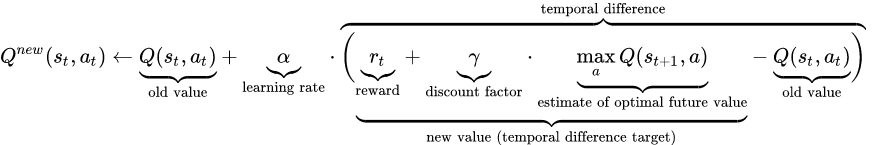
\includegraphics[width=\textwidth]{img/I/Selection_096.png}
\centering
\end{figure}

The learning rate parameter $\alpha$ controls the extent to which new estimates override old ones during the update. It metaphorically represents the speed at which the agent learns. Given infinite iterations of TD, Q-learning converges towards the optimal Q-function:

\[ Q_{\pi,t} \longrightarrow Q_{\pi,t}^*\ \text{, when}\ t \longrightarrow \infty \]

\textbf{Tabular Q-learning algorithm} \\
By the temporal difference definition, the optimization of the Q-function relies on its recursive property, derived from the Bellman optimality equation. A function approximator is therefore necessary to represent the Q-function in a way that is iteratively updateable.
In its original and simplest form, the Q-learning algorithm uses a table as a function approximator to store the Q-values of the Q-function, the Q-table. This Q-table is thus a $(|s|+1)$-dimensional matrix, with entries being the indices for the $|s|$-dimensional states and the $1$-dimensional actions, and the corresponding cells being the Q-values of the state-action pairs. Here, the continuous state space is divided into discrete bins of similar states for a discrete representation in the Q-table. The algorithm is as follows: 
For $E$ episodes, over the sequences from an initial to a terminal state, with total steps $t$, the agent observes the state $s$ and takes the action $a$ according to the $\epsilon$-greedy policy, and the model transitions to the next state $s'$, yielding reward $r'$. From the transition $(s,a,s',r')$, the agent updates, by temporal difference, the Q-value of the state-action pair in the Q-table.

\begin{algorithm}[H]
\small
\caption*{Tabular Q-learning algorithm}
\begin{algorithmic}
    \STATE Initialize step $t = 0$;
    \STATE Initialize $Q$-table $Q$ with $Q(s,a)=0$, $\forall s \in S$, $\forall a \in A$;
    \FOR{episode e = 1,E}
        \bindent
        \STATE Initialize sequence, observe initial state $s_t=\phi(x_t)$;
        \WHILE{$s_t$ not terminal}
            \bindent
            \STATE With probability $\epsilon$ select a random action $a_t \in A$
            \STATE otherwise select action $a_t = arg\max_{a}Q_{\pi,t}(s_t,a)$;
            \STATE Execute $a_t$ in  emulator $\varepsilon$ and observe reward $r_{t+1}$ and next state $s_{t+1}=\phi(x_{t+1})$;
            \STATE Update $Q_{\pi,t+1}(s_{t},a_{t}) =Q_{\pi,t}(s_{t},a_{t})+\alpha \cdot (r_{t+1}+\gamma \cdot \max_{a}Q_{\pi,t}(s_{t+1},a)-Q_{\pi,t}(s_{t},a_{t}))$;
            \STATE Decay $\epsilon$ with linear decay;
            \STATE Increment step $t = t + 1$;
            \eindent
        \ENDWHILE
        \eindent
    \ENDFOR
\end{algorithmic}
\end{algorithm}

\pagebreak
\subsection{Deep Q-learning} \label{basics}

In this second section of the first part, we present deep Q-learning, a variant of the aforementioned method combining the Q-learning algorithm with deep learning. Here, deep Q-learning, or DQN, does not refer to one algorithm, but a family of algorithms, among which the seven main ones are known as rainbow DQN [3] (Hessel et al., 2017). Four of those have been implemented as part of this internship, and are discussed here.

\subsubsection{DQN: Vanilla Deep Q-learning} \label{basics}

\textbf{From discrete to continuous state spaces} \\
For a long time, Q-learning has been restricted to its tabular version, and thus, to toy problems. In fact, the discretization of the state space and its storage in a table causes a major problem, i.e. the absence of generalization between states. In the Q-table, each Q-value is estimated separately, and must be updated many times for optimization. As the states represent combinations of multi-dimensional features, the MDP and the Q-table grow exponentially large with the state space, as every state encountered is virtually a new state. Thus, discrete representations of continuous problems are mostly impossible, the cost of exploring fine discrete states is immensely high, while the lack of details impedes learning when exploiting coarse discrete states. Several propositions have been considered for using Q-learning with continuous function approximators, such as genetic algorithms, support vector machines and shallow networks, however without significant improvements. In particular, neural networks seemed an appealing solution for approximating the Q-function, but it was found that non-linear approximators make Q-learning unstable and diverge in practice. Neural network based Q-learning was thought to be an insoluble problem for decades, until the rise of deep learning in the recent years allowed researchers at Google DeepMind to came up in 2015 with the deep Q-network, or DQN. \\

\textbf{Neural networks are continuous function approximators} \\
A neural network is a collection of interconnected artificial neurons, called perceptrons, approximating a function by mapping input data vectors to outputs. The simplest architecture for neural networks is the multi-layered perceptron (MLP), or simply artificial neural network (ANN), and is composed of $L$ successive layers of $s_l$ perceptrons. Each neuron from a layer $l$ is connected to all the neurons in the next layer $l+1$, and propagates an activation signal in the activation signal matrix $a$ through the network. The node $(l+1,i)$, the perceptron $i$ at layer $l+1$, acts like a simple mathematical unit and performs two operations, a dot product between the activation signals $a^{(l)}$ emitted by the previous layer and a set of weights $\Theta^{(l)}$ controlling the function mapping within the cross-layer connections and an additional bias unit, and a non-linear activation function $g^{(l)}$ on the resulting scalar $z$, then propagates the activation signal $a^{(l+1)}_i$ to the next layer: 
\[ a^{(l+1)}_i = g^{(l)}(z) \text{, with } z = \sum_{j=0}^{s_{l}} \Theta^{(l)}_{i,j} \cdot a^{(l)}_{j} \]
The input layer receives the raw input as activation, so that $a^{(1)} = X$. The activation function depends on the task and the depth in the network. In hidden layers, $g(l)$ is often the ReLU activation, or one of its variants, a rectifier linear unit, while the output layer can have $g(L-1)$ a sigmoid or tanh activation for binary classification (logistic regression), a softmax activation for multi-class classification, or no activation for raw output:
\[ ReLU(z) = \max(0,z) \text{, } sigmoid(z) = \frac{1}{1+e^{-z}}  \text{, } softmax(z)_i = \frac{e^{z_i}}{\sum_{j=1}^K e^{z_j}} \]
The whole propagation of a signal from the input layer through the output layer is the forward propagation, its result is a hypothesis $h_{\Theta}^{(m)} = a^{(L)}$ over the input training data $m$, and is performed over multiple inputs from a batch of $M$ training data. The neural network is a supervised learning tool, and uses labeled data to learn from the hypotheses. A loss function $L(y,h_{\Theta})$ measures the error between the batch of hypotheses $h_{\Theta}$ computed by forward propagation and the batch of corresponding real values $y$ of the outputs. The most common loss function is the L2-loss, the mean square error loss function (MSE):
\[ L(y,h_{\Theta}) = \frac{1}{2M}\sum_{m=1}^M (y^{(m)} - h_{\Theta}^{(m)})^2 \]
The goal of training a neural network is to minimize the loss function with respect to the weights, i.e. correcting the weights $\Theta_{i,j}^{(l)}$ in the network so that $L(y,h_{\Theta}) \rightarrow \min_{\Theta} L(y,h_{\Theta})$. An error term $\Delta_{i,j}^{(l)}$ is computed for all the weights by deriving the gradient of the loss function and the additional L2-norm $R(\Theta, \lambda)$ regularization term, over the weights $\Theta_{i,j}^{(l)}$:

\[ \Delta_{i,j}^{(l)} = \frac{\partial}{\partial \Theta_{i,j}^{(l)}} (L(y,h_{\Theta}) + R(\Theta, \lambda)) \text{, with } R(\Theta, \lambda) = \frac{\lambda}{2M}\sum_{l=1}^{L-1}\sum_{i=1}^{s_l}\sum_{j=1}^{s_{l+1}}(\Theta_{i,j}^{(l)})^2 \]

In practice, the gradient is computed by numerical approximations for each neuron, by propagating the error terms from the output layer to the input layer, the back propagation. It is during the back propagation that the weights $\Theta_{i,j}^{(l)}$ are corrected with an optimizer by the error $\Delta_{i,j}^{(l)}$ and a learning rate $\alpha$. This optimizer is the gradient descent algorithm:
\[ \Theta_{i,j}^{(l)} = \Theta_{i,j}^{(l)} - \alpha \cdot \Delta_{i,j}^{(l)} \]

Learning in a neural networks thus consists of approximating a function by mapping from input training data to output labels, through many forward and backward passes in layers of interconnected neurons, by measuring the average loss over batches of hypotheses and target values, and correcting the errors in the connection's weights with gradient descent. \\

\begin{SCfigure}[0][h]
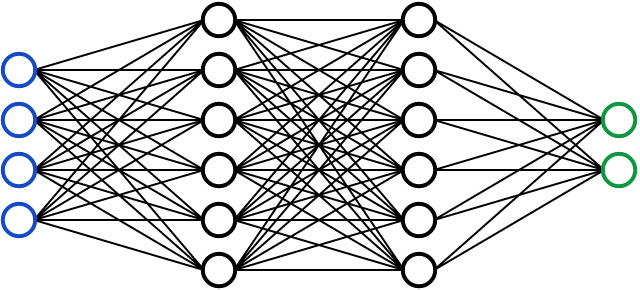
\includegraphics[scale=0.5]{img/I/Selection_098.png}
\centering
\caption{MLP.}
\end{SCfigure}

\textbf{Neural networks are unstable in Q-learning} \\
In Q-learning, neural networks are met with two primary issues that are inherent to RL. \\
(1) Successively correlated data; in supervised learning, data are inferred randomly from a prepared data set, and, while coming from the same data distribution, successive samples are not directly correlated. In Q-learning however, the data come from the observations of state transitions $(s,a,s',r')$ in a time sequence, and are thus highly successively correlated. This causes catastrophic forgetting, a phenomenon where the neural network over-fits to new experiences and unlearns old training, after having significantly changed the weights.
(2) Moving targets; in supervised learning, target values are labeled beforehand, and are therefore the exact and definitive values of optimal hypotheses. In Q-learning however, the targets are constructed dynamically by temporal difference from the Q-values. These estimates vary depending on the Q-function, that is iteratively updated through learning. While only the specific Q-value $Q_{\pi}(s,a)$ is updated at the given transition with a Q-table, a neural network updates all its weights at each back propagation pass, thus updating all the Q-values $Q_{\pi}(s,a)$ of the Q-function. Consequently, the estimated temporal difference targets are constantly changing, or moving, and any update can deeply alter the policy.
Because of (1) and (2), NN-based Q-learning has been known to be unstable and diverge. \\

\textbf{Deep Q-network, replay memory and target network} \\
In [4,5] (Mnih et al., 2015), the authors propose the deep Q-network algorithm (DQN), a convergent solution to Q-learning with a neural network as the Q-function approximator, later referred to as the vanilla DQN algorithm, i.e. as part of the rainbow DQN family. \\
Here, the Q-network $Q$ with weights $\Theta$ is a Q-function approximator such that $Q_{\pi}(s,a,\Theta) \approx Q^*_{\pi}(s,a)$, a neural network mapping from one state $s$ to all the Q-values $Q_{\pi}(s,a,\Theta), \forall a \in A$ for this state. The input layer is an $|s|$-dimensional vector, for the $|s|$ features of state $s$ in the continuous action space $S$, and the ouput layer is an $|A|$-dimensional vector, for the $|A|$ Q-values $Q_{\pi}(s,a,\Theta)$ of the $|A|$ possible actions $a$ in the discrete action space $A$, with $a = arg\max_a Q_{\pi}(s,a,\Theta)$ the optimal action to take following the optimal policy $\pi^*(s,a)$. \\
The two aforementioned problems causing the instability of neural networks as Q-function approximators are tackled with two novel key ideas, one respectively for each problem.
On the one hand, the replay memory addresses (1) the successively correlated data issue. The replay memory $D$ is a data buffer storing the $N$ last transitions experienced by the agent, $D = \{e_{t-1},e_{t-2},...,e_{t-N}\} \text{, with } e_t = (s_t,a_t,s_{t+1},r_{t+1})$. At each time step $t$, the agent stores the experienced transition $e_t$ in the replay memory, without updating the Q-network. It then draws uniformly at random $M$ past transitions from the replay memory, and performs an update of the Q-network by back propagation over this batch $U(D)$. Before the beginning of learning, the replay memory is filled with random transitions, i.e. transitions with only random actions taken, following an $\epsilon$-greedy policy with $\epsilon=1$. Hence, the bigger $N$ the size of the replay memory, the lower the correlation probability. \\
On the other hand, the target network addresses (2) the moving targets issue. The target $\hat{Q}$-network $\hat{Q}$ with weights $\Theta^-$ is a second neural network, copied from the online $Q$-network periodically every $C$ steps, such that $\Theta^-_t = \Theta_{\lfloor \frac{t}{C} \rfloor \cdot C}$, with $C$ the update target frequency. The target $\hat{Q}$-network is never updated by gradient optimization, and its weights $\Theta^-$ are held fixed and used for generating fixed temporal difference targets $y_t$ for the $C$ next updates of the online $Q$-network, introducing a delay that reduces divergence. \\
With the online $Q$-network $Q$, the replay memory $D$ and the target $\hat{Q}$-network $\hat{Q}$, DQN provides a stable model for approximating continuous Q-functions with neural networks. \\

\textbf{Vanilla DQN algorithm} \\
In the vanilla DQN algorithm, the $Q$-network replaces the Q-table as the Q-function approximator. The algorithm is as follows: The online $Q$-network $Q$ is initialized with random weights $\Theta_0$, and the target $\hat{Q}$-network $\hat{Q}$ is initialized with copied weights $\Theta^-_0=\Theta_0$. The replay memory buffer $D$ is initialized with capacity $N$, and  filled with $N_{min} \leq N$ random transitions, with random actions taken. For $E$ episodes, over the sequences from an initial to a terminal state, with total steps $t$, the agent observes the state $s_t=\phi(x_t)$, from observation $x_t$ and pre-processing function $\phi$, takes the action $a_t$ by Q-values $Q_{\pi,t}(s_t,a,\Theta_t)$ from forward propagation through the online $Q$-network $Q$ and according to the $\epsilon$-greedy policy, and the model transitions to the next state $s_{t+1}$, yielding reward $r_{t+1}$. The transition $(s_t,a_t,s_{t+1},r_{t+1})$ is stored in the replay memory buffer $D$, and a sample batch $U(D)$ of $M$ past transitions is drawn uniformly at random from the pool of stored experiences. The target $y^{(m)}_t$, the temporal difference target by forward propagation through the target $\hat{Q}$-network $\hat{Q}$, and the hypothesis $h_{\Theta,t}^{(m)}$, the Q-value by forward propagation through the online $Q$-network $Q$, are computed for each transition $(s,a,s',r')^{(m)}$ in the batch $U(D)$:
\[ y^{(m)}_t = r'^{(m)} + \gamma \cdot \max_{a'}Q_{\pi,t}(s'^{(m)},a',\Theta^-_t) \text{, } h_{\Theta,t}^{(m)} = Q_{\pi,t}(s^{(m)},a^{(m)},\Theta_t) \]
The online $Q$-network $Q$ is updated by back propagation with a gradient descent step on the gradient $\Delta_t$ derived from the MSE loss over the temporal differences $\delta^{(m)}_t = y^{(m)}_t - h_{\Theta,t}^{(m)}$:
\[
\begin{split}
 L_t(y_t,h_{\Theta,t}) &= \frac{1}{2M}\sum_{m=1}^M (y^{(m)}_t - h_{\Theta,t}^{(m)})^2 = L_t(\delta_t) = \frac{1}{2M}\sum_{m=1}^M (\delta_t^{(m)})^2 \\
 &= \frac{1}{2M}\sum_{m=1}^M (r'^{(m)} + \gamma \cdot \max_{a'}Q_{\pi,t}(s'^{(m)},a',\Theta^-_t) - Q_{\pi,t}(s^{(m)},a^{(m)},\Theta_t))^2
\end{split}
\]
Finally, the weights $\Theta^-$ of the target $\hat{Q}$-network $\hat{Q}$ are reset by copy of the weights $\Theta$ of the online $Q$-network $Q$ every $C$ steps, such that $\Theta^-_t = \Theta_t$ and $\hat{Q}_t = Q_t$ if $t \equiv 0 \pmod{C}$.

\begin{algorithm}[H]
\small
\caption*{Vanilla DQN algorithm}
\begin{algorithmic}
    \STATE Initialize step $t = 0$;
    \STATE Initialize the online $Q$-network $Q$ with random weights $\Theta_0$;
    \STATE Initialize the target $\hat{Q}$-network $\hat{Q}$ with weights $\Theta^-_0 = \Theta_0$;
    \STATE Initialize the replay memory buffer $D$ to capacity $N$
    \STATE with $Nmin$ random transitions $(s,\text{rand }a \in A,s',r')$;
    \FOR{episode e = 1:E}
        \bindent
        \STATE Initialize sequence, observe initial state $s_t=\phi(x_t)$;
        \WHILE{$s_t$ not terminal}
            \bindent
            \STATE With probability $\epsilon$ select a random action $a_t \in A$
            \STATE otherwise select action $a_t = arg\max_{a}Q_{\pi,t}(s_t,a,\Theta_t)$;
            \STATE Execute $a_t$ in emulator $\varepsilon$ and observe reward $r_{t+1}$ and next state $s_{t+1}=\phi(x_{t+1})$;
            \STATE Store transition $(s_t,a_t,s_{t+1},r_{t+1})$ in $D$;
            \STATE Sample random batch $U(D)$ of $M$ transitions $(s,a,s',r')^{(m)}$ in $D$;
            \FOR{m = 1:M}
                \bindent
                \STATE Set TD error $\delta^{(m)}_t = r'^{(m)} + \gamma \cdot \max_{a'}Q_{\pi,t}(s'^{(m)},a',\Theta^-_t) - Q_{\pi,t}(s^{(m)},a^{(m)},\Theta_t)$;
                \eindent
            \ENDFOR
            \STATE Perform a gradient descent step on MSE loss $L_t(\delta_t)$ w.r.t. $\Theta_t$,  with $\Delta_t$, $\alpha$;
            \IF{$t \equiv 0 \pmod{C}$}
                \bindent
                \STATE Reset target $\hat{Q}$-network $\hat{Q} = $ online $Q$-network $Q$, with $\Theta^-_t = \Theta_t$;
                \eindent
                \ENDIF
            \STATE Decay $\epsilon$ with linear decay;
            \STATE Increment step $t = t + 1$;
            \eindent
        \ENDWHILE
        \eindent
    \ENDFOR
\end{algorithmic}
\end{algorithm}

\textbf{Deep Q-learning converges, but is not optimized} \\
At this point, vanilla DQN provides a convergent model to approximate continuous Q-functions with neural networks in Q-learning. It is however not optimized, and extremely sample inefficient, requiring millions of time frames to optimize a Q-function, sometimes tens or hundreds of millions. The optimization of deep Q-learning algorithms has therefore become an active field of research in recent years, with many proposed improvements. \\
The rainbow DQN family lists six extensions that significantly improve specific aspects of the original vanilla DQN algorithm, towards a stabler and faster learning. Furthermore, these enhancements have been chosen to be mutually inclusive, and can be combined for better results, with each combination being virtually a new and functional DQN variant. \\
Three of these upgrades have been studied during this internship, and implemented together on top of the vanilla DQN to arrive at the algorithm used for the internship project.

\subsubsection{DDQN: Double Deep Q-learning} \label{basics}

\textbf{Overestimation in the TD target values} \\
DQN uses the temporal difference to build the target values $y_t$ from the target $\hat{Q}$-network $\hat{Q}$ in the loss function. However, in $max_{a'}Q_{\pi,t}(s',a',\Theta^-_t)$, the same $max$ operator both selects the action and evaluates the estimated Q-value for the temporal difference target. This maximization step is prone to favoring overestimated Q-values over underestimated ones, and results in overoptimistic Q-value estimates. DQN thus tends to develop unrealistically high value functions in the Q-function, thereby learning sub-optimal policies. \\

\textbf{Decoupling action selection and action evaluation} \\
In [6] (Hasselt et al., 2015), the authors present the double deep Q-network (DDQN) algorithm, effectively reducing overestimation by decoupling the selection of the action and the evaluation of the Q-value in the temporal difference target. In a two-step process, hence "double", the estimated optimal action is first selected by forward propagation through the online $Q$-network $Q$, and the corresponding estimated Q-value is then evaluated by forward propagation through the target $\hat{Q}$-network $\hat{Q}$. The TD target is thus re-written:
\[ y_t = r' + \gamma \cdot Q_{\pi,t}(s',arg\max_{a'}Q_{\pi,t}(s',a',\Theta_t),\Theta^-_t) \]

\subsubsection{3DQN: Dueling Double Deep Q-learning} \label{basics}

\textbf{Exploration efficiency and irrelevant actions} \\
In continuous state spaces, for many states, some actions do not affect the environment in any relevant way, and it is unnecessary to estimate the value of each action choice. In Q-learning however, the action-value function is an estimate of the value function over a specific action, and do not differentiate the value of being in a state and the advantage of taking an action from this state. The Q-network must thus estimate the state values for every state to choose an optimal action, assessing the inherent values of actions in respect to the Q-values only in retrospect. This causes DQN to be extremely sample inefficient, requiring long exploration times to derive good policies, i.e. tens of millions of samples. \\

\textbf{Decoupling value and advantage with the advantage function} \\
The dueling double DQN (3DQN) algorithm [7] (Wang et al., 2016), with its dueling network architecture, can learn which states are, and are not, valuable, without having to learn each action for each state, by decoupling the state values and the action advantages into value function $V_\pi(s)$ and advantage function $A_\pi(s,a)$. The dueling architecture learns a general state value that is shared across similar actions, leading to faster convergence and more efficient Q-functions. The Q-function measures the value of taking action $a$ being in state $s$, the V-function measures the value of being in state $s$, and the A-function measures the relative advantage of taking action $a$ deducing the value of being in state $s$:
\[ 
\begin{cases}
  Q_\pi(s,a) = V_\pi(s) + A_\pi(s,a) \\
  V_\pi(s) = \mathbf{E}_{\pi}[Q_\pi(s,a)|\pi] & \implies A_\pi(s,a) = Q_\pi(s,a) - V_\pi(s)\\
  \mathbf{E}_{\pi}[A_\pi(s,a)|\pi] = 0
\end{cases}
\]

\textbf{Dueling Q-network architecture} \\
The 3DQN algorithm introduces a novel neural network architecture specifically designed for value-based reinforcement learning, the dueling Q-network. A final hidden layer is added after the main network learning module, with weights $\Theta_t$, splitting the propagated signal into two streams for the value function and the advantage function. The $1$-dimensional value stream, with weights $\kappa_t$, estimates the scalar state value $V_{\pi,t}(s,\Theta_t,\kappa_t)$, and the $|A|$-dimensional advantage stream, with weights $\iota_t$, estimates the action advantage value vector $A_{\pi,t}(s,a,\Theta_t,\iota_t)$,  $\forall a \in A$. The value and advantage streams are combined to produce the Q-function $Q_{\pi,t}(s,a,\Theta_t,\iota_t,\kappa_t)$ in a special aggregation output layer, with:
\[ Q_{\pi,t}(s,a,\Theta_t,\iota_t,\kappa_t) = V_{\pi,t}(s,\Theta_t,\kappa_t) + (A_{\pi,t}(s,a,\Theta_t,\iota_t) - \frac{1}{|A|}\sum_{a'}A_{\pi,t}(s,a',\Theta_t,\iota_t)) \]

\begin{SCfigure}[0.1][h]
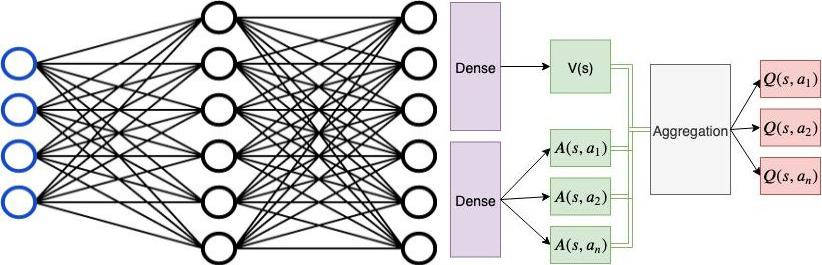
\includegraphics[scale=0.63]{img/I/Dueling-Q-architecture.jpg}
\centering
\caption{Dueling DQN.}
\end{SCfigure}

\subsubsection{Per3DQN: 3DQN with Prioritized Experience Replay} \label{basics}

\textbf{Exploitation efficiency and random transition sampling} \\
DQN uses an an experience replay memory buffer to store a pool of past experiences in the form of $(s,a,s',r')$ transitions, to solve the successively correlated data issue occurring when transitions are consumed online. The batches of transitions are however sampled over a random uniform probability distribution during Q-network updates, lacking a selection criterion to distinguish samples that could improve learning more than others. A selective sampling probability distribution, inferring samples proportionally to their estimated relative importance, would speed up exploitation, i.e. reduce sample inefficiency. \\

\textbf{Prioritized experience replay by TD error} \\
In [8] (Schaul et al., 2016), the authors present the prioritized experience replay (Per) algorithm, a novel proposition to more frequently replay transitions with high expected learning progress, i.e. the Per3DQN algorithm when combined with the 3DQN algorithm. \\
Here, prioritized sampling assigns a priority to transitions, so that samples with a higher priority are drawn more frequently from the replay memory buffer for training. Ideally, a utility function $f((s,a,s',r'))$ would return the exact priorities of transitions according to their usefulness in maximizing the cumulative reward. As such a function is unknown, the magnitude of the temporal difference error $|\delta|$ is a reasonable approximation to it, as the distance of the hypothesis from the target is what the Q-network aims to minimize. The absolute TD error thus transcribes how unexpected a transition was to the policy, i.e. how much the Q-function can learn from it. In the Per algorithm, a priority $p$ is computed from the absolute TD error $|\delta|$ and added to the transition $(s,a,s',r',p)$, which is stored in the prioritized replay memory composed of the replay memory and the sum tree. \\

\textbf{Efficient weighted sampling with the sum tree} \\
As the capacity $N$ of the replay memory $D$ is intended to be big to reduce correlation, the time complexity of frequently sampling transitions by priority value can rapidly grow. In Per, the prioritized transitions $(s,a,s',r',p)$ are split between the replay memory, a list-like collection of transitions $(s,a,s',r')$ with storage and access by indices in $O(1)$, and the sum tree, a separate binary tree collection of priorities $p$ and cumulative priorities, for efficient weighted sampling over the transitions in the replay memory by priority value. \\
In the sum tree, the leaf nodes correspond to the priorities $p_i$ of the transitions in the replay memory, and the parent of each node has a value equal to the sum of its two children, until the top node which has a value equal to the sum of all the leaf nodes. Hence, the sum tree is of size $2N - 1$ and zero-padded, with transition $i$ in the replay memory corresponding to leaf $N+i-1$ in the sum tree, and the cumulative sum of priorities $\sum_j p_j$ can be accessed in $O(1)$ at index 0. To extract the index $i$ of transition $(s,a,s',r')$ with priority $p_i$, the sum tree traverses the binary data structure from top to bottom, i.e.: \\
A uniform random value $v = U(0, \sum_j p_j)$ is sampled between 0 and the value of the top node, and three indices are initialized, namely the parent index $i_p=0$, the left child index $i_l=1$ and the right child index $i_r=2$, and the binary tree is then traversed iteratively. At each iteration, the left and right child indices are updated by $i_l=2i_p+1$ and $i_r=2i_p+2$. If $v$ is less or equal than the value of the left child node, $v \leq v_l$, then the left path is taken in the binary tree and the parent index is updated to the left child index, $i_p = i_l$. Else, $v$ is decremented by the value of the left child node, $v = v - v_l$, and the right path is taken in the binary tree and the parent index is updated to the right child index, $i_p = i_r$. If the left child index is greater than the size of the sum tree, $i_l \geq 2N - 1$, the parent index is equal to the leaf index, and the index $i$ of transition $(s,a,s',r')$ in the replay memory buffer sampled with priority $p_i$ is $i = i_p - N + 1$. The sum tree prioritized sampling operation is fast, completed in time complexity $O(\log n)$. Moreover, updating priorities in a sum tree is equally fast, as it only requires to propagate the difference bottom to top from the leaf node to the top node, from child node to parent node. Finally, the sum tree stores the maximum priority $p_{max}$ and minimum priority $p_{min}$ over all priorities at updates, so that they can be as well retrieved in $O(1)$. To summarize, the sum tree provides an optimized data structure for weighted sampling, with multiple fast operations over the priorities $p_i$. \\

\begin{SCfigure}[0.15][h]
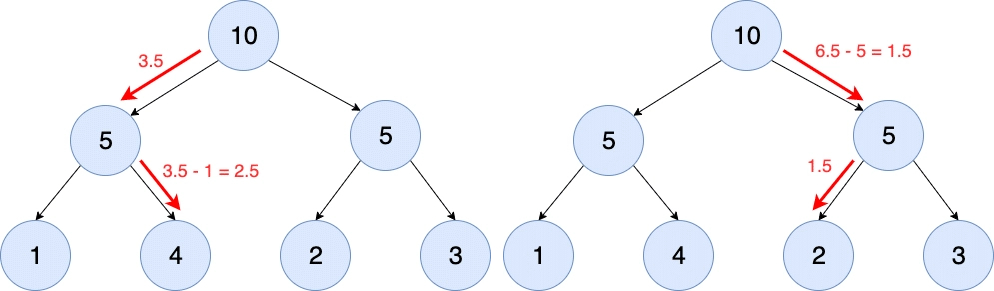
\includegraphics[scale=0.5]{img/I/Simple-SumTree-left-traverse.png}
\centering
\caption{Sum tree.}
\end{SCfigure}

\textbf{Priority update and distribution probability in the sum tree} \\
In DQN, the transitions are not consumed online, and the magnitude of the TD error $|\delta_t|$ for the current transition is unknown during exploration, it is thus stored with maximum priority $p_{max} \leq 1$ to assure that the transition is experienced at least once, i.e. the prioritized transition $(s_t,a_t,s_{t+1},r_{t+1}, p_{max})$. It is at Q-network gradient updates that the priorities $p_i^{(m)}$ are updated in the sum tree, the $M$ priorities of the prioritized transitions $(s,a,s',r',p_i)^{(m)}$ sampled in batch $P(D)$ with probability distribution $P(i)$ over the indices $i$ of the sum tree. The priorities $p_i^{(m)}$ are re-evaluated by absolute TD error, such that $p_i^{(m)}= min(|\delta^{(m)}_t| + \xi, 1)^{\eta}$, with $\xi \ll 1$, $\eta \in [0,1]$ and $p_i \in ]0,1]$. The $\eta$ coefficient determines the level of prioritization, with no prioritization for $\eta \rightarrow 0$, as all $p_i=1$, and full prioritization for $\eta \rightarrow 1$, as $p_i$ is fully dependant on the TD error magnitude. In practice, $\eta=0.6$ has been empirically found to work best. Furthermore, the sampling probability distribution over the indices $i$ in the sum tree is $P(i) = \frac{p_i}{\sum_j p_j} = \frac{p_i}{sum tree (0)}$.

\textbf{Correcting the gradient bias with importance sampling weights} \\
As the sampling probability distribution $P$ changes in an uncontrolled fashion, Per introduces a bias in learning that changes the solution that the estimates will converge to. This bias is corrected by using importance sampling (IS) weights $w_t$, to regularize the impact of over-sampled transitions on the Q-network parameters. Formally, IS weights compensate priority sampling with respect to the uniform distribution, so that prioritized transitions that are sampled as $(s,a,s',r',p) \sim P$, are experienced as $(s,a,s',r') \sim U$. The IS weights, computed over the priorities $p_i^{(m)}$ from the current batch, are $w_{t}^{(m)} = (N_t \cdot P(i))^{-\beta} / \max w_{t}$, with $Nt \leq N$ the current size of the replay memory buffer, $\beta$ a prioritization factor, and a normalization term for stability, i.e. the maximum weight for a priority in the sum tree, $\max w_{t} = (N_t \cdot \frac{p_{min}}{sum tree (0)})^{-\beta}$. As the training is highly unstable at the beginning of learning due to high randomness induced by exploration, the $\beta$ exponent controls the importance of prioritized sampling correction. In practice, $\beta$ is annealed linearly from $\beta \in [0.4,0.6]$ to $\beta=1$ over epsilon decay $\epsilon_{dec}$. The bias is then corrected by folding the IS weights $w_t$ with the TD errors $\delta_t$ in the loss function, re-adjusting the gradient $\Delta_t$ by the chain rule:
\[ L_t(\delta_t,w_t) = \frac{1}{2M}\sum_{m=1}^M w_{t}^{(m)} \cdot (\delta_t^{(m)})^2 \]

\begin{algorithm}[H]
\small
\caption*{Prioritized experience replay algorithm}
\begin{algorithmic}
    \STATE ...
    \STATE Initialize the replay memory buffer $D$ to capacity $N$
    \STATE with $Nmin$ random transitions $(s,\text{rand }a \in A,s',r')$;
    \STATE Initialize the sum tree to capacity $2N - 1$ with zero-padding;
    \FOR{step t = 1:T}
        \bindent
        \STATE ...
        \STATE Store prioritized transition $(s_t,a_t,s_{t+1},r_{t+1}, p_{max})$
        \STATE with $(s_t,a_t,s_{t+1},r_{t+1})$ in $D$ and $p_{max}$ in the sum tree;
        \STATE Sample prioritized batch $P(D)$ of $M$ transitions $(s,a,s',r',p_i)^{(m)}$, with $P(i) = \frac{p_i}{\sum_j p_j}$
        \STATE with $p_i^{(m)}$ in the sum tree and $(s,a,s',r')^{(m)}$ in $D$, with the sum tree sample algorithm;
        \FOR{m = 1:M}
            \bindent
            \STATE Set TD error $\delta^{(m)}_t = r'^{(m)} + \gamma \cdot \max_{a'}Q_{\pi,t}(s'^{(m)},a',\Theta^-_t) - Q_{\pi,t}(s^{(m)},a^{(m)},\Theta_t)$;
            \STATE Set priority $p_i^{(m)}= min(|\delta^{(m)}_t| + \xi, 1)^{\eta}$;
            \STATE Update priority $p_i^{(m)}$ in the sum tree, with the sum tree update algorithm;
            \STATE Set IS weight $w_{t}^{(m)} = (N_t \cdot P(i))^{-\beta} / \max w_{t} = (\frac{p_i^{(m)}}{p_{min}})^{-\beta}$;
            \eindent
        \ENDFOR
        \STATE Perform a gradient descent step on MSE loss $L_t(\delta_t,w_t)$ w.r.t. $\Theta_t$, with
        $\Delta_t$, $\alpha$;
        \STATE Anneal $\beta$ linearly;
        \STATE ...
    \ENDFOR
\end{algorithmic}
\end{algorithm}

\begin{algorithm}[H]
\small
\caption*{Sum tree sample algorithm, $O(\log n)$}
\begin{algorithmic}
    \STATE Initialize parent node index $i_p = 0$, left child node index $i_l = 1$, right child node index $i_r=2$;
    \STATE Initialize random uniform value $v = U(0, \sum_j p_j) = U(0, sumtree(0))$;
    \WHILE{$i_l < 2N-1$}
        \bindent
        \STATE Set $i_l = 2i_p+1$;
        \STATE Set $i_r = 2i_p+2$;
        \IF{$v > sumtree(i_l)$}
            \STATE Set $v = v - sumtree(i_l)$;
            \STATE Set $i_p = i_r$;
        \ELSE
            \STATE Set $i_p = i_l$; 
        \ENDIF
        \eindent
    \ENDWHILE
    \STATE Get transition $(s,a,s',r')$ with priority $p_i$ in $D$ at $D(i)$, with index $i=i_p - N + 1$;
\end{algorithmic}
\end{algorithm}

\begin{algorithm}[H]
\small
\caption*{Sum tree update algorithm, $O(\log n)$}
\begin{algorithmic}
    \STATE Initialize propagation index with leaf node index $i_t = i+N-1$;
    \STATE Set propagation difference value $d = p_i - sumtree(i_t)$;
    \STATE Update $p_{max} = max(p_i,p_{max})$, $p_{min} = min(p_i,p_{min})$;
    \STATE Update priority value $sumtree(i_t) = p_i$;
    \WHILE{$i_t$ not $0$}
        \bindent
        \STATE Set $i_t = \lfloor(i_t - 1) / 2\rfloor$;
        \STATE Propagate difference $sumtree(i_t) = sumtree(i_t) + d$;
        \eindent
    \ENDWHILE
\end{algorithmic}
\end{algorithm}

\textbf{Towards state of the art with rainbow DQN} \\
The rainbow DQN framework lists three additional extensions to the vanilla DQN algorithm, apart from the three discussed here. (1) Noisy DQN learns to ignore perturbations in the training data by incorporating a noisy stream to the Q-network. (2) N-step DQN accumulates a multi-step target to learn rewards over sequences of n steps, rather than immediate rewards. (3) Distributional DQN learns distributional returns instead of expected ones by minimizing the Kullback–Leibler divergence over online and target distributions. \\
When combined; i.e. vanilla DQN with double TD target, dueling NN architecture, prioritized experience replay, noisy stream, n-step reward and distributional return; the resulting algorithm is the state of the art for deep Q-learning, the rainbow DQN algorithm. 

\pagebreak
\subsection{DQN in customized environments}

In this third section of the first part, we present frameworQ, a python framework for applying deep Q-learning algorithms in customized environments, developed during the first half of the internship. DQN algorithms are notoriously difficult to implement and debug, and reproducibility is a major issue in the field of deep reinforcement learning. With frameworQ, we aim at providing a ready-to-use and flexible baseline of DQN algorithms and environment wrappers to facilitate research, allowing to generate results faster by putting the focus on designing environments and their action/observation/reward functions, and hyper-parameter tuning. We first present the framework architecture and implementation, then describe global guidelines to tune hyper-parameters in practice, and finally demonstrate the proof of concept with two toy environments. The framework was used as a base code for the internship project in the second half of the internship. frameworQ is available at: \textbf{\url{https://github.com/romainducrocq/frameworQ}}.

\subsubsection{Presentation of frameworQ} \label{basics}

\textbf{Overview} \\
frameworQ is a python framework developed to facilitate research applications based on deep Q-learning algorithms. It provides a ready-to-use and fully abstracted DQN code baseline, and additional features and tools, in a standalone package, and entry scripts for training, testing, visualizing and comparing agents, with flexible command line control. It allows users to focus solely on creating customized environments, in an environment dedicated package, following a simple MVC prepared structure. As such, we intent to minimize the implementation effort and make deep Q-learning research more accessible. \\

\textbf{Global architecture} \\
frameworQ runs under a python virtual environment \texttt{venv/}, and an installation script is provided to build frameworQ and its dependencies, at \texttt{bin/make.sh}. The DQN code baseline is encapsulated in the \texttt{dqn/} package, and requires no modification, i.e. it is intended to be fully abstracted from the user. The customized environment is to be created in the \texttt{env/} package, and splitted into model, view and controller within structured templates, which consists of the only code to adapt. Three main scripts are used as entry points to the programs, \texttt{train.py} to train an agent with a set of hyper-parameters, \texttt{observe.py} to deploy a trained neural network for testing, and \texttt{play.py} to load the environment with non-DQN controllers for comparison. These can be launched from command lines with arguments or from shell scripts in \texttt{bin/}, as well as additional tools for visualizing learning curves and evaluation metrics. Two more folders \texttt{save/} and \texttt{logs/} respectively store trained models and log files, which are singled into \texttt{train/} and \texttt{test/}.

\pagebreak

\textbf{DQN baseline in \texttt{dqn/}} \\
The \texttt{dqn/} package groups the ready-to-use DQN baseline code, and implements the four algorithms presented in section 2; i.e. DQN, DDQN, 3DQN and Per3DQN; and further improvements presented hereafter, fully abstracted from the user. It is based on \texttt{Pytorch}, a heavily optimized machine learning library for tensor operations in neural networks, on both CPU and GPU. \texttt{agent.py} implements the agent, with the TD update for the four algorithms, the action-selection policy, the transition to tensor conversion and the training logs. These logs, i.e. the averaged rewards and durations over the last 100 episodes, are written to \texttt{.tfevents} log files in the \texttt{logs/train/} folder every $f_l$ timesteps, a log frequency defaulted to 1000 timesteps, with \texttt{Tensorboard}, a toolkit to visualize learning curves over training and evaluate agents. \texttt{network.py} implements the neural networks for online and target $Q$-networks, with both simple and dueling architectures, and dynamic model saving and loading. The model, i.e. the weights $\Theta_t(, \iota_t, \kappa_t)$ of the online $Q$-network $Q$ at timestep $t$, are saved to binary \texttt{.pack} files in the \texttt{save/} folder every $f_s$ timesteps, a save frequency defaulted to 10000 timesteps, with \texttt{msgpack}, an efficient object serialization library for \texttt{numpy} arrays. \texttt{replay\_memory.py} implements the replay memory data buffer, with both uniform and prioritized transition sampling. \texttt{env\_wrap.py} wraps the customized environment in \texttt{OpenAi Gym}, a reinforcement learning toolkit for simulated environments with many features, and writes the test logs, i.e. additional transition information defined by the user, as \texttt{.csv} files in the \texttt{/logs/test/} folder for further analysis. \texttt{env\_make.py} instantiates the customized environment and implements multi-processing training with \texttt{SubprocVecEnv}, a vectorization tool for training multiple environments in parallel over sub-processes. Finally, the \texttt{utils/} folder contains the implementation of the sum tree, a meta-class definition and all the dependencies of the aforementioned tools. 
\\

\textbf{Customized environment in \texttt{env/}} \\
The \texttt{env/} package contains a simple model, view, controller template structure for the creation of customized environments, and a hyper-parameter configuration file, and is the only code to be adapted in frameworQ. The model of the environment, i.e. all the object classes and additional resources, must be defined in the \texttt{custom\_env/} folder. The controller of the environment must be wrapped in \texttt{dqn\_env.py} in a DQN oriented structure, with action space size $|A|$ and state feature size $|s|$, observation pre-processing function $\phi$, reward function $R$, terminal state function, environment reset function and transition dynamics function $P$ for one timestep $t$, and optionally additional transition log information, and logic functions for the view only. A view can be optionally set for the environment in \texttt{view.py}, with either a template provided in \texttt{Pyglet}, a python interface for the graphics library \texttt{OpenGl}, or an empty wrapper for customized views. The view is activated only at deployment, and not during training for resource optimization, and can be disabled fully. The hyper-parameter configuration file \texttt{dqn\_config} contains all the hyper-parameters of the DQN algorithms to be tuned, as well as the neural network architecture, the loss function and the gradient optimizer. Default values for all those are provided as a starting point for tuning. A full guide for building customized environments can be found in \texttt{doc/}. \\

\textbf{Code modularity and flexible command control} \\
frameworQ is developed in a modular object-oriented paradigm, with extensive functional decomposition and class inheritance, in order to be easily maintained and updated. Moreover, it is designed such that DQN algorithms can be added towards full rainbow DQN. The main program scripts \texttt{train.py}, \texttt{observe.py} and \texttt{play.py} allow abundant line command control for flexible use, with the complete list of arguments detailed again in \texttt{doc/}.

\subsubsection{Further optimization, Per3DQN+} \label{basics}

\textbf{Optimized implementation} \\
Additionnaly to the four algorithms presented in section 2; i.e. DQN, DDQN, 3DQN and Per3DQN; frameworQ incorporates further optimization features that have been picked from the recent ML / RL literature, in an effort to maximize learning speed and stability:
\begin{itemize}
\setlength\itemsep{-0.5em}
  \item \textbf{MinMax scaling}: Neural networks are very sensitive to the range of input features, and  normalization in $[-1,1]$ both accelerates learning and reduces the risk for exploding gradients. In supervised learning, where the data distribution is known, it is common practice to normalize by Z-score. However, in reinforcement learning, as the data is online, we prefer to include min-max scaling in $[0, 1]$ in the observation pre-processing function $\phi$. If the bounds for input features are unknown, data are scaled by the minimum and maximum values encountered at that time of training:
  \[ MinMax(x) = \frac{x - x_{max}}{x_{min} - x_{max}}, Z-score(x) = \frac{x - \mu}{\sigma} \]
  \item \textbf{Exponential decay}: The explore-exploit trade-off has been empirically found to have a better balance with exponential decay, with $\epsilon$-decay slowing down over time:
  \[ 
  \text{Exponential decay: } \epsilon = 
  \begin{cases}
      \exp(t \cdot \frac{\log(\epsilon_{min})}{\epsilon_{dec}}) & \text{if } t < \epsilon_{dec}\\
      \epsilon_{min} > 0 & \text{else}
  \end{cases}
  \]
  \item \textbf{ELU activation}: ReLU non-linearities don't handle negative inputs and are subject to vanishing gradients, causing the dying ReLU problem. The exponential linear unit activation (ELU) is a similar identity function and a strong alternative to ReLU that can produce smooth small negative outputs in $[-1,0]$ for negative values:
  \[
  ELU(z)=
  \begin{cases}
      z & \text{if } z > 0 \\
      e^z - 1 & \text{else}
  \end{cases}
  \]
  \item \textbf{Huber loss}: Deep Q-learning is extremely sensitive to outliers in the training data, and the MSE loss, while efficient, introduces instability with the square term. The Huber loss provides a robust substitute, by alternating between the mean square error L2-loss for small values of the TD error magnitude and the mean absolute error L1-loss for larger values, a stabilization method called gradient error clipping:
  \[ 
  \text{Huber loss: } L_t(\delta_t, w_t) = \frac{1}{2M}\sum_{m=1}^M w_t^{(m)} \cdot
  \begin{cases}
      \text{MSE L2-Loss: }(\delta_t^{(m)})^2 & \text{if } |\delta_t^{(m)}| < 1 \\
      \text{MAE L1-Loss: }2 \cdot |\delta_t^{(m)}| - 1 & \text{else}
  \end{cases}
  \]
  \item \textbf{Adam optimizer}: Gradient descent faces limited performances in deep neural networks, due to slow convergence. The adaptive moment estimation optimizer (Adam) [9] (Kingma, Ba, 2017), speeds up parameter optimization by correcting the gradient update with a momentum correction term $v_t$ and a root mean square propagation term $s_t$ (RMSprop), with learning rate $\alpha$ and coefficients $\beta_1$, $\beta_2$ and $\epsilon$:
  \[ 
  \text{Adam optimizer: } 
  \begin{cases}
      v_t = \frac{\beta_1 \cdot v_{t-1} + (1 - \beta_1) \cdot \Delta_{i,j}^{(l)}}{1-\beta_1^t} & \text{with } v_0=0, \beta_1 = 0.9\\
      s_t = \frac{\beta_2 \cdot s_{t-1} + (1 - \beta_2) \cdot \Delta_{i,j}^{2(l)}}{1-\beta_2^t} & \text{with } s_0=0, \beta_2 = 0.999\\
      \Theta_{i,j}^{(l)} = \Theta_{i,j}^{(l)} - \alpha \cdot \frac{v_t}{\sqrt{s_t} + \epsilon} & \text{with } \epsilon = \num{1e-8}\\
  \end{cases}
  \]
  \item \textbf{Polyak update}: The target $\hat{Q}$-network $\hat{Q}$ is updated by hard copy of the $Q$-network $Q$ every $C$ steps, the target update frequency. This causes learning to be unstable for a small time interval after copies, when the correlation between TD targets and online Q-values is still strong, and makes the Q-function sometimes diverge locally. The Polyak soft update [10] (Lillicrap et al., 2019) smoothes the updates by updating the weights $\Theta_t^-$ of the target $\hat{Q}$-network $\hat{Q}$ by a very small rate $\tau$ of the weights $\Theta_t$ of the $Q$-network $Q$ at each time step $t$. Thus, $\hat{Q}$ always converges towards $Q$, but with a sufficient delay for decorrelation between TD targets and online Q-values:
  \[ \Theta^-_t = (1-\tau) \cdot \Theta^-_t + \tau \cdot \Theta_t \text{, with } \tau \ll 1\]
  \item \textbf{Action repeat}: The time steps $t$ do not have to coincide with the real clock rate of the environment $\varepsilon$. Moreover, knowing that difficulty of performing optimal sequences of actions rises with the horizon $T$, learning can strongly benefit from adjusting the action interval to an optimal decision frequency for the task. At each time step $t$, the action $a_t$ is repeated $k$ times in the environment $\varepsilon$, and the reward $r_{t+1}$ is obtained by accumulating the intermediate rewards, such that $r_{t+1} = \sum_k r_k$.
  \item \textbf{Time limit}: In early phases of learning, it often happens that the best known policy is simply to avoid terminal states, associated with penalties. The agent thus starves, and selects sub-optimal actions that, while performing poorly, extend the episode. A time limit is set on episodes to avoid cases of starving, i.e. early stopping.
\end{itemize}

\pagebreak

\textbf{Combining everything with Per3DQN+} \\
In frameworQ, by combining the four algorithms presented in section 2; i.e. vanilla, double, dueling and Per DQN; and the additional improvements presented hereinabove, we obtain the algorithm used for the internship project, presented later on in the second part. We call this algorithm the Per3DQN+ algorithm for simplicity, and it is as follows:

\begin{algorithm}[H]
\small
\caption*{Per3DQN+ algorithm}
\begin{algorithmic}
    \STATE Initialize step $t = 0$;
    \STATE Initialize the online dueling $Q$-network $Q$ with random weights $\vartheta_0 = (\Theta_0, \iota_0,\kappa_0)$;
    \STATE Initialize the target dueling $\hat{Q}$-network $\hat{Q}$ with weights $\vartheta^-_0 =  (\Theta^-_0, \iota^-_0,\kappa^-_0) = \vartheta_0$;
    \STATE Initialize the replay memory buffer $D$ to capacity $N$
    \STATE with $Nmin$ random transitions $(s,\text{rand }a \in A,s',r')$;
    \STATE Initialize the sum tree to capacity $2N - 1$ with zero-padding;
    \FOR{episode e = 1:E}
        \bindent
        \STATE Initialize sequence, observe initial state $s_t=\phi(x_t) \sim MinMax$;
        \WHILE{$s_t$ not terminal \textbf{and} time not limit}
            \bindent
            \STATE With probability $\epsilon$ select a random action $a_t \in A$
            \STATE otherwise select action $a_t = arg\max_{a}Q_{\pi,t}(s_t,a,\vartheta_t)$;
            \FOR{repeat k=1:K}
                \bindent
                Execute $a_t$ in emulator $\varepsilon$ and accumulate reward $\sum_k r_k$;
                \eindent
            \ENDFOR
            \STATE Observe reward $r_{t+1}$ and next state $s_{t+1}=\phi(x_{t+1}) \sim MinMax$;
            \STATE Store prioritized transition $(s_t,a_t,s_{t+1},r_{t+1}, p_{max})$
            \STATE with $(s_t,a_t,s_{t+1},r_{t+1})$ in $D$ and $p_{max}$ in the sum tree;
            \STATE Sample prioritized batch $P(D)$ of $M$ transitions $(s,a,s',r',p_i)^{(m)}$, with $P(i) = \frac{p_i}{\sum_j p_j}$
            \STATE with $p_i^{(m)}$ in the sum tree and $(s,a,s',r')^{(m)}$ in $D$, with the sum tree sample algorithm;
            \FOR{m = 1:M}
                \bindent
                \STATE Set double TD error $\delta^{(m)}_t = r'^{(m)} + \gamma \cdot Q_{\pi,t}(s'^{(m)},arg\max_{a'}Q_{\pi,t}(s'^{(m)},a',\vartheta_t),\vartheta^-_t)$ \\ \;\;\;\;\;\;\;\;\;\;\;\;\;\;\;\;\;\;\;\;\;\;\;\;\;\;\;\;\;\;\;\;\;\;\;\;\;\;\;\;\;\;\;
                $-$ $Q_{\pi,t}(s^{(m)},a^{(m)},\vartheta_t)$;
                \STATE Set priority $p_i^{(m)}= min(|\delta^{(m)}_t| + \xi, 1)^{\eta}$;
                \STATE Update priority $p_i^{(m)}$ in the sum tree, with the sum tree update algorithm;
                \STATE Set IS weight $w_{t}^{(m)} = (N_t \cdot P(i))^{-\beta} / \max w_{t} = (\frac{p_i^{(m)}}{p_{min}})^{-\beta}$;
                \eindent
            \ENDFOR
            \STATE Perform an Adam optimizer step on Huber loss $L_t(\delta_t,w_t)$ w.r.t. $\vartheta_t$, with $\Delta_t$, $\alpha$;
            \STATE Soft update target $\hat{Q}$-network $\hat{Q}$ with Polyak update, with $\vartheta^-_t = (1-\tau) \cdot \vartheta^-_t + \tau \cdot \vartheta_t$;
            \STATE Save model every $f_s$ steps, log metrics every $f_l$ steps;
            \STATE Decay $\epsilon$ with exponential decay, anneal $\beta$ linearly;
            \STATE Increment step $t = t + 1$;
            \eindent
        \ENDWHILE
        \eindent
    \ENDFOR
\end{algorithmic}
\end{algorithm}

\subsubsection{Hyper-parameter tuning in practice} \label{basics}

\textbf{Hyper-parameter tuning in RL} \\
Machine learning algorithms include control parameters that can not be learned but must be hand-picked, i.e. the set of hyper-parameters. In reinforcement learning especially, their impact on learning is major, and they have to be tuned carefully. There is no established method to automatically find the optimal values, and the most effective tuning process remains to perform a grid search over the hyper-parameters, by changing one parameter at a time and observing the effects on the cumulative reward. This operation must be repeated several times, as seeds can not be used in training due to the randomness of environments themselves, making tuning come at a high computational cost. Thus, it is best practice to tune hyper-parameters by impact on learning and within ranges of common values, while keeping track of training progress with rewards and evaluation metrics. \\

\textbf{Practical guidelines for hyper-parameter tuning} \\
We propose here a global scheme for hyper-parameter tuning, by order and value ranges:
\begin{enumerate}
    \setlength\itemsep{-0.5em}
    \item \textbf{Learning rate $\alpha \in ]0, 1[$}: The learning rate is by far the most impactful hyper-parameter. It controls the step size in gradient updates during loss minimization, with bigger Q-network weight updates when $\alpha \rightarrow 1$, and thus faster learning. However, the Q-function diverges for steps too big, and $\alpha$ must be set to the highest value for which training converges. In practice, it is advised to set $\alpha$ to an order of magnitude less than this highest value, as Q-learning is a non-stationary problem and requires lower update steps towards the end of training. The learning rate is to be tested on a logarithmic scale, with typical values being in $\{\num{1e-1},\num{1e-2},\num{1e-3},\num{1e-4},\num{1e-5}\}$. In broad, the more complex the NN, the lower $\alpha$.
    \item \textbf{Discount factor $\gamma \in ]0, 1[$}: The agent is myopic and favors immediate reward for $\gamma \rightarrow 0$, while it is far-sighted for $\gamma \rightarrow 1$. The discount factor should be high enough to take into account distant future, but a too high value will cause instabilities. A good approach to approximate $\gamma$ is to estimate the number of actions needed to perform a task, i.e. the horizon $T$, and compute: $\gamma = 1 - \frac{1}{T}$. In practice, $0.9 \ (T = 10) \leq \gamma \leq 0.99 \ (T = 100)$, with common values in $\{0.9, 0.95, 0.98, 0.99\}$.
    \item \textbf{Neural network width and depth}: For MLPs, a rule of thumb is to set the number of neurons per layer $n$ to the greatest power of two that is smaller than ten times the dimension of the input observation, such that $n = 2^x \leq 10 \cdot |s| < 2^{x+1}$. As for the depth of the NN, a perfectly tuned MLP with two hidden layers can map any continuous function after infinite optimization. Hence, a MLP can be first tested with two hidden layers, and adding layers until no further improvement is visible.
    \item \textbf{Exploration parameters $\epsilon_{min} \in ]0, 1[$ and $\epsilon_{dec}$}: The minimum exploration rate $\epsilon_{min}$ during exploitation must not exceed a rate of sub-optimal random actions for which the task will probably not be completed, and is generally in $\{0.1, 0.05, 0.01\}$. The duration over which the exploration rate is decayed $\epsilon_{min}$ is usually set to half of the training time, or the full training time. It can be first tested for 1M timesteps, and progressively increased by steps of 1M until no further improvement is visible.
    \item \textbf{Target update parameters $C$ and $\tau \ll 1$}: For hard target $\hat{Q}$-network updates, the update target frequency $C$ must be high enough to stabilize TD targets and decorrelate them from Q-values, with $C$ often found in $\{10000,30000,50000\}$. For soft Polyak updates, a $\tau$ rate of $\num{1e-3}$ appears to work indiscriminately for all tasks.
    \item \textbf{Replay memory capacity $N$ and initial size $N_{min}$}: The replay memory buffer must have the biggest capacity possible to decorrelate successively experienced data. While $N$ should be infinite in theory, a capacity $N$ of 1M transitions is acceptable in practice. The initial size $N_{min}$ in $\{\frac{N}{10},\frac{N}{5},\frac{N}{2},N\}$, depends on the initialization cost.
    \item \textbf{Repeat parameter $k$}: E.g., it is detrimental to learning to have an agent try to predict hundreds of actions per second for tasks intended for humans, which can at best take ten actions per second for experts, but perform tasks over several seconds. For such tasks, $4 \leq k \leq 16$ can greatly accelerate learning and enhance performance.
    \item \textbf{Batch size $M$}: The batch size, the number of $M$ transitions that are sampled for computing the loss at $Q$-network updates, can be tuned, yet with only little impact, as a power of two for computational efficiency, commonly within $16 \leq M \leq 512$. 
\end{enumerate}

\subsubsection{Demo: two customized toy environments} \label{basics}

\textbf{Proof of concept with two customized toy environments} \\
As a proof of concept, we demonstrate frameworQ with two customized toy environments. Here, the DQN code is strictly identical between the two examples, and only the environment model package, the DQN controller, the Pyglet view and the hyper-parameter configuration file are adapted. For both examples, we arrive at expert level performances. \\

\textbf{Customized toy environment 1: Racing Car} \\
In the first customized toy environment, the agent controls a car racing around a track. At the beginning of an episode, a randomly generated track is created and the car is spawned over a randomly positioned starting line. When the car hits a border, the episode is terminated and the environment is reset with a new generated track. The track generation follows a Gaussian law over randomly generated polygons, so that the agent never encounters two times the same track. The agent observes 37 features; the speed of the car and the distance to the nearest border in 36 directions. The agent can choose between 5 actions; accelerating, decelerating, turning right, turning left and doing nothing. 100 reward gates are spaced linearly around the track, and the agent gets a reward of +1 if the car passes the next gate, and no reward otherwise. The tuned hyper-parameters are $\alpha=\num{5e-5}$ with Adam optimizer and Huber loss, $\gamma=0.99$, $\epsilon_{min}=0.01$, $\epsilon_{dec}=10$M with exponential decay, $N=1$M, $N_{min}=1$M, $\tau=\num{1e-3}$ with soft Polyak update, actions are repeated over $k=8$ frames, $M=32$, and a time limit of $5000$ timesteps is set per episode. \\ The neural network is a MLP with two hidden layers of $256$ neurons each and ELU activations, and the agent was trained over 18M timesteps with the Per3DQN+ algorithm.
The agent attains expert level performances, surpassing by far an average human player. \\
It achieves an average of five loops around the track at high speed before either time limit early stopping for most of the tracks or hitting a border for some of the harder tracks. Due to random track generation and game physics, some turns are overly difficult, and the agent has learned to turn around in such cases, developing an effective survival strategy. \\
It is available at: \textbf{\url{https://github.com/romainducrocq/initial-DQN}}. \\

\begin{figure}[h]
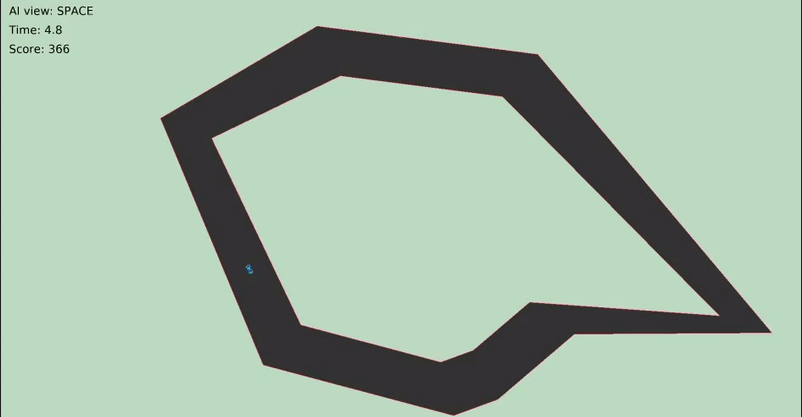
\includegraphics[scale=0.5]{img/I/Selection_107.png}
\centering
\end{figure}

\begin{figure}[h]
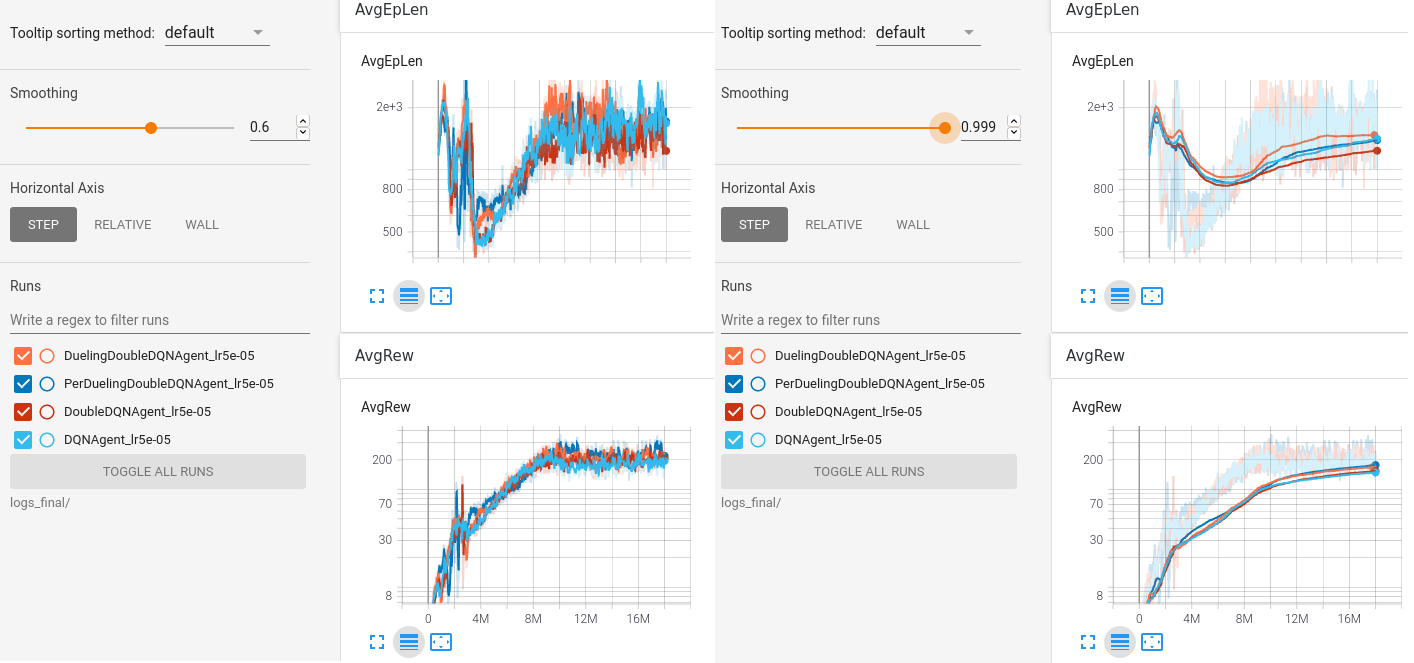
\includegraphics[width=\textwidth]{img/I/Selection_100.png}
\centering
\captionsetup{justification=centering}
\caption{Demo, customized environment 1; (1) visual, (2) learning curves.}
\end{figure}

\pagebreak

\textbf{Customized toy environment 2: Flappy Bird} \\
In the second customized toy environment, the agent controls a game character in a clone of the famous "Flappy Bird" game. The character, represented here by a swimming monkey rather than a flying bird, is in the left side of the screen, with a fixed horizontal position. Pipes covering the full height of the screen are generated at regular intervals at the right end of the screen, and traverse the screen from side to side. The monkey can only swim or sink over the vertical axis and must avoid the pipes by passing through a small gap placed at a random height. When the monkey hits a pipe, the episode is terminated and the environment is reset. The agent observes 3 features; the horizontal distance to the next pipe, the vertical distance to the middle of the gap in the next pipe, and whether it is above or under the middle of this gap on the vertical axis. The agent can choose between 2 actions; swimming to go up and doing nothing to sink down. At each timestep, the agent is punished by the squared distance to the horizontal line passing by the middle of the gap in the next pipe, or is not punished after passing a pipe. The tuned hyper-parameters are $\alpha=\num{1e-3}$ with Adam optimizer and Huber loss, $\gamma=0.9$, $\epsilon_{min}=0.01$, $\epsilon_{dec}=2$M with exponential decay, $N=1$M, $N_{min}=1$M, $\tau=\num{1e-3}$ with soft Polyak update, actions are repeated over $k=5$ frames, $M=32$, and a time limit of $5000$ timesteps is set per episode. The neural network is a MLP with two hidden layers of $16$ neurons each and ELU activations, and the agent was trained over 9M timesteps with the Per3DQN+ algorithm. The agent attains optimal performances, beating the game fully. \\
During deployment, it was consistently stopped by time limit early stopping without hitting a pipe, and was therefore tested without time limit. After eight hours, we stopped the game after the agent had passed more than 15000 pipes without loosing a single time.
It is available at: \textbf{\url{https://github.com/romainducrocq/flappy-seamonkai}}.

\begin{figure}[h]
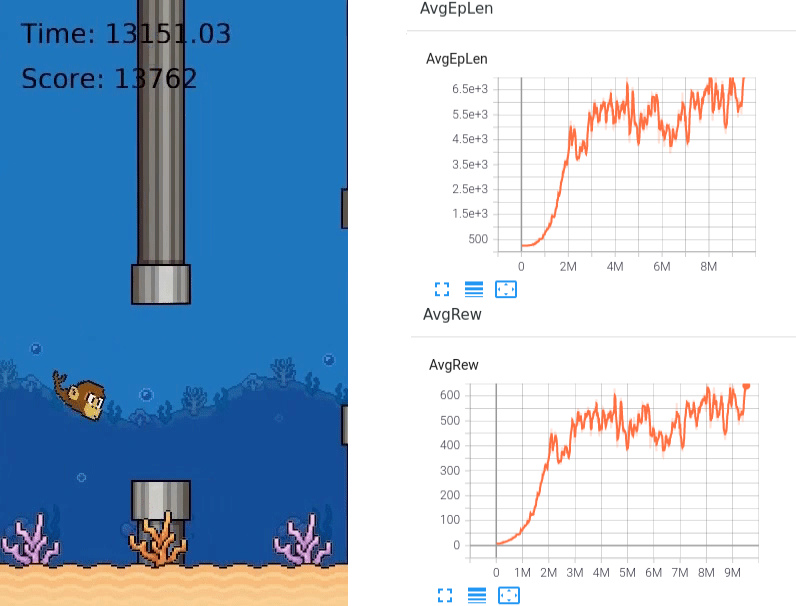
\includegraphics[scale=0.5]{img/I/Selection_101.png}
\centering
\captionsetup{justification=centering}
\caption{Demo, customized environment 2; (1) visual, (2) learning curves.}
\end{figure}

\pagebreak

\section{DQN Traffic Signal Control with Partial Detection}

In this second part, we present the work done during the second half of the internship, which consists of an application project of the DQN algorithm to traffic engineering. Here, we apply DQN to traffic light policy optimization based on limited detected information provided by connected vehicles, which represent a fraction of the total vehicle flow. The contribution is a DQN model for intelligent traffic signal control with partial detection.
The first section formalizes the problem and lays the background, with a review of terminology, literature of related work, and an industry-standard traffic simulation tool. The second section presents the proposed DQN model; DQN-ITSCwPD (DQN Intelligent Traffic Signal Control with Partial Detection), and exposes implementation details of the environment and comparison techniques. The third section presents the training and testing methods, and assesses the model by evaluating the performances over multiple scenarios. Efficiency thresholds are estimated by acceptable and optimal detection rates. \\
The project is available at: \textbf{\url{https://github.com/romainducrocq/DQN-ITSCwPD}}.

\subsection{Background}

In this first section of the second part, we introduce the problem and lay the background foundations, with a literature review of RL and DQN applications to intelligent traffic signal control and partially detected transportation systems. The problem and terminology are first formulated, followed by a review of the current related work and existing tools.

\subsubsection{Problem definition and terminology}

\textbf{Formulation of the problem} \\
We formulate the problem studied in this part and answered with this project as follows: 

\begin{table}[htbp]
\centering
\setlength\tabcolsep{2pt}
\begin{tabular}{|c|}
\hline
\\
\:\:A DQN agent controls the traffic light signals at an isolated intersection\:\:\\
\:\:with the aim to minimize the total travel time through the intersection,\:\:\\
\:\:in a partially observable environment with limited detected information\:\:\\
\:\:provided by a fraction of the total vehicle flow from connected vehicles.\:\:\\
\\
\hline
\end{tabular}
\end{table}

\textbf{Terminology} \\
We define here the transportation theory terminology used throughout this presentation. \\

(1) Network topology and movements:
\begin{itemize}
\setlength\itemsep{-0.5em}
  \item \textbf{Approach}: An approach is a roadway meeting at an intersection, and can be either incoming or outgoing. Vehicles enter the intersection through an incoming approach and leave the intersection through an outgoing approach. For intersections equipped with traffic signal devices, each incoming approach is controlled by a traffic light.
  \item \textbf{Lane}: An approach consists of a set of lanes, which are also either incoming lanes or outgoing lanes. Each incoming lane is controlled by one or many traffic signals.
  \item \textbf{Movement}: A movement refers to a vehicle crossing the intersection from an incoming approach to an outgoing approach, and it is right turn, left turn or through.
  \item \textbf{Connection}: A connection is a link between an incoming lane in an incoming approach and an outgoing lane in an outgoing approach. It enables for a vehicle to perform a movement across the intersection. An incoming lane has a set of connections to one or many outgoing lanes, each controlled by one own traffic signal.
\end{itemize}

(2) Traffic signals and traffic phases:
\begin{itemize}
\setlength\itemsep{-0.5em}
  \item \textbf{Traffic signal}: A traffic signal is a green, yellow or red indication that controls the movements at a connection. Connections are open at green signals, conditionally open at yellow signals and fully closed at red signals, with all movements prohibited.
  \item \textbf{State}: A state is the combination of traffic signals at the intersection, the traffic signals for all the connections of all the incoming lanes of all the incoming approaches.
  \item \textbf{Phase}: A phase is the complete sequence of the successive states and associated time intervals for opening a set of concurrent connections with non-conflicting movements. Phases are intended to separate conflicting connections, so that movements in a phase have no, or minimum, conflicts. A phase consists of a main green interval, either permissive or protected, followed by a change interval and a clearance interval.
  \item \textbf{Green interval}: A green interval, with duration $T_g$, is the first interval in a phase. It allows for some vehicles to cross the intersection along authorized movements from a set of non-conflicting open connections with green traffic signals, while the other connections are closed with red traffic signals. A green interval is either permissive, and conflicting left turns are authorized and made through gaps in oncoming traffic, or protected, and conflicting left turns are not authorized. The green interval is often set to be longer than a minimum green interval, to satisfy driver expectancy, queue clearance, and enable pedestrian crossing in parallel directions, i.e. $T_g \ge T_{g,min}$. 
  \item \textbf{Change interval}: A change interval, with duration $T_y$, follows the green interval as the second interval in a phase. It is a transition interval between two phases of non-conflicting authorized movements, with yellow traffic signals at the set of open connections from the previous green interval,  where vehicles can only cross if they can not stop safely before the stop line, and red traffic signals at other connections.
  \item \textbf{Clearance interval}: A clearance interval, with duration $T_r \ge 0$, is an optional last interval in the phase, and is used to clear the intersection before the green interval of the next phase. All traffic signals are red, and thus all connections are fully closed.
  \item \textbf{Phase interval}: The phase interval is the duration of the phase $T_p = T_g + T_y + T_r$.
  \item \textbf{Cycle}: A cycle is one complete rotation through all the phases at the intersection.
\end{itemize}

(3) Connected vehicles (CV):
\begin{itemize}
\setlength\itemsep{-0.5em}
  \item \textbf{Connected vehicles}: Connected vehicles (CV) are equipped with communication devices and can transmit information to traffic infrastructures, i.e. such as traffic signal controllers, which consists at least of the position and the speed of the vehicle.
  \item \textbf{CV penetration rate}: The connected vehicle penetration rate $p_{cv}$ is the proportion of connected vehicles in the total traffic flow. A mixed traffic comprises of a percentage $p_{cv}$ of connected vehicles and a percentage $1-p_{cv}$ of conventional vehicles.
  \item \textbf{Assumption on CV}: We make the assumption that connected vehicles are fully visible, i.e. their positions and speeds can be observed with perfect accuracy, and conventional vehicles are fully invisible. However, this assumption is debatable; e.g. [11] (Nguyen Van Phu, Farhi, 2020) reports that current GPS localization systems are not precise enough to know the lane in which a CV is situated, but only the approach. They thus provide a probabilistic approach to estimate the lengths of queues in 2-lanes incoming approaches in a mixed traffic scenario. Here, we assume that positions and speeds of CVs are perfectly observable, either through the use of improved technologies or by similar estimation methods applied upstream to data.
\end{itemize}

\subsubsection{Literature review of related work}

\textbf{RL in traffic control} \\
Traffic engineering raises numerous optimal control problems, and as such has been widely studied from the perspective of reinforcement learning. With the main actors of traffic being vehicles, and with the emergence of mixed-autonomy traffic in a near future due to the arrival of automated vehicles, which evolve in road network environments with continuous action spaces, a large portion of the recent studies are addressed by actor-critics and policy-based deep RL algorithms; such as A3C, DDPG, TRPO and PPO.
E.g.; car following on closed networks and shock wave dissipation, lane changing and insertion models, bottleneck decongestion, highway on-ramp merging, and emergent behaviors in mixed-autonomy traffic [12,13,14,15]. Moreover, other traffic actors, such as infrastructures among which traffic lights, present control problems to be optimized in discrete action spaces. This has led researchers to apply DQN algorithms to traffic signal control. \\

\textbf{DQN for traffic signal control} \\
Traffic congestion poses serious economical and social problems; long travelling times, fuel consumption and air pollution; and inefficient traffic signals are significant underlying root causes to the issue. Fixed time traffic signals with predetermined timing have been commonly used, but become inadequate when facing dynamic and varying traffic demands. Thus, with ever growing urban areas and vehicle fleets, adaptive traffic signal control, able to respond to traffic flows in real time, is sought as a major stake of urbanization.
Traffic signal control (TSC) has been addressed by RL methods even before the deep learning era, with Markov chains, dynamic programming, fuzzy logic and discrete tabular Q-learning [16]. However, the advent of deep Q-learning in recent years has enabled to explore many novel TSC applications based on DQN algorithms. Initial studies with simpler models have proven DQN to be efficient for traffic signal control, comparing trained MLP models at isolated intersection with other algorithms from the literature [17,18]. Following studies have build on these models to explore the benefits of complex neural networks architectures, with stacked auto encoders, convolutional neural networks and recurrent neural networks [19,20,21,22,23,24]. Latest work also successfully demonstrated a complete state-of-the-art rainbow DQN implementation for TSC, with adaptations of the six DQN extensions [25]. Furthermore, a significant portion of the research in the field is dedicated to achieve decentralized coordination between traffic lights, with applications of multi agent reinforcement learning (MARL) over up to 1000 coordinated agents [26,27,28,29]. Yet, the main focus and effort in the literature is put on defining state representations and reward functions. Indeed, the complexity of traffic environments, composed of many individual actors interacting together with unpredictable behaviors, leaves these as unresolved questions, with numerous propositions and no overall consensus. \\

\textbf{TSC with connected vehicles} \\
TSC responds to traffic demand based on real time measures of road traffic parameters. While the data are easily recovered in software simulations, real world implementations rely on expensive infrastructures, which exists only at a small fraction of intersections. These are mainly inductive loops under the roads, which allow for macroscopic representations of the traffic, or, in rare cases, radars or video cameras for microscopic descriptions. Most TSC propositions mentioned above require information that are thus difficult to obtain, and are for now mostly inapplicable. However, the rapid  development of IoT has created new technologies applicable for sensing vehicles, such as GPS localization systems, dedicated short ranged communications (DSRC), C-V2X, radio frequency identification, Bluetooth, ultra wide band, Zigbee, and apps (e.g. Google Maps) [11,30]. These communication devices are cost-effective, and do not require heavy infrastructure set ups. An increasing number of equipped connected vehicles are thus nowadays able to transmit their positions and speeds to nearby equipment, allowing for microscopic partial state representations of intersections. Furthermore, latest research have shown that TSC with partial detection applied to CV penetration rates as low as 20\% can significantly improve traffic conditions for all vehicles [31]. These however only consider agents trained over fixed CV penetration rates, which is an unrealistic scenario. DQN applications for TSC with partial detection over connected vehicles have been very little investigated for the time being, and are listed by recent surveys as a gap in the literature and a key future research. \\

\textbf{TSC actions, observations and rewards} \\
The main effort in the literature of TSC with DQN has been placed on the definition of efficient state representations and reward functions. However, RL models are time consuming to tune, and the complexity of TSC environments makes evaluation difficult. Moreover, the issue of reproducibility in RL prevents rigorous comparison of TSC models. Thus, there are for now no widely accepted representations, and many have been proposed. We compile here a non-comprehensive list of agent specifications found in the literature:
\begin{itemize}
\setlength\itemsep{-0.5em}
  \item \textbf{Actions}: Two main types of actions exists; either (1) the TSC agent acyclically selects the next phase from a set of possible phases with fixed green interval duration [17,19,21,24,25,26,27,28,29,30,31,32,33], or (2) the TSC agent selects the duration of the next green interval for the upcoming phase in a predetermined cycle [18,22,23].
  \item \textbf{Observations}: The state representations can either be macroscopic, with estimations of global parameters over traffic flows, or microscopic, with raw data for individual vehicles. While earlier work based on discrete tabular Q-learning or shallow DQN preferred low-dimensional macroscopic state representations, latest work observe individual vehicles for high-dimensional microscopic state representations. Indeed, a significant gain in performance has been measured for microscopic observations over macroscopic ones [32]. Either way, state representations have been usually found to be aggregations of multiple traffic features; among which current phase [18,21,23,26,27,28,29,30,31], number of vehicles [18,23,25,28,30,31,32], positions of vehicles [21,22,23,24,26,32], queue lengths [18,19,23,32,33], speeds of vehicles [17,21,22,32], history of past phases [17,25,32], elapsed time in the current phase [30,31], green, change and clearance intervals duration [30,31], distances to nearest vehicles [30,31], pressures [27,29], number of waiting vehicles [17], waiting times of vehicles [23], and upcoming phase in a cycle [23]; i.e over approaches, lanes or other.
  \item \textbf{Rewards}: The reward functions in TSC, overall, aim at reducing vehicular time loss caused by traffic signals. As such criterion can not be assessed directly, rewards are mostly defined as weighted combinations of traffic features, which coefficients are set empirically. The lack of solid theoretical justifications is a major challenge for real world deployment, as RL rewards are difficult to transcribe mathematically without distorting the intended goal, especially in complex systems. Here, the reward functions act in effect as punishments, and with agents reducing evaluation metrics derived from traffic features, i.e. maximizing negative values; among which delays of vehicles [18,23,26,30,31,32,33], waiting times of vehicles [21,22,23,25,26], queue lengths [19,23,28,33], intersection throughput [17,23,25,33], phase changes [23,25,26], pressures [27,29], accumulated waiting times of vehicles [24], number of waiting vehicles [25], travel times of vehicles [23], emergency stops  of vehicles [26], and teleports of vehicles (in Sumo) [26]; i.e. over approaches, lanes or other, and over cumulative values, averages, relative differences, individual vehicles, or other. 
\end{itemize}

\pagebreak

\newgeometry{left= 3cm, right= 2cm, bottom= 0cm, top= 2.6cm}

\subsubsection{Traffic simulation with Sumo}

\textbf{Traffic simulators as RL environments} \\
Traffic networks are complex stochastic environments, where many actors concurrently evolve in a shared space, i.e. vehicles, pedestrians, infrastructures. At the particle scale, the uncoordinated interactions between drivers with conflicting interests, each minimizes its travel time, create unpredictable behaviors. At the global scale, they are bound by the laws of traffic flow physics and dynamics, with perturbations propagated and amplified. Hence, TSC relies on the use of industry-standard software traffic simulators, based on microscopic mathematical models and differential calculus over longitudinal and lateral vehicle dynamics [12]. These allow to develop RL control strategies with high-fidelity state representations, and test them over large and heterogeneous road networks and scenarios. The main traffic simulators used in the TSC research community are Sumo, Aimsum, Cityflow, Paramics and Matsim [34]. As part of this project, we use the Sumo simulator. \\

\textbf{SUMO, Simulation of Urban MObility} \\
Sumo (simulation of urban mbility) [35], is an open source, microscopic, continuous and industry-standard traffic simulation software and package of tools for modeling large road networks with high fidelity, developed by the German Aerospace Center (DLR) since 2001. \\ 
It allows for complex scenario generation with decentralized and multi modal simulated objects, including vehicles, pedestrians and infrastructures. Traffic scenarios are designed in a set of \texttt{XML} configuration files, where simulation data are specified, i.e. they define (1) network structures with intersections, approaches, lanes and connections, (2) traffic demands with vehicle insertion times and routes, and (3) traffic lights with signal programs; and can be created in the visual network editor \texttt{netedit}. Networks can be both synthetic, or converted from real world OSM data. Furthermore, Sumo comes with two python code interfaces to embed the simulated environment within larger programs, the \texttt{sumolib} and \texttt{traci} libraries. These contain modules and functions for interacting online with simulations in real time, and provide control over the simulated networks and agents. Sumo can be used either from the command line interface with simulations over sub processes, or with a graphical user interface, with the \texttt{sumo} and \texttt{sumo-gui} packages.

\begin{figure}[h]
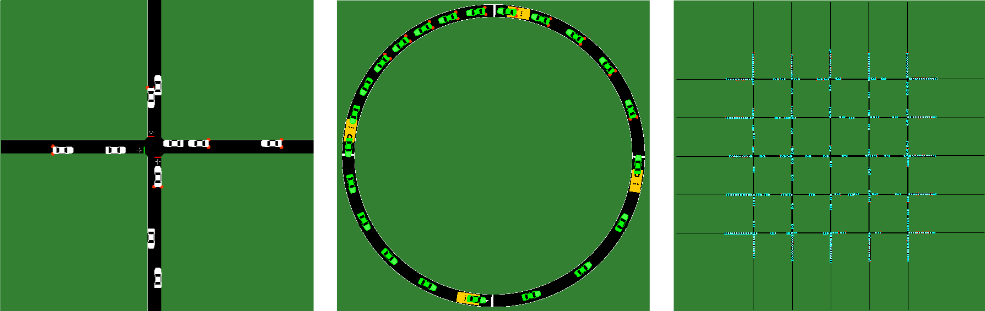
\includegraphics[width=\textwidth]{img/II/Selection_111.png}
\centering
\captionsetup{justification=centering}
\caption{Sumo GUI visuals.}
\end{figure}

\restoregeometry

\pagebreak
\subsection{Method}

In this second section of the second part, we describe the developed solution to the problem introduced hereinabove, with an overview of the software implementation of the project.
We mainly present the proposed DQN model; DQN-ITSCwPD (DQN Intelligent Traffic Signal Control with Partial Detection). We also detail the customized environment implemented with the Sumo traffic simulator, and two  algorithms as comparison baselines. 

\subsubsection{Environment implementation}

\textbf{Customized environment in frameworQ} \\
As mentioned before, the application project is implemented within frameworQ, the DQN framework for customized environments (see part 1.3). Hence, only the customized environment is added in the \texttt{env/} package, with the rest of the architecture left unchanged. The environment model encompasses a Traci interface for traffic signal control in the Sumo traffic simulator, and the corresponding Sumo configuration files, as well as the DQN controller and additional resources. An installation script is provided to build the project and its dependencies, with the \texttt{sumo} software as a local \texttt{venv/} package, at \texttt{bin/make.sh}. \\

\textbf{Sumo simulation configuration data} \\
In the Sumo traffic simulator, simulation scenarios are defined by \texttt{XML} configuration data files. In the project environment, a \texttt{data/} folder contains these \texttt{XML} configuration data files, with one sub-folder per simulation scenario. A \texttt{.net.xml} file, created with the \texttt{netedit} visual network editor, configures the network, with the approaches, lanes and connections for all the roads and intersections. A \texttt{.tll.xml} file configures the traffic signal logic, with the programs of the traffic lights in the network. The programs contain all the possible phases, which are represented as the sequences of signals over a complete clockwise rotation around an intersection. A \texttt{.rou.xml} file configures the route definitions, i.e. the possible itineraries in the network, and the traffic demand over these itineraries. It first lists the routes as the sequences of their consecutive approaches, then the types of vehicles that can be inserted in the network, and finally the traffic demand for the simulation as all the individual vehicles to be inserted, by time of insertion in the network and with their respective itineraries. Contrary to the two previous configuration files that are fixed, the route configuration file is intended to change between simulations as the traffic demand vary. A \texttt{.sumocfg} file serves as an entry point to the simulator for a given simulation scenario, by grouping the paths to the aforementioned configuration files. Finally, an optional \texttt{gui-settings.cfg} file configures the visual settings for the graphical interface \texttt{sumo-gui}. \\

\textbf{Sumolib-Traci interface for Sumo TSC} \\
Sumo provides two python tools for interfacing the traffic simulator. The \texttt{sumolib} library provides a set of static methods to parse configuration files and retrieve network structural information. The \texttt{traci} library provides a set of methods to interact dynamically with the simulated objects in real time, both to retrieve and to modify data online. Both tools are used in the \texttt{sumo\_env.py} file, a Sumo traffic signal control interface. As the DQN model is intended to be run on a wider range of traffic situations, the interface is designed to be flexible towards parameterized traffic scenario loading and traffic demand generation, and thus contains no hard coded information. The simulations are handled by a two-step process, with an initial mapping procedure and episodic traffic demand generation. At each episode, a simulation is started and run on a \texttt{traci} sub-process from the configuration files in the corresponding \texttt{data/} sub-folder, with either \texttt{sumo} or \texttt{sumo-gui}. \\ 

\textbf{Initialization mapping procedure} \\
In the \texttt{sumolib-traci} TSC interface, an initial mapping procedure enables to dynamically load new traffic scenarios from a \texttt{data/} sub-folder without hard coded information, prior to starting the first simulation. Firstly, the road network is parsed with \texttt{sumolib} to create two structural maps. The map of intersections with traffic lights is recovered, along with their respective maps of incoming and outgoing approaches and lanes. The map of possible routes is generated by applying the Dijkstra path finding algorithm between all combinations of entry and exit approaches in the network. Secondly, an empty simulation, that is with no traffic demand and killed instantly, is launched with \texttt{traci} to create the map of traffic signal logic. This, by completing a full cycle of phases for every traffic light programs, along with their respective maps of green interval signals and open connections. \\

\textbf{Episode traffic demand generation} \\
In the \texttt{sumolib-traci} TSC interface, new traffic demand is generated at each simulation, i.e. each episode, to create unseen traffic situations for the DQN agent. At each episode, each entry approach $e$ in the network is assigned an insertion traffic flow $q_e$, in vehicles per hour. From these traffic flows, traffic demand is generated for each entry approach by a Poisson process with rate $\lambda_e = q_e^{-1}\cdot 3600$ over the duration of the simulation. For each entry approach, the vehicles are randomly distributed over the connections of the intersection, such that the insertion traffic flow is proportionally split over the possible routes. Each episode is also assigned a CV penetration rate $p_{cv}$, and a proportion of $p_{cv}$ vehicles are identified as connected, while the complementary proportion of $1-p_{cv}$ vehicles are identified as conventional. The total traffic demand is sorted by insertion time in the simulation, and written to the \texttt{.rou.xml} route configuration file, with the corresponding routes listed in the initialization mapping procedure and special vehicle types for CV and non-CV. The insertion traffic flows $q_e$ and the CV penetration rate $p_{cv}$ can either be set manually as hyper-parameters, or be chosen randomly at each episode of simulation. \\

\textbf{Scheduler for multiple TL control} \\
The timesteps experienced by the DQN agent as part of the decision making problem do not coincide with the internal clock refresh rate in the simulation, that is every second. Moreover, a delay is introduced between the decision to change phase and the actual phase change, as the phase transition between two green intervals goes through intermediate change and clearance intervals. Finally, in a traffic scenario with multiple intersections, this delay can induce overlaps between the time intervals over the different traffic lights. \\
We introduce a special data structure for scheduling phase changes in \texttt{
tl\_scheduler.py}, to counter these problems. This traffic light scheduler stores the upcoming phase changes planned for each traffic light, and effectively performs these transitions with respect to the green, change and clearance intervals. The adequate number of internal transitions are completed in the simulator and abstracted from the DQN agent, which is called only upon decision making. Thus, this scheduling data structure enables to control multiple traffic lights without time interference, despite centralized transition dynamics in Sumo.

\subsubsection{DQN-ITSCwPD model}

\textbf{DQN control with Per3DQN+} \\
As mentioned before and as part of frameworQ, traffic signal control is conducted with the Per3DQN+ algorithm (see part 1.3.2). We present here the proposed DQN model; DQN-ITSCwPD (DQN Intelligent Traffic Signal Control with Partial Detection), i.e. the action, observation and reward functions, the neural network and the hyper-parameters. The three former are implemented in \texttt{rl\_controller.py}, inherited from \texttt{sumo\_env.py} with \texttt{traci} and encapsulated in \texttt{dqn\_env.py}, and the two latter are defined in \texttt{dqn\_config.py}.\\

\textbf{Action: phase selection} \\
The agent selects the next phase for the next $T_g$ seconds of green time interval among the set of all possible phases, at a given traffic light. If the selected phase is the same as the current phase, the current green interval is extended by $T_g$ seconds. Else, a transition to the next phase is executed, with an intermediate $T_y + T_r$ seconds through change and clearance intervals, and an initial $T_g$ seconds in the green interval of the selected phase. Thus, while the action is formally to select the next phase, the agent also indirectly decides the duration of the current phase by selecting the same phase multiple times consecutively. \\

\textbf{Action space: size 2 or 4} \\ 
The action space is defined by the number of possible phases in the traffic light program. At a four-way intersection, there is a total of 8 valid paired signal phases for non-conflicting movement signals [34]. From this, the set of possible phases, i.e. with no or minimum conflicts, has either 2, 4 or 8 phases, and are as follows with their respective action spaces:
\begin{itemize}
\setlength\itemsep{-0.5em}
  \item \textbf{2 phases}: 2-phases programs are used for small intersections and traffic flows, with conflicting left turns authorized. They have two permissive green intervals, one for each axis, with permissive turn left, through and turn right movements. The first phase, along the north-south axis, is (1) from north to east, south and west, and from south to west, north and east. The second phase, along the east-west axis, is (2) from east to south, west and north, and from west to north, east and south. The action space is $A=\{(n\rightarrow esw,s\rightarrow wne),(e\rightarrow swn,w\rightarrow nes)\}$, with size $|A|=2$.
  \begin{figure}[h]
    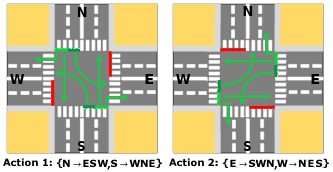
\includegraphics[scale=0.8]{img/II/2phases.png}
    \centering
    \captionsetup{justification=centering}
    \caption{2 phases, action space.}
  \end{figure}
  \item \textbf{4 phases}: 4-phases programs are used over medium to large intersections and traffic flows, with protected left turns only. They have four protected green intervals, two for each axis, with protected turn left movements only, or through and turn right movements. The first and second phases, along the north-south axis, are (1) from north to south and west, and from south to north and east, and (2) from north to east, and from south to west. The third and fourth phases, along the east-west axis, are (3) from east to west and north, and from west to east and south, and (4) from east to south, and from west to north. The action space is $A=\{(n\rightarrow sw,$ $s\rightarrow ne),(n\rightarrow e,s\rightarrow w),(e\rightarrow wn,w\rightarrow es),(e\rightarrow s,w\rightarrow n)\}$, with size $|A|=4$.
  \begin{figure}[h]
    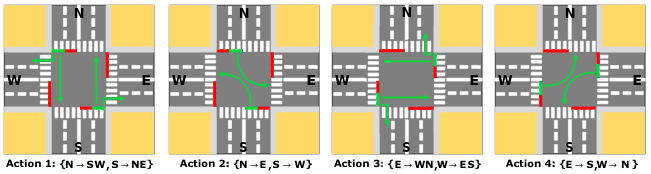
\includegraphics[scale=0.8]{img/II/4phases.png}
    \centering
    \captionsetup{justification=centering}
    \caption{4 phases, action space.}
  \end{figure}
  \item \textbf{8 phases}: 8-phases programs are used rarely in practice, and are not studied here.
\end{itemize}

\textbf{Observation: partial DTSE} \\
Discrete traffic state encoding (DTSE) [20] (Gao et al., 2017) is a microscopic, image-like state representation of the intersection for TSC. Here, we adapt DTSE to the partially observed environment with detection on connected vehicles, and propose partial DTSE.

\pagebreak

\newgeometry{left= 3cm, right= 2cm, bottom= 0cm, top= 2.6cm}

In partial DTSE, the state representation is an image-like construction of stacked 2D-matrices for multiple levels of microscopic, individual information provided by connected vehicles and traffic signals at the intersection. Here, all incoming lanes are discretized, over segments from the stop line up to a detection range less than or equal to the total length of the corresponding approach, into grids with cells of fixed length, set to be slightly larger than the average size of a vehicle with inter-vehicle gap. The cells contain data on individual CVs and traffic signals, and the grids are aggregated over the segments. Three 2D-matrices are extracted for three levels of information; i.e. the matrix of CV positions $P$, the matrix of CV speeds $V$, and the matrix of traffic signals over lanes $S$; and stacked into a single image-like state representation of the intersection; partial DTSE: \\
\[ \text{Partial DTSE} = \{P = [P_0, P_1, P_2, P_3]; V = [V_0, V_1, V_2, V_3]; S = [S_0, S_1, S_2, S_3] \} \]

\begin{figure}[h]
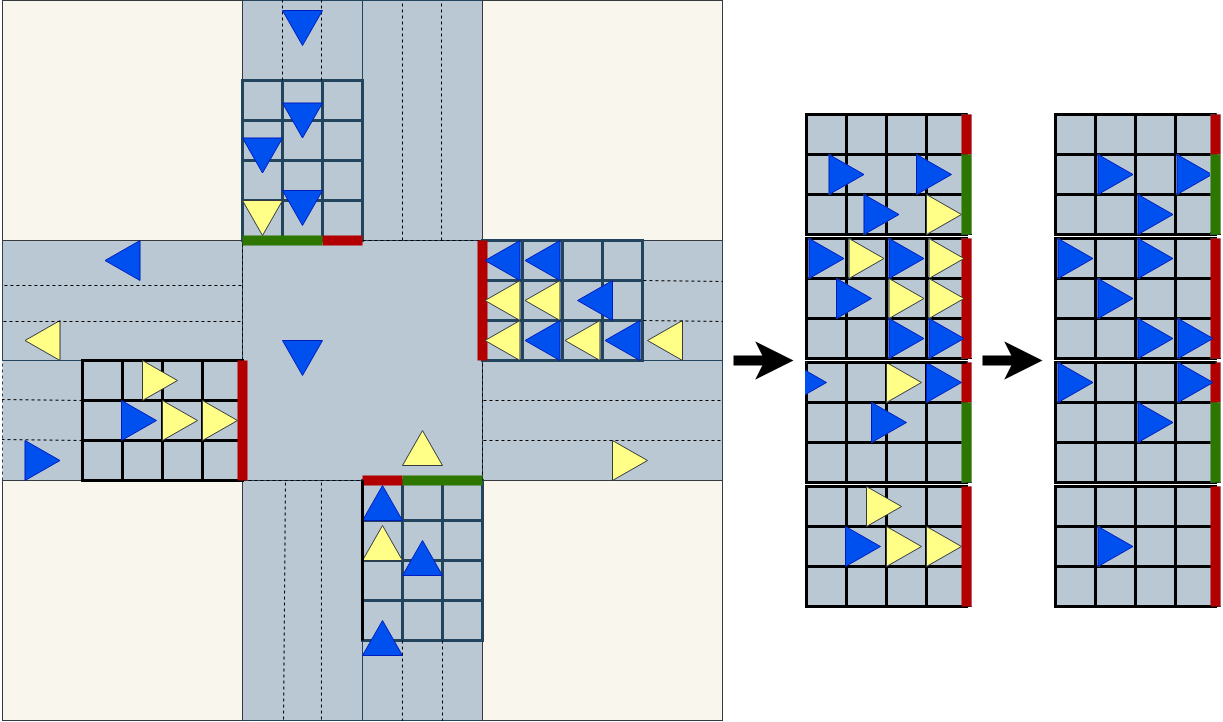
\includegraphics[width=\textwidth]{img/II/pdtse_full.png}
\centering
\end{figure}

\begin{table}[!htbp]
\centering
\setlength\tabcolsep{2pt}
\begin{tabular}{c}
Partial DTSE = 
\end{tabular}
\begin{tabular}{|c|c|c|c|}
\hline
\multicolumn{4}{|c|}{$P = [P_0, P_1, P_2, P_3]$} \\
\hline
\:\: 0 \:\: & \:\: 0 \:\: & \:\: 0 \:\: & \:\: 0 \:\: \\ \hline
\:\: 0 \:\: & \:\: 1 \:\: & \:\: 0 \:\: & \:\: 1 \:\: \\ \hline
\:\: 0 \:\: & \:\: 0 \:\: & \:\: 1 \:\: & \:\: 0 \:\: \\ \hline
\:\: 1 \:\: & \:\: 0 \:\: & \:\: 1 \:\: & \:\: 0 \:\: \\ \hline
\:\: 0 \:\: & \:\: 1 \:\: & \:\: 0 \:\: & \:\: 0 \:\: \\ \hline
\:\: 0 \:\: & \:\: 0 \:\: & \:\: 1 \:\: & \:\: 1 \:\: \\ \hline
\:\: 1 \:\: & \:\: 0 \:\: & \:\: 0 \:\: & \:\: 1 \:\: \\ \hline
\:\: 0 \:\: & \:\: 0 \:\: & \:\: 1 \:\: & \:\: 0 \:\: \\ \hline
\:\: 0 \:\: & \:\: 0 \:\: & \:\: 0 \:\: & \:\: 0 \:\: \\ \hline
\:\: 0 \:\: & \:\: 0 \:\: & \:\: 0 \:\: & \:\: 0 \:\: \\ \hline
\:\: 0 \:\: & \:\: 1 \:\: & \:\: 0 \:\: & \:\: 0 \:\: \\ \hline
\:\: 0 \:\: & \:\: 0 \:\: & \:\: 0 \:\: & \:\: 0 \:\: \\ \hline
\end{tabular}
\begin{tabular}{|c|c|c|c|}
\hline
\multicolumn{4}{|c|}{$V = [V_0, V_1, V_2, V_3]$} \\
\hline
\:\: 0 \:\: & \:\: 0 \:\: & \:\: 0 \:\: & \:\: 0 \:\: \\ \hline
\:\: 0 \:\: & 0.9 & \:\: 0 \:\: & 0.8 \\ \hline
\:\: 0 \:\: & \:\: 0 \:\: & 0.8 & \:\: 0 \:\: \\ \hline
\:\: 0 \:\: & \:\: 0 \:\: & \:\: 0 \:\: & \:\: 0 \:\: \\ \hline
\:\: 0 \:\: & 0.2 & \:\: 0 \:\: & \:\: 0 \:\: \\ \hline
\:\: 0 \:\: & \:\: 0 \:\: & \:\: 0 \:\: & \:\: 0 \:\: \\ \hline
0.4 & \:\: 0 \:\: & \:\: 0 \:\: & \:\: 0 \:\: \\ \hline
\:\: 0 \:\: & \:\: 0 \:\: & 0.7 & \:\: 0 \:\: \\ \hline
\:\: 0 \:\: & \:\: 0 \:\: & \:\: 0 \:\: & \:\: 0 \:\: \\ \hline
\:\: 0 \:\: & \:\: 0 \:\: & \:\: 0 \:\: & \:\: 0 \:\: \\ \hline
\:\: 0 \:\: & 0.1 & \:\: 0 \:\: & \:\: 0 \:\: \\ \hline
\:\: 0 \:\: & \:\: 0 \:\: & \:\: 0 \:\: & \:\: 0 \:\: \\ \hline
\end{tabular}
\begin{tabular}{|c|c|c|c|}
\hline
\multicolumn{4}{|c|}{$S = [S_0, S_1, S_2, S_3]$} \\
\hline
\:\: 0 \:\: & \:\: 0 \:\: & \:\: 0 \:\: & \:\: 0 \:\: \\ \hline
\:\: 1 \:\: & \:\: 1 \:\: & \:\: 1 \:\: & \:\: 1 \:\: \\ \hline
\:\: 1 \:\: & \:\: 1 \:\: & \:\: 1 \:\: & \:\: 1 \:\: \\ \hline
\:\: 0 \:\: & \:\: 0 \:\: & \:\: 0 \:\: & \:\: 0 \:\: \\ \hline
\:\: 0 \:\: & \:\: 0 \:\: & \:\: 0 \:\: & \:\: 0 \:\: \\ \hline
\:\: 0 \:\: & \:\: 0 \:\: & \:\: 0 \:\: & \:\: 0 \:\: \\ \hline
\:\: 0 \:\: & \:\: 0 \:\: & \:\: 0 \:\: & \:\: 0 \:\: \\ \hline
\:\: 1 \:\: & \:\: 1 \:\: & \:\: 1 \:\: & \:\: 1 \:\: \\ \hline
\:\: 1 \:\: & \:\: 1 \:\: & \:\: 1 \:\: & \:\: 1 \:\: \\ \hline
\:\: 0 \:\: & \:\: 0 \:\: & \:\: 0 \:\: & \:\: 0 \:\: \\ \hline
\:\: 0 \:\: & \:\: 0 \:\: & \:\: 0 \:\: & \:\: 0 \:\: \\ \hline
\:\: 0 \:\: & \:\: 0 \:\: & \:\: 0 \:\: & \:\: 0 \:\: \\ \hline
\end{tabular}
    \captionsetup{justification=centering}
    \captionof{figure}{Partial DTSE.}
\end{table}

\restoregeometry

\pagebreak

The above example demonstrates partial DTSE applied to a four-way intersection, with connected vehicles in blue and conventional vehicles in yellow. The matrix of CV positions $P$ is binary encoded, with 1 and 0 being respectively the presence or absence of connected vehicles in the cells. The matrix of CV speeds $V$ encodes the corresponding speeds, normalized over the speed limits of approaches. The matrix of traffic signals over lanes $S$ is binary encoded, with 1 being a green signal for the lane and 0 another signal.
In Sumo, the vehicle size and inter-vehicle gap are 5 and 2.5 meters. Thus, we use cells of 8 meters, and a detection range of 160 meters, i.e. sensing up to twenty CVs per lane. \\

\textbf{Reward: total squared delay} \\
The goal of the agent is to minimize the total travel time through the intersection for all commuters, i.e. for both connected and conventional vehicles. As such, while the state represents only CVs in a partially observed environment, the reward function considers all vehicles in a fully observed environment. This implies that full training is completed in the simulator, where conventional vehicles are observable, and performances do not improve after deployment [30]. We propose a reward function based on vehicle delay, as delay was considered the most efficient metric for learning by a comparative study [33]. Minimizing delay translates to minimizing the lost travel time $\overline{t} - t_{min}$, with $\overline{t}$ the average travel time of vehicles and $t_{min}$ the lowest possible travel time with speed limit $v_{max}$ [30]. Over the travel distance $t_{min} \cdot v_{max}$, for a given vehicle $i$ with speed $v_i(t)$, and at time $t$:

\[ t_{min} \cdot v_{max} = \int_{0}^{\overline{t}} v_i(t) \,dt \implies t_{min} = \frac{1}{v_{max}} \int_{0}^{\overline{t}} v_i(t) \,dt \]

\[ \implies \overline{t} - t_{min} =  \int_{0}^{\overline{t}} 1 \,dt - \frac{1}{v_{max}} \int_{0}^{\overline{t}} v_i(t) \,dt = \frac{1}{v_{max}} \int_{0}^{\overline{t}} v_{max} - v_i(t) \,dt \]
\\
Thus, minimizing the delay is equivalent to minimizing, for each timestep $t$ and vehicle $i$:

\[ d_i(t) = \frac{1}{v_{max}} \cdot ({v_{max}} - v_i(t)) = 1 - \frac{v_i(t)}{v_{max}} \]
\\
The goal is to decrease the delay for all vehicles, and we hence use a cumulative metric. Total delay is preferred over average delay, as it retains information on the volume of vehicles at the intersection. Moreover, we apply a power term so that fewer large delays are prioritized over many short delays, which encourages fairness between vehicles. Besides, exponents in reward functions are empirically known to boost learning, as they emphasize small performance gains towards the objective. Thus, we present the total squared delay:
\[ tsd(t) = \sum_{i} (1 - (\frac{v_i(t)}{v_{max}})^2) \]

\pagebreak

\newgeometry{left= 3cm, right= 2cm, bottom= 0cm, top= 2.6cm}

As rewards are maximized, minimizing a metric equates to maximizing its negated value. Here, the reward function acts in effect as a punishment, by maximizing the negative total squared delay. Additionally, the reward is normalized by the maximum total squared delay encountered at that time of training $tsd_{max}(t) = \max (tsd(t), tsd_{max}(t-1))$, and centered in $[0, 1]$ for learning stability [18]. Thus, the complete TSC reward function is given by:
\[ r(t) = 1 - \frac{tsd(t)}{tsd_{max}(t)} = 1 - \frac{\sum_{i} (1 - (\frac{v_i(t)}{v_{max}})^2)}{\max (tsd(t), tsd_{max}(t-1))}\]
\\
\textbf{Convolutional NN, hyper-parameters} \\
The convolutional neural network (CNN) [36] (Krizhevsky et al., 2012) is a special NN architecture for image analysis. The underlying principles of forward and back propagation apply as presented earlier, but the architecture is split into two distinct learning modules. \\
A first learning module, the convolutional module, is composed of convolutional layers, that assemble patterns of increasing complexity in data with space invariant operations. They perform 2D-convolutions over shared weights of filters, or kernels, sliding with a stride along stacked input feature 2D-matrices called channels, to output feature maps. Additionally, optional intermediate pooling layers reduce the dimensions of the feature maps. Thus, a convolutional layer is defined by a number of channels $C$, a kernel size $K$ and a stride $S$. The output from the last convolutional layer is flattened and passed to a second learning module, the fully connected module, a MLP with fully connected layers. \\
Here, partial DTSE is a 3-channels image-like state representation with cells acting as pixels, and thus a convolutional dueling DQN maps from partial DSTE observations to phase selection actions. After experiments, we shaped the CNN to have two convolutional layers and two fully connected layers; i.e. $CNN1$ with $(C=16,K=4,S=2)$, $CNN2$ with $(C=32,K=2,S=1)$, $FC1$ with $128$ neurons and $FC2$ with $64$ neurons. Adding the input, dueling and aggregation output layers, the convolutional dueling DQN is as follows: \\

\begin{figure}[h]
  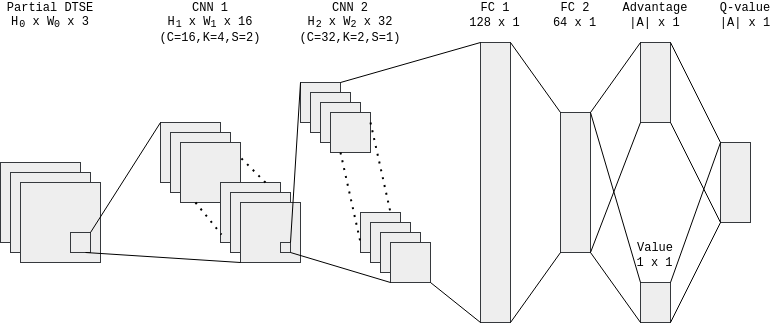
\includegraphics[width=\textwidth]{img/II/cnn_dueling.png}
  \centering
  \captionsetup{justification=centering}
  \caption{Convolutional dueling DQN.}
\end{figure}

\restoregeometry

\pagebreak

The model was tuned by grid search over the hyper-parameters, with tuning runs set to $200000$ timesteps. The tuned hyper-parameters are $\alpha=\num{1e-4}$ with Adam optimizer and Huber loss, $\gamma=0.99$, $\epsilon_{min}=0.01$, $\epsilon_{dec}=2$M with exponential decay, $N=1$M, $N_{min}=0.1$M, $\tau=\num{1e-3}$ with soft Polyak update. No terminal state is defined for the agent, and episodes are early stopped by an internal time limit in the Sumo simulation.

\subsubsection{Comparison baselines}

\textbf{Actuated TSC baselines}\\
Actuated traffic signal controllers are adaptive, non-learning TSC algorithms, responding to traffic flows in real time by measuring requests for green signals over the competing phases, according to fixed rules [34]. They rely on full, macroscopic traffic detection and are already extensively deployed at real intersections with inductive loops under the roads. 
As there exist, for the time being, no standard algorithm for deep Q-learning TSC with partial detection, neither deployed nor in the literature, we compare the proposed model to two actuated TSC algorithms; i.e. Max Pressure and SOTL [18]. These comparison baselines are implemented in \texttt{baselines.py}, inherited from \texttt{sumo\_env.py} with \texttt{traci}. \\

\textbf{Max Pressure}\\
Max Pressure (Varaiya, 2013) [37] is an acyclic actuated TSC algorithm which minimizes the pressure of phases at an intersection. The pressure of a phase $p$ at an intersection is defined as the difference between the total number of vehicles in the set of all incoming lanes with authorized movements for that phase $L_{p,inc}$ and the total number of vehicles in the set of all corresponding outgoing lanes $L_{p,out}$; i.e. $pressure(p) = \sum_{l \in L_{p,inc}} |V_l| - \sum_{l \in L_{p,out}} |V_l|$. \\
After each green interval of time $T_g$, the controller selects the phase $p \in P$ with maximum pressure to be relieved in the set of all possible phases. If the selected phase is the same as the current phase, the current green interval is extended by $T_g$ seconds. Else, a transition to the next phase is executed, with an intermediate $T_y + T_r$ seconds through change and clearance intervals, and an initial $T_g$ seconds in the green interval of the selected phase. While Max Pressure is an efficient and simple to implement actuated TSC algorithm, it presents a major drawback as it involves detection on vehicles in both incoming and outgoing lanes, and thus requires twice as much infrastructure and cost at real intersections. \\

\textbf{SOTL}\\
Self-organizing traffic lights (SOTL) (Gershenson, 2004) [38] is a cyclic actuated TSC algorithm which dynamically sets the green interval duration $T_g$ in the current phase $p$. \\
(1) A time integral $\kappa$ of the total number of vehicles in the set of all incoming lanes with prohibited movements for that phase $L_{inc} - L_{p,inc}$ and in a distance $\psi$ from the stop line is accumulated, and the current phase is maintained until the accumulated time integral reaches a fixed threshold $\theta$; i.e. $T_g$ = $T_g+1$, while $\kappa \le \theta$, with $\kappa = \kappa + \sum_{l \in L_{inc} - L_{p,inc}} |V_{l,\psi}|$.
(2) In addition to (1), small vehicle platoons of size $n$, the total number of vehicles in the set of all incoming lanes with authorized movements for that phase $L_{p,inc}$ and in a distance $\omega \le \psi$ from the stop line, are kept together and prevent phase changes for sizes less than a fixed threshold $\mu$; i.e. $T_g$ = $T_g+1$, if $0 < n \le \mu$, with $n = \sum_{l \in L_{p,inc}} |V_{l,\omega}|$.
According to (1) and (2), else, a transition to the next phase is executed, with an intermediate $T_y + T_r$ seconds through change and clearance intervals, and an initial $T_g$ seconds in the green interval of the next phase $p \in P$ in the cycle. Here, the constants are set to values commonly found in the literature; i.e. $\theta = 50$, $\mu = 3$, and $\psi = 80$, $\omega = 25$ meters. \\

\textbf{Algorithms}\\
The pseudo codes presented hereinafter are highly summarized, and do not include the phase transition procedure, nor the TL scheduling and the integration of Sumo dynamics. \\

\begin{algorithm}[H]
\small
\caption*{Max Pressure algorithm}
\begin{algorithmic}
    \IF{$T_g \ge T_{g,min}$}
        \STATE Set the next phase to maximum pressure phase $p = arg\max(\{pressure(p) \textbf{ for } p \in P\})$
        \STATE with $pressure(p) = \sum_{l \in L_{p,inc}} |V_l| - \sum_{l \in L_{p,out}} |V_l|$;
    \ENDIF
\end{algorithmic}
\end{algorithm}

\begin{algorithm}[H]
\small
\caption*{SOTL algorithm}
\begin{algorithmic}
    \STATE Accumulate the time integral $\kappa = \kappa + \sum_{l \in L_{inc} - L_{p,inc}} |V_{l,\psi}|$;
    \IF{$T_g \ge T_{g,min} \textbf{ and } \kappa > \theta$}
        \STATE Set the vehicle platoon size $n = \sum_{l \in L_{p,inc}} |V_{l,\omega}|$;
        \IF{$n \text{ null  }\textbf{ or } n > \mu$}
            \STATE Set $\kappa = 0$;
            \STATE Set the next phase to the next phase in the cycle $p \in P$;
        \ENDIF
    \ENDIF
\end{algorithmic}
\end{algorithm}

\pagebreak

\subsection{Results}

In this third section of the second part, we discuss the results obtained for the proposed DQN-ITSCwPD model and conclude on its performance. We expose the conducted training and testing methodologies, analyze the results collected in simulation on several evaluation scenarios, and provide directions for future improvements. Moreover, we estimate thresholds of acceptable and optimal CV penetration rates for usability and deployment.

\subsubsection{Train/Test: learning, deployment}

\textit{Nota bene:} Sumo visuals for the scenarios listed hereinafter are to be found in appendix 1. \\

\textbf{Training, learning phase} \\
In a learning phase, the DQN agent is trained with the DQN-ITSCwPD model, the Per3DQN+ algorithm and in the Sumo simulator over three simulation scenarios, i.e. intersection configurations with different network structures and traffic signal programs:
\begin{enumerate}
\setlength\itemsep{-0.5em}
  \item Scenario \textbf{(a)}: 1 traffic light, 2 phases, 2x2 incoming lanes;
  \item Scenario \textbf{(b)}: 1 traffic light, 4 phases, 3x3 incoming lanes;
  \item Scenario \textbf{(c)}: 1 traffic light, 4 phases, 4x4 incoming lanes.
\end{enumerate}
In scenarios (a) and (b), one incoming lane is reserved for, respectively permissive and protected, left turns. In scenario (c), two incoming lanes are reserved for protected left turns. For all scenarios, the change, clearance and minimum green intervals are fixed to $T_y = 3$ seconds, $T_r = 2$ seconds and $T_{g,min} = 10$ seconds. The ongoing phases are extended by green intervals of $T_g = 10$ seconds at current phase selection. The DQN agent is trained over episodes of 3600 second Sumo simulations, with each a randomly selected CV penetration rate $p_{cv} \in [0,1]$ and randomly selected insertion traffic flows $q_e \in [100,1000]$ vehicles per hour per entry approach $e$, with traffic demand following a Poisson process.
The DQN agent is trained for $4M$ timesteps over each scenarios, i.e. approximately 40 hours on an 8-core CPU. The weights of the trained neural networks are stored in \texttt{save/}. \\

\textbf{Testing, deployment phase} \\
In a deployment phase, the trained DQN agent, i.e. the neural network with trained weights, controls traffic signals with the optimal learned policy, and is observed over the three simulation scenarios (a), (b), (c), and two additional scenarios with multiple TLs:
\begin{enumerate}
\setlength\itemsep{-0.5em}
  \setcounter{enumi}{3}
  \item Scenario \textbf{(d)}: 2 traffic lights, 4 phases, 3x3 incoming lanes;
  \item Scenario \textbf{(e)}: 4 traffic lights, 4 phases, 3x3 incoming lanes.
\end{enumerate}
The traffic lights in scenarios (d) and (e) are identical to the isolated traffic light in scenario (b), and are controlled by a single agent with TL scheduling and no cooperation. For all scenarios, the intervals $T_y$, $T_r$, $T_{g,min}$ and $T_g$ are the same as in the learning phase.

\pagebreak

As there exist no standard algorithm for deep Q-learning TSC with partial detection, the performances of the model are evaluated indirectly with a two-step comparative process. \\
(1) First, the efficiency of the DQN agent is assessed with full detection (FD), with $p_{cv} = 1$, by comparing performances with the actuated TSC algorithms Max Pressure and SOTL.
(2) Second, the efficiency of the DQN agent is assessed with partial detection (PD), with $p_{cv} \in [0,1]$, by estimating the loss in performances between full and partial detection.
Performances are recorded over 1000 episodes, with settings kept unchanged from the learning phase, for each of the five scenarios; i.e. (a), (b), (c), (d), (e); and for the four traffic signal controllers; i.e. Max Pressure, SOTL, DQN with FD and DQN with PD. Thus, each algorithm is evaluated over $5 \cdot 1000 = 5000$ hours of diverse traffic situations. \\
Moreover, while the penetration rates $p_{cv}$ and insertion traffic flows $q_e$ are selected randomly, a random seed is applied at deployment for pseudo-random number generation, so that controllers experience the same 5000 hours of traffic and are comparable by episodes. \\

\textbf{Key performance indicators} \\
Four evaluation metrics are computed at each control timestep, after each phase selection. \\
First, the total accumulated waiting time; the total sum of cumulative waiting times since insertion for all incoming vehicles. Second, the total delay; the total sum of immediate delays for all incoming vehicles. Third, the total queue length; the total number of waiting incoming vehicles. Fourth, the total volume; the total number of incoming vehicles. 
Furthermore, due to stochasticity induced by individual measures, and as episodes act in effect as individual traffic situations with their own fixed penetration rates $p_{cv}$ and insertion traffic flows $q_e$, the evaluation metrics are averaged over episodes for the study of global tendencies in traffic flows, for $5000$ comparison data points per TSC algorithm. Thus, performances are measured by four key performance indicators (KPIs), at each episode; i.e. (1) the episode mean total accumulated waiting time, (2) the episode mean total delay, (3) the episode mean total queue length, (4) the episode mean total volume. 

\subsubsection{Analysis of simulation results}

\textit{Nota bene:} Figures and data tables discussed hereinafter are to be found in appendix 2. \\

\textbf{Analysis (1/2), DQN with full detection} \\
In this first step of the analysis, we assess the performances of the model in full detection, by comparing the four KPIs over 5000 hours of traffic for the three full detection controllers; i.e. DQN with FD, Max Pressure and SOTL. Figure (i) compares KPI density distributions over episodes, and by scenarios, for FD. Figure (ii) compares KPI statistics over scenarios and episodes, by mean, median, first quartile, third quartile, variance and standard deviation, for FD. Table (v) contains the numerical data values for figure (ii). \\

Overall, DQN with FD performs significantly better than Max Pressure and SOTL, for all KPIs. Over the 120 statistics recorded in figure (ii), the DQN agent is superior to at least one baseline for 113 measures, and is superior to the two baselines for 104 measures. \\
DQN with FD outperforms the actuated controllers on four of the five scenarios, with considerable gains in all KPIs for scenarios (b), (c), (d) and (e); i.e all scenarios with 4-phases TL programs.
DQN with FD has lower mean, median, Q1 and Q3 for these scenarios, that are at worst comparable to baseline values, and at best improved by orders of magnitude. Only scenario (a), with a 2-phases TL program, stands out with similar performances among all controllers, and accounts for 11 of the 16 times the DQN agent is at loss against at least one actuated algorithm. We assume that the simplicity of this scenario does not allow for a relevant margin of progress and further optimization past actuated methods, and that the small size of the road network has led to over-saturation in many episodes with high traffic demands, and we thus focus on 4-phases TL programs. 
Performances between scenario (b), with an isolated TL, and scenarios (d) and (e), with multiple TLs, are nearly identical with only a very small loss in KPIs for the latter, showing visible but negligible interference among intersections with conflicting traffic signals.
Moreover, the most noteworthy result here is the difference in variance and standard deviation between DQN with FD, with consistently very low values, and Max Pressure and SOTL, with consistently very high values. This observation is confirmed in figure (i) for scenarios (b), (c), (d) and (e), and all KPIs, where the density distribution curves form dense spikes concentrated around lower values for DQN with FD, while the curves are spread out and flattened over wider ranges of values for both Max Pressure and SOTL. This implies that the proposed DQN model is much more robust and flexible towards a great diversity of traffic situations than the compared actuated methods, for more complex intersection configurations with varying traffic demands and 4-phases TL programs. \\

\textbf{Analysis (2/2), DQN with partial detection} \\
In this second step of the analysis, we assess the performances of the model in partial detection, by comparing the four KPIs over 5000 hours of traffic for the agent in FD and PD; i.e. DQN with FD and DQN with PD. Figure (iii) compares KPI values between FD and PD over CV penetration rates and episodes, and by scenarios. Figure (iv) estimates the average loss percentage between FD and PD over scenarios and ranges of CV penetration rates, and by KPIs. Table (vi) contains the numerical data values for figure (iv). \\

Overall, the agent displays a homogeneous behavior over analogous CV penetration rates, for all KPIs. As expected, the performance curves in figure (iii) diverge strongly for low CV penetration rates and converge asymptotically as the CV penetration rate increases. \\

More specifically, the KPI values explode and deteriorate extremely in PD for CV penetration rates less than 10\%. The KPI values in PD progressively approach the performances for FD from CV penetration rates of 10\% up to 30\%, while still showing noticeable gaps. These differences diminish rapidly for CV penetration rates between 30\% and 50\%, and almost completely disappear afterwards. With CV penetration rates higher than 40\% to 50\%, the KPI values are quasi indistinguishable from PD to FD, and thus the efficiency.
These observations are quantified by average percentage loss in figure (iv), i.e. the average gain for a KPI between FD and PD in a range of CV penetration rates, in percentage. The performance loss is very high for very low CV penetration rates less than 10\%, and high up to 20\%, with loss values averaging around 60\% to 80\%, and peaking at 100\%. The performance loss then decreases markedly in the range of CV penetration rates from 20\% to 30\%, with loss values being approximately 30\% to 40\%. Finally, the performance loss stabilizes under 10\% for all KPIs starting from CV penetration rates in 40\% to 50\%, and loss values smoothly reduce with increasing CV penetration rates until reaching FD. \\

\textbf{Observation in Sumo, learned policy} \\
To understand the learned policy, and thus confirm the above analysis, the trained, deployed DQN agent was observed controlling traffic signals, visually in the Sumo simulator. \\
The DQN agent effectively learned that phase changes induce wasted time due to the intermediate transitions through change and clearance intervals, and thus maintains the ongoing phases for sufficiently long green intervals, that minimize the accumulated waiting time and the number of stops in a queue at the intersection. Yet, the phases are not held for too long, as the agent also learned to promote fairness among phases. Indeed, a common sub-optimal strategy in the literature, where lanes with low demand are let to starve and blocked indefinitely in favor of minimum travel times in lanes with high demand, was not seen here. Moreover, the DQN agent learned to instantly adapt to changing flows and to balance phase changes adequately to maximize speed for all incoming vehicles, and thus minimizing total delay. This optimal developed strategy performs efficiently for CV penetration rates as low as 20\%, which appears as the lower bound for deriving global traffic flow parameters and features from the partially observed traffic. Else, for CV penetration rates under 20\%, the DQN agent performs poorly, and phases seem to be changed only on the basis of individual detected vehicles. Thus, due to the learned cost of phase change and the few detected vehicles, traffic signals are maintained for very long times, creating jams in all incoming approaches and locking the intersection.  \\
This issue is however easy to, if not solve, at least limit in practice, by defining a maximum green interval $T_{g,max}$, after which a phase change is enforced in the cycle of phases, thus the DQN controller acting as a pre-timed fixed program for very low CV penetration rates. \\

\textbf{Conclusions} \\
From the above analysis, we report the performances and draw two major conclusions:
\begin{enumerate}
\setlength\itemsep{-0.5em}
  \item From the comparative analysis (1/2) and the observations in the Sumo simulator, the proposed DQN model substantially improves the performances of TSC compared to deployed actuated methods Max Pressure and SOTL, achieving both fairness between vehicles and global efficiency at the intersection. Moreover, the DQN model is more robust and adaptive to a high diversity of traffic situations, for more complex intersection configurations with varying traffic demands and 4-phases TL programs.
  \item From the comparative analysis (2/2) and the observations in the Sumo simulator, the proposed DQN model functions for CV penetration rates from 20\% upwards. Thus, we propose two performance thresholds; i.e. (1) the acceptability threshold, whereupon the DQN model becomes advantageous to deploy in PD, at CV penetrations rates in 20\% to 30\%, and (2) the optimality threshold, whereupon the DQN model attains high efficiency similar to FD, at CV penetrations rates in 40\% to 50\%.
\end{enumerate}

This analysis was conducted with the python data analysis libraries \texttt{pandas} and \texttt{seaborn}, and the in \texttt{jupyter} notebook tool from the scientific computing \texttt{anaconda} distribution. The notebook document and the accompanying data text files are stored in \texttt{logs/test/}.

\begin{figure}[h]
  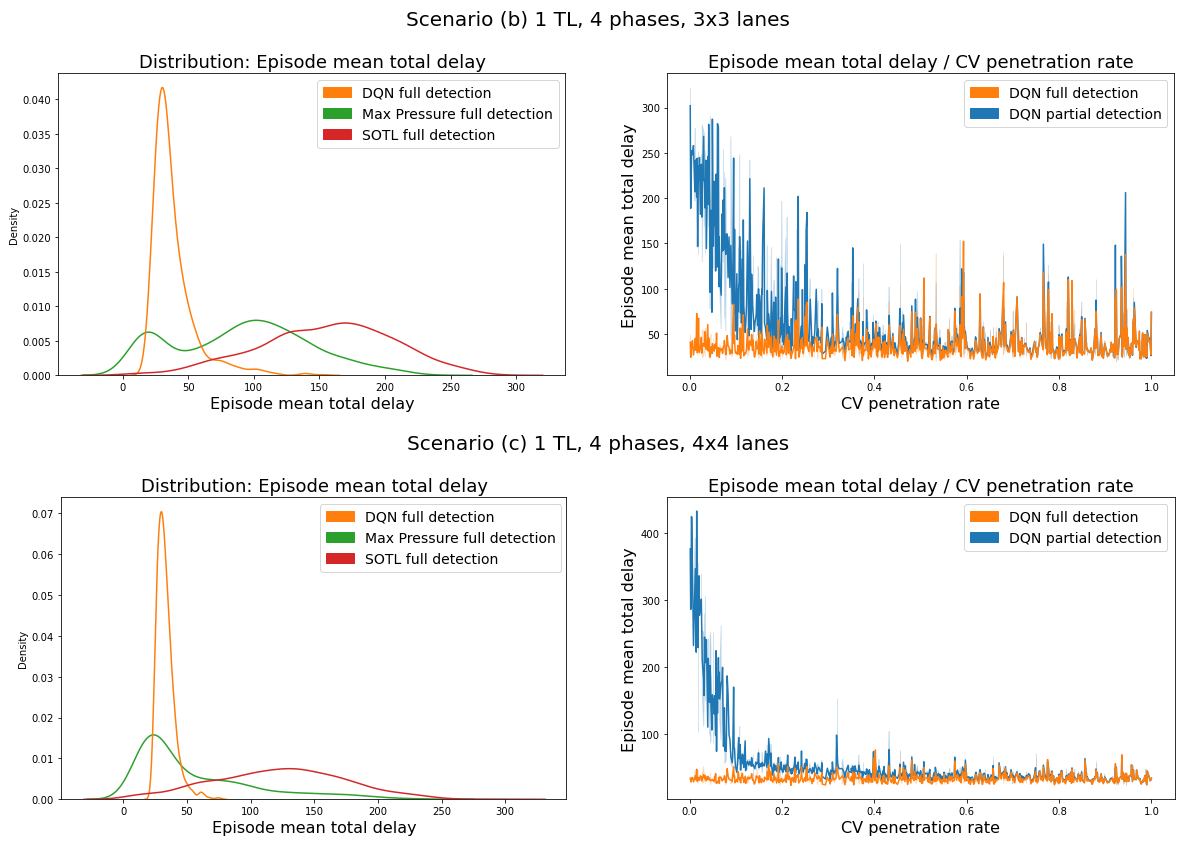
\includegraphics[width=\textwidth]{img/II/analysis_summary.png}
  \centering
  \captionsetup{justification=centering}
  \caption{Excerpts from figures (i) and (iii), for scenarios (b) and (c), and delay KPI.}
\end{figure}

\pagebreak

\subsubsection{Directions for future research}

\textbf{Discussion on limits and improvements} \\
We discuss hereinafter the identified current limits and points of further improvements: 
\begin{enumerate}
\setlength\itemsep{-0.5em}
  \item \textbf{Scenarios}: Here, only five scenarios were tested, all with 4-way intersections. The testing dataset could be diversified with more scenarios, with other network configurations, such as 3-way and 5-way intersections. Additionally, other unexplored road parameters could be included; e.g. prioritized vehicles, 8-phases TL programs, pedestrian crossings, level crossings, taxi services, bus stops, public transports, etc. 
  \item \textbf{Computing power}: Here, both training and testing were performed on an 8-core CPU in limited time. GPU computing could allow to augment the data and results; with (1) faster and longer training, on more difficult scenarios, and with better tuned hyper-parameters, for improved learned policies, and with (2) an expanded testing dataset, enriched both in quantity and quality, for added accuracy in the analysis.
  \item \textbf{Estimation}: Here, we formulated the assumption that information on connected vehicles are precisely known, noting however this statement to be questionable for CV positions due to imprecise infrastructures. Probabilistic estimation methods could be explored and applied to compensate for the uncertainty in measurements.
  \item \textbf{Observation}: Here, we trained a different agent for each new size of partial DTSE. Generalizing partial DTSE across multiple intersection sizes could reduce training time and stabilize performances. An option would be to train the agent on a larger intersection, and apply zero padding in the partial DTSE for smaller intersections.
  \item \textbf{Reward}: Here, we considered the total squared delay, a reward in a fully observable environment that does not allow for post deployment learning, i.e. outside the simulator. An agent with a reward based only on the partial detection of CVs could continue to learn and optimize its policy after being deployed at a real intersection.
  \item \textbf{Low $p_{cv} < 0.2$}: Here, we briefly proposed to handle very low CV penetration rates less than 20\% with a maximum green interval $T_{g,max}$, to simulate a cyclic pre-timed fixed program. This issue of degraded performances remains a major drawback and an obstacle towards usability, and a more efficient solution appears as a necessity.
  \item \textbf{Coordination}: Here, a single agent controls multiple TLs, without coordination and communication. While no significant interference was observed on scenarios (d) and (e), it would probably occur on larger networks. Thus, the model could be adapted to multi agent RL (MARL), for communicating grids of coordinated TLs.
  \item \textbf{Deployment}: Here, the model was deployed only on synthetic road networks in the Sumo simulator. It could be further deployed on real world networks in the simulator, such as the Luxembourg Sumo traffic (LuST) scenario, and, after sufficient validation and within the scope of a controlled experiment, at a real intersection.
\end{enumerate}

Overall, the results obtained before and the points of improvements raised above suggest the presented DQN-ITSCwPD model to be both promising and improvable in many ways. 

\pagebreak

% Conclusion
\section*{Conclusion}
\addcontentsline{toc}{section}{Conclusion}

In this master thesis, we presented the work conducted to address the problematic: \textit{Deep Reinforcement Q-Learning for Intelligent Traffic Signal Control with Partial Detection}.\\

As part of this study and detailed within this report, we proposed two novel contributions: \\

(1) In the first chapter, we presented frameworQ, a python framework for applying deep Q-learning algorithms in customized environments. Aiming at facilitating RL research applications, the algorithms are abstracted from the end users, allowing to generate results faster by putting the focus on designing environments and their action/observation/reward functions, and hyper-parameter tuning; while a set of ready-to-use tools enable to train, test, visualize and compare DQN agents. Four DQN algorithms are implemented; i.e.  vanilla, double, dueling and Per DQN; and combined with further optimizations, e.g. multi-processing training, in the Per3DQN+ algorithm. The proof of concept was demonstrated with two toy customized environments, both achieving expert level performances. \\

(2) In the second chapter, we presented DQN-ITSCwPD, a model for deep Q-learning traffic signal control at single intersections with partial detection over connected vehicles; implemented within frameworQ, with Per3DQN+ and a Sumo customized environment. We introduced a new state representation for partially observable environments, partial DTSE; and a new reward function for TSC, total squared delay. Additionally, we provided tuned values for the convolutional dueling DQN architecture and the hyper-parameters. The model was evaluated against two existing actuated TSC algorithms, Max Pressure and SOTL, in a two-step comparative analysis on four traffic key performance indicators. As a result, we concluded the model to be more efficient than the baselines for 4-phases TL programs in full detection, and estimated partial detection performance thresholds for CV penetration rates, with acceptability at $p_{cv} \in [0.2,0.3]$ and optimality at $p_{cv} \in [0.4,0.5]$. \\

Lastly, on a personal note, this project was for me the opportunity to explore a research topic, practice the research methodology and acquire skills to pursue research activities.
During this internship, I learned to formalise a research problematic, and to identify the adequate literature and tools to address it. I also learned to read and reproduce scientific papers in depth, and implement complex models, algorithms and methods. Furthermore, I learned to perform numerical tests and experiments to evaluate propositions and estimate performances against benchmarks. And most of all, I learned to lead a project, for which I have been entrusted with the responsibility and autonomy, from the beginning to the end. \\

I would like to thank my supervisor, Dr. Nadir Farhi, and the team at GRETTIA, UGE.

\pagebreak


% Conclusion
\section*{Appendix}
\addcontentsline{toc}{section}{Appendix}

\subsection*{Appendix 1, Results (2.3.1) Scenarios: Sumo visuals}
\addcontentsline{toc}{subsection}{Appendix 1, Results (2.3.1) Scenarios: Sumo visuals}

This appendix contains the Sumo visuals for the traffic scenarios presented in part 2.3.1. \\

\begin{figure}[h]
\subsubsection*{(a): 1 traffic light, 2 phases, 2x2 incoming lanes.}
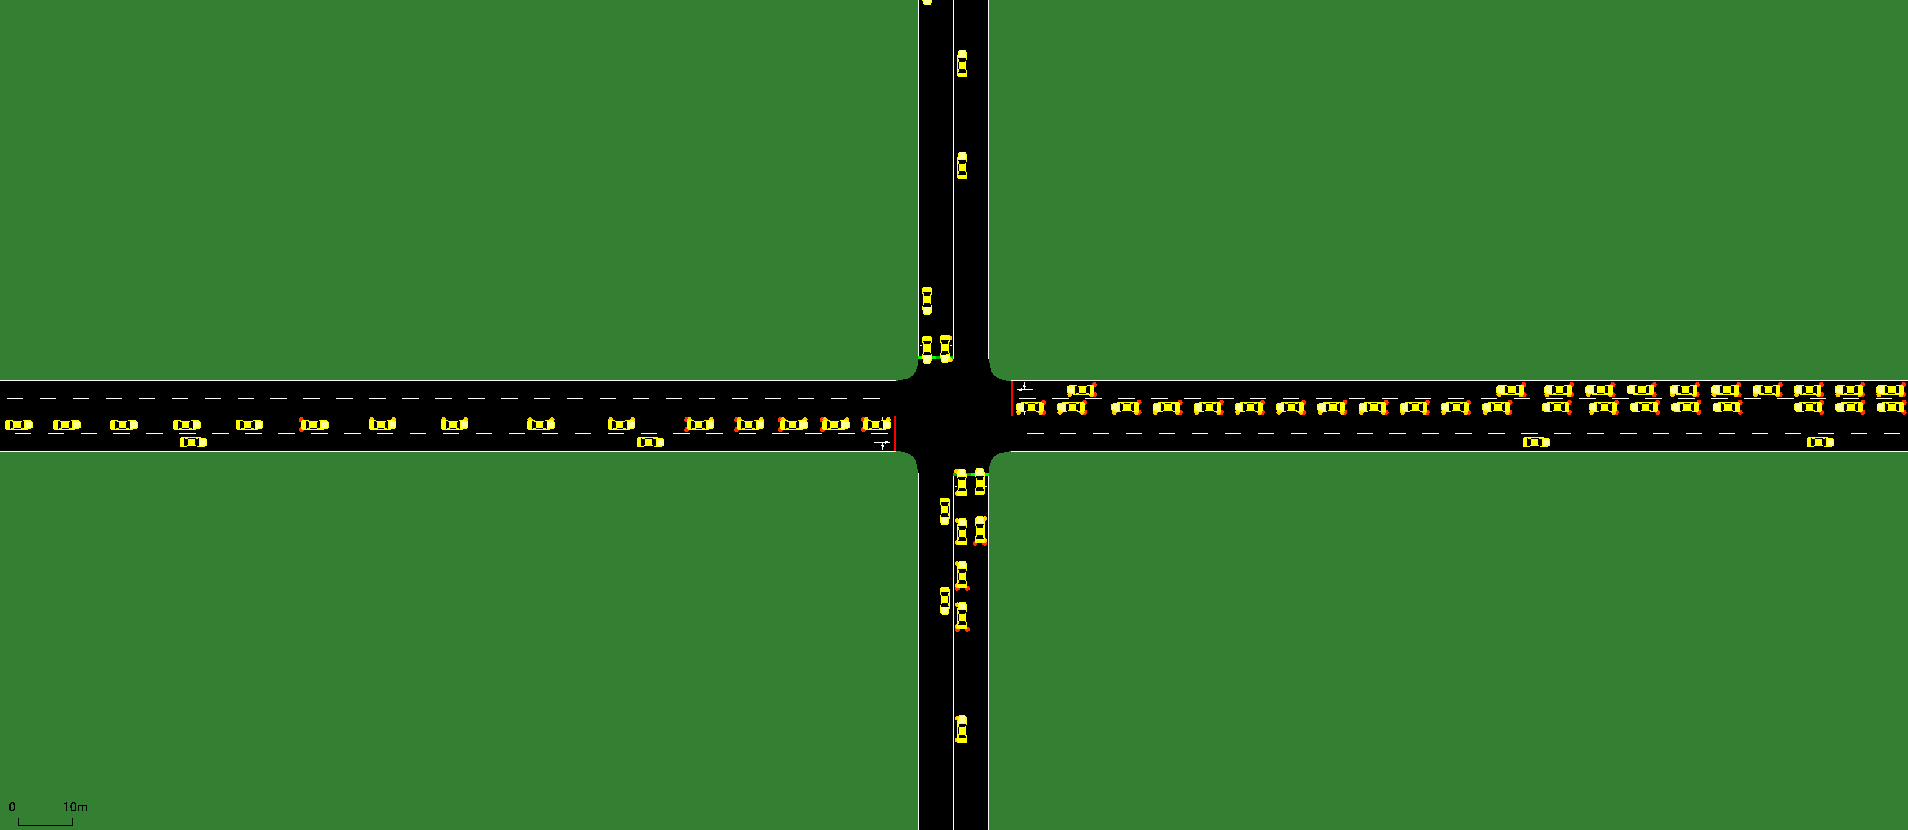
\includegraphics[width=\textwidth]{img/Appendix/scenario_a.png}
\centering
\end{figure}

\begin{figure}[h]
\subsubsection*{(b): 1 traffic light, 4 phases, 3x3 incoming lanes.}
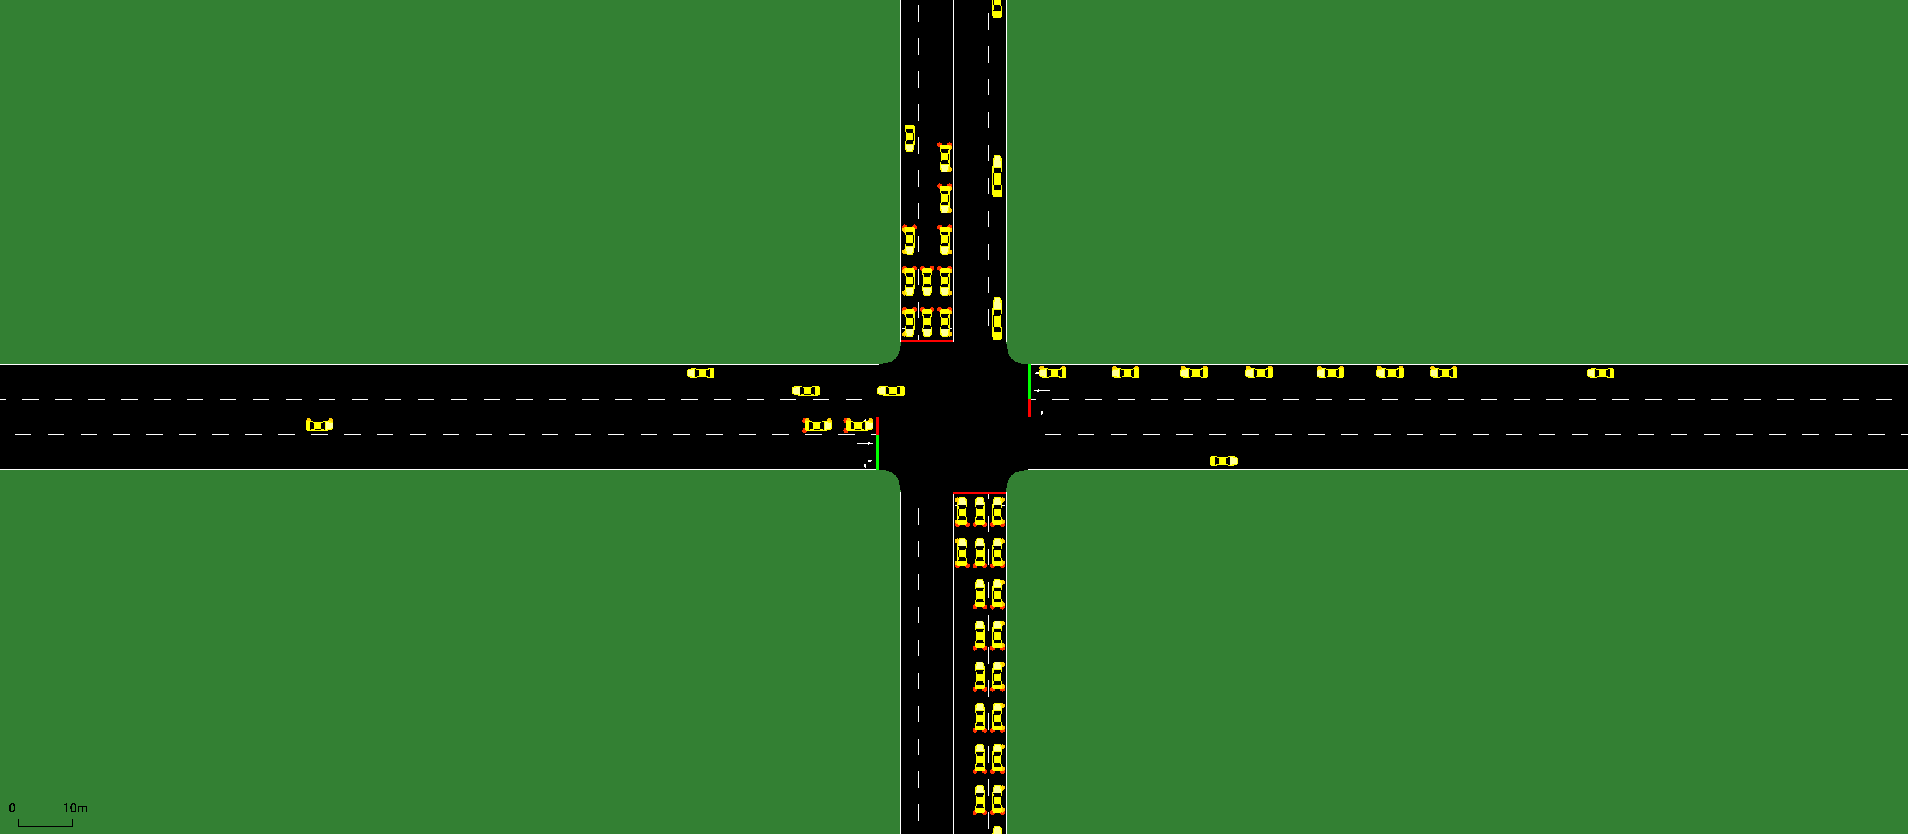
\includegraphics[width=\textwidth]{img/Appendix/scenario_b.png}
\centering
\end{figure}

\pagebreak

\newgeometry{left= 3cm, right= 2cm, bottom= 0cm, top= 2.6cm}

\begin{figure}[h]
\subsubsection*{(c): 1 traffic light, 4 phases, 4x4 incoming lanes.}
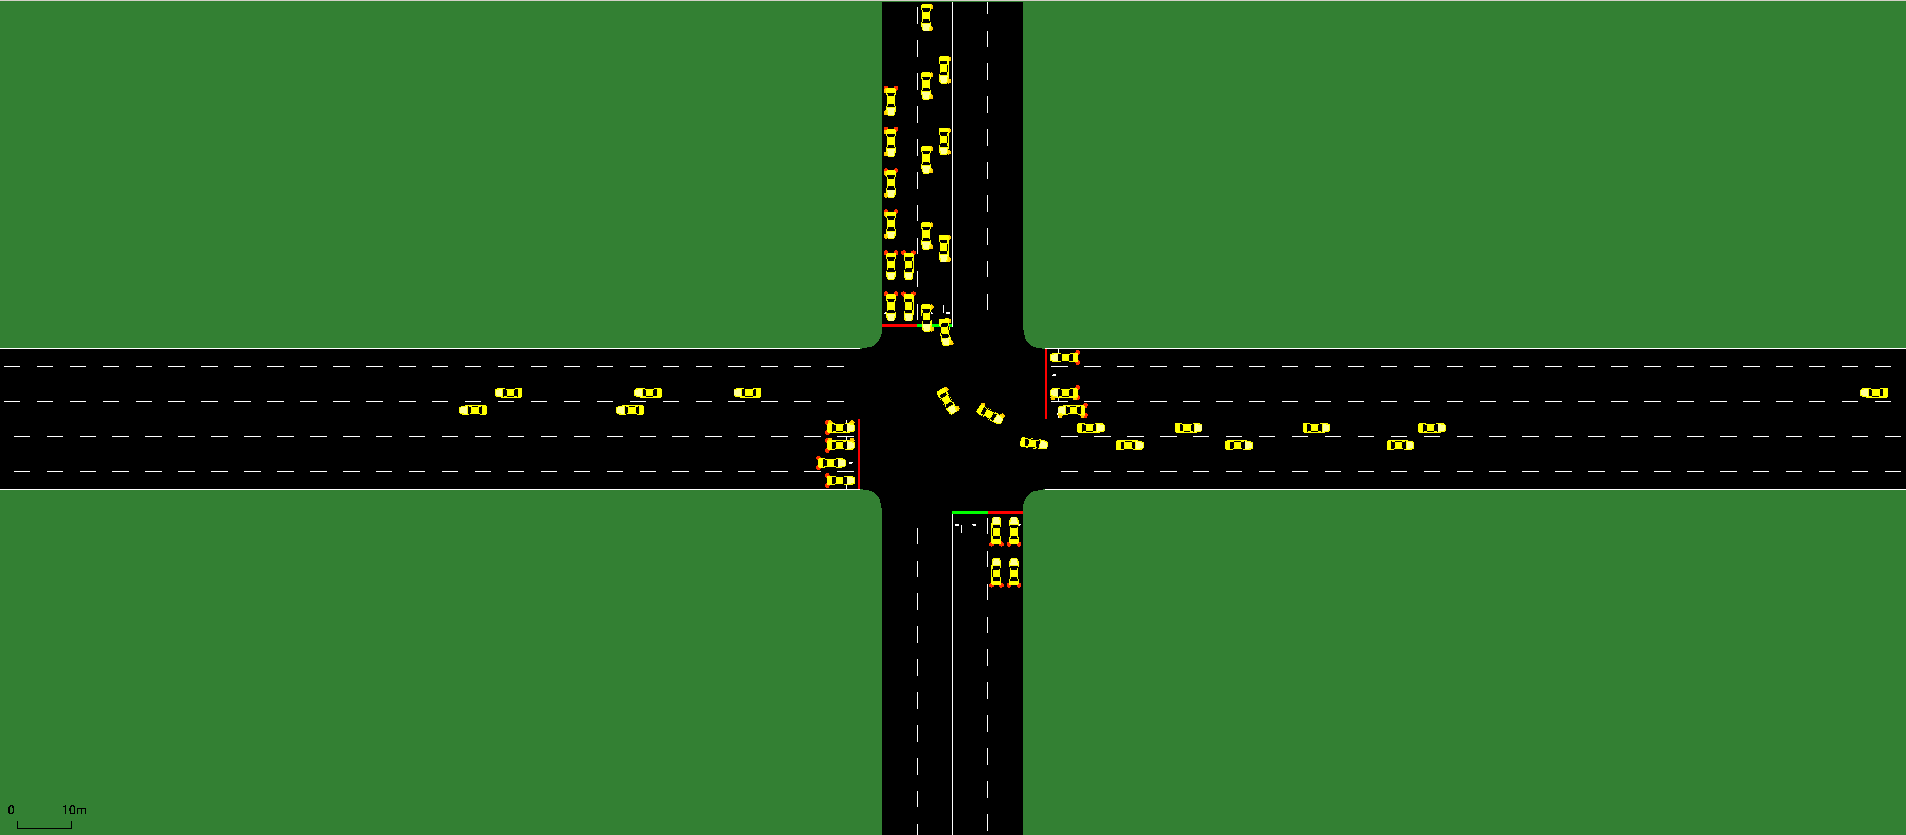
\includegraphics[width=\textwidth]{img/Appendix/scenario_c.png}
\centering
\end{figure}

\begin{figure}[h]
\subsubsection*{(d): 2 traffic lights, 4 phases, 3x3 incoming lanes.}
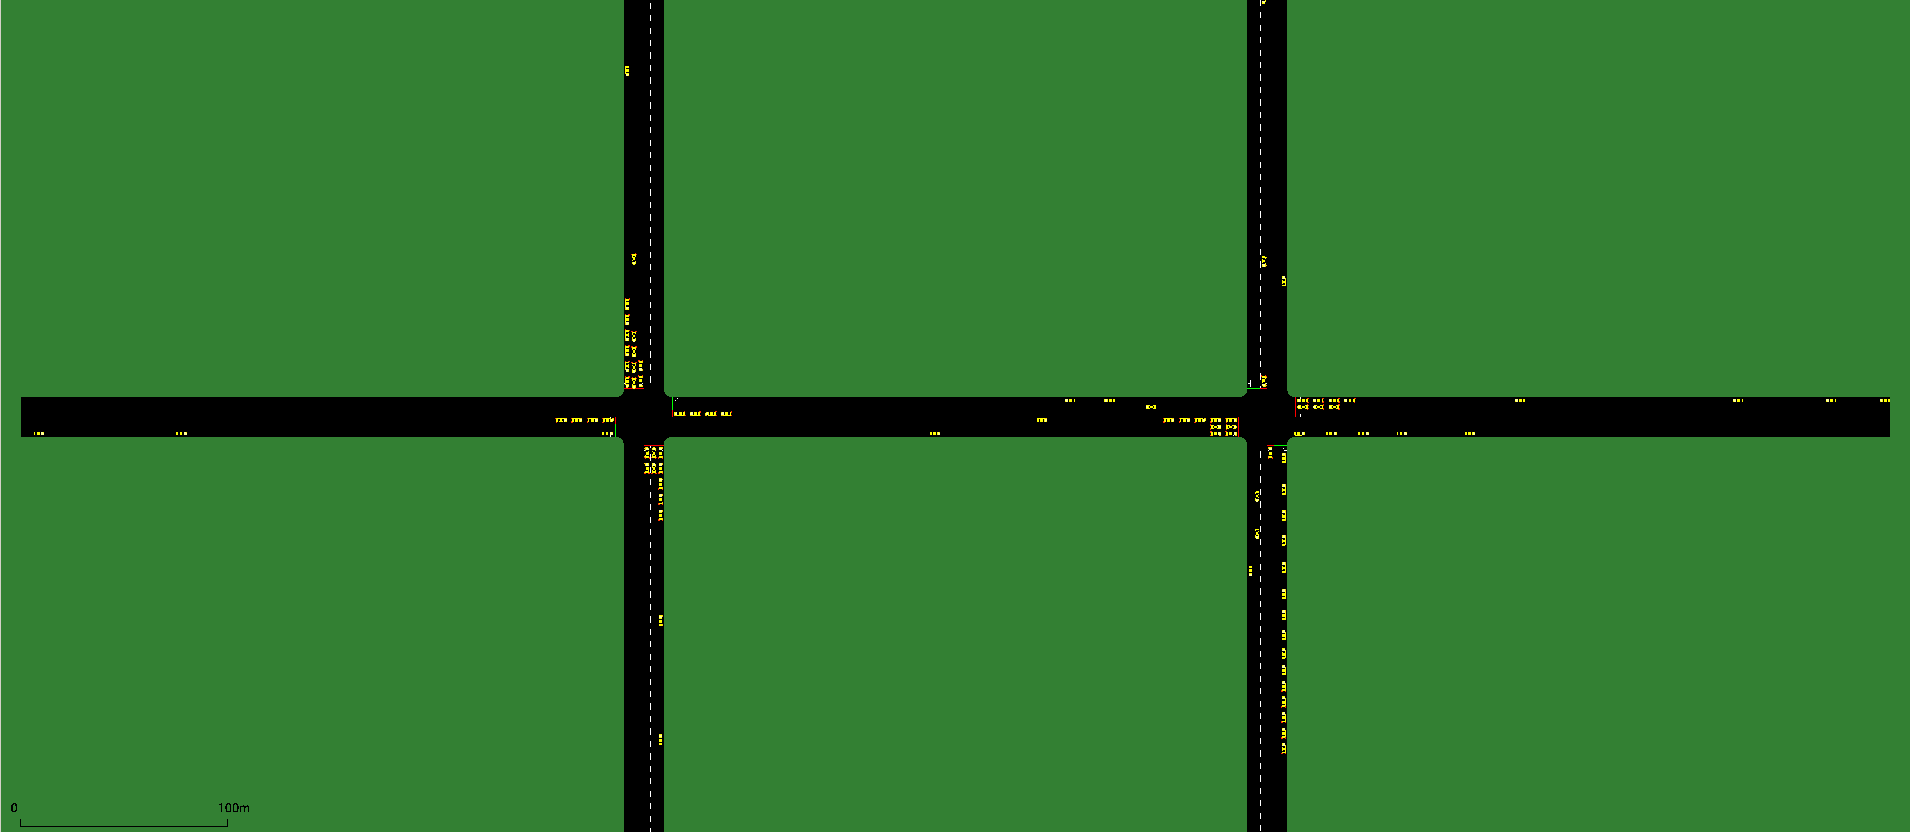
\includegraphics[width=\textwidth]{img/Appendix/scenario_d.png}
\centering
\end{figure}

\begin{figure}[h!]
\subsubsection*{(e): 4 traffic lights, 4 phases, 3x3 incoming lanes.}
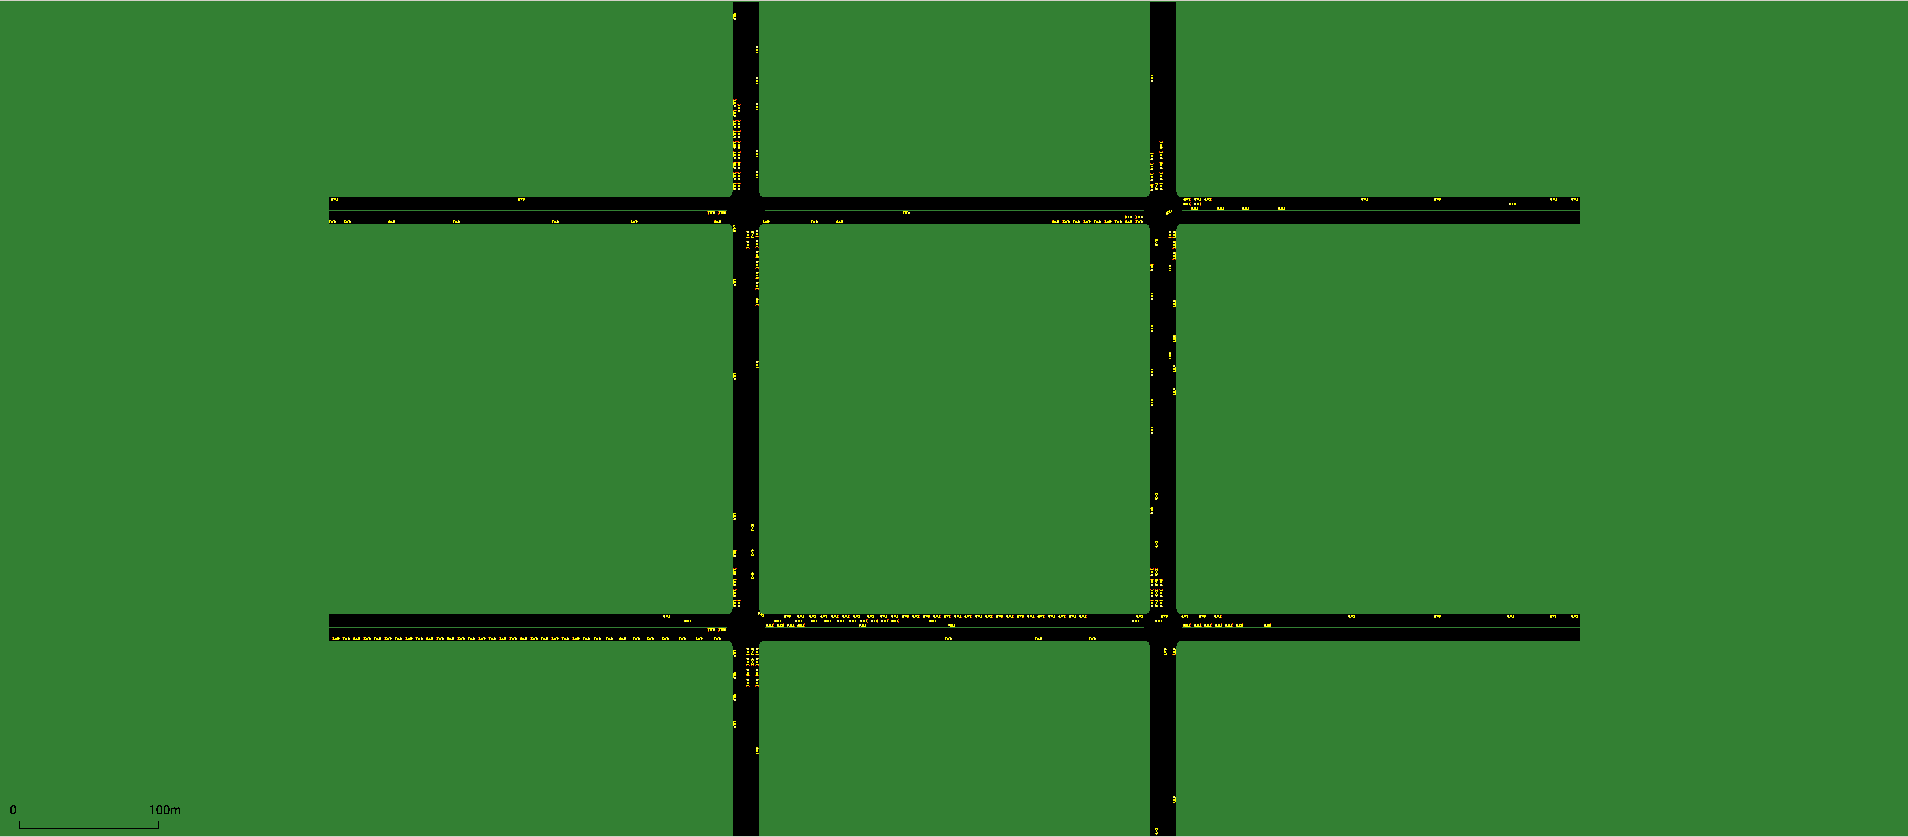
\includegraphics[width=\textwidth]{img/Appendix/scenario_e.png}
\centering
\end{figure}

\restoregeometry

\pagebreak

\subsection*{Appendix 2, Results (2.3.2) Analysis: figures, tables}
\addcontentsline{toc}{subsection}{Appendix 2, Results (2.3.2) Analysis: figures, tables}

This appendix contains the complete results for the DQN-ITSCwPD project, i.e. figures and tables, discussed in part 2.3.2.
Hereafter are the legends of following figures and tables: \\

\textbf{- 4 KP indicators:} \\
For all vehicles in all incoming lanes, the mean over one episode and the TLs of the total: 
\begin{enumerate}
    \setlength\itemsep{-0.5em}
    \item \textbf{Episode mean total accumulated waiting time}: accumulated waiting time;
    \item \textbf{Episode mean total delay}: delay;
    \item \textbf{Episode mean total queue length}: queue length;
    \item \textbf{Episode mean total volume}: volume.
\end{enumerate}

\textbf{- Traffic scenarios:} 
\begin{itemize}
    \setlength\itemsep{-0.5em}
    \item \textbf{(a)}: 1 traffic light, 2 phases, 2x2 incoming lanes;
    \item \textbf{(b)}: 1 traffic light, 4 phases, 3x3 incoming lanes;
    \item \textbf{(c)}: 1 traffic light, 4 phases, 4x4 incoming lanes;
    \item \textbf{(d)}: 2 traffic lights, 4 phases, 3x3 incoming lanes;
    \item \textbf{(e)}: 4 traffic lights, 4 phases, 3x3 incoming lanes.
\end{itemize}

\textbf{- Figure colors:}
\begin{itemize}
    \setlength\itemsep{-0.5em}
    \item \textbf{Blue}: DQN partial detection (DQN PD);
    \item \textbf{Orange}: DQN full detection (DQN FD);
    \item \textbf{Green}: Max Pressure full detection (MP FD);
    \item \textbf{Red}: SOTL full detection (SOTL FD);
    \item \textbf{Purple, brown, pink, grey, khaki}: scenarios (a), (b), (c), (d), (e).
\end{itemize}

\pagebreak

\newgeometry{left= 0.75cm, right= 0.75cm, bottom= 0cm, top= 0cm}
\begin{figure}[h]
\subsubsection*{(i, 1/3) Comparison of density distributions for full detection DQN, Max Pressure and SOTL; by 4 KPIs, and by scenario, and over 1000 episodes.}
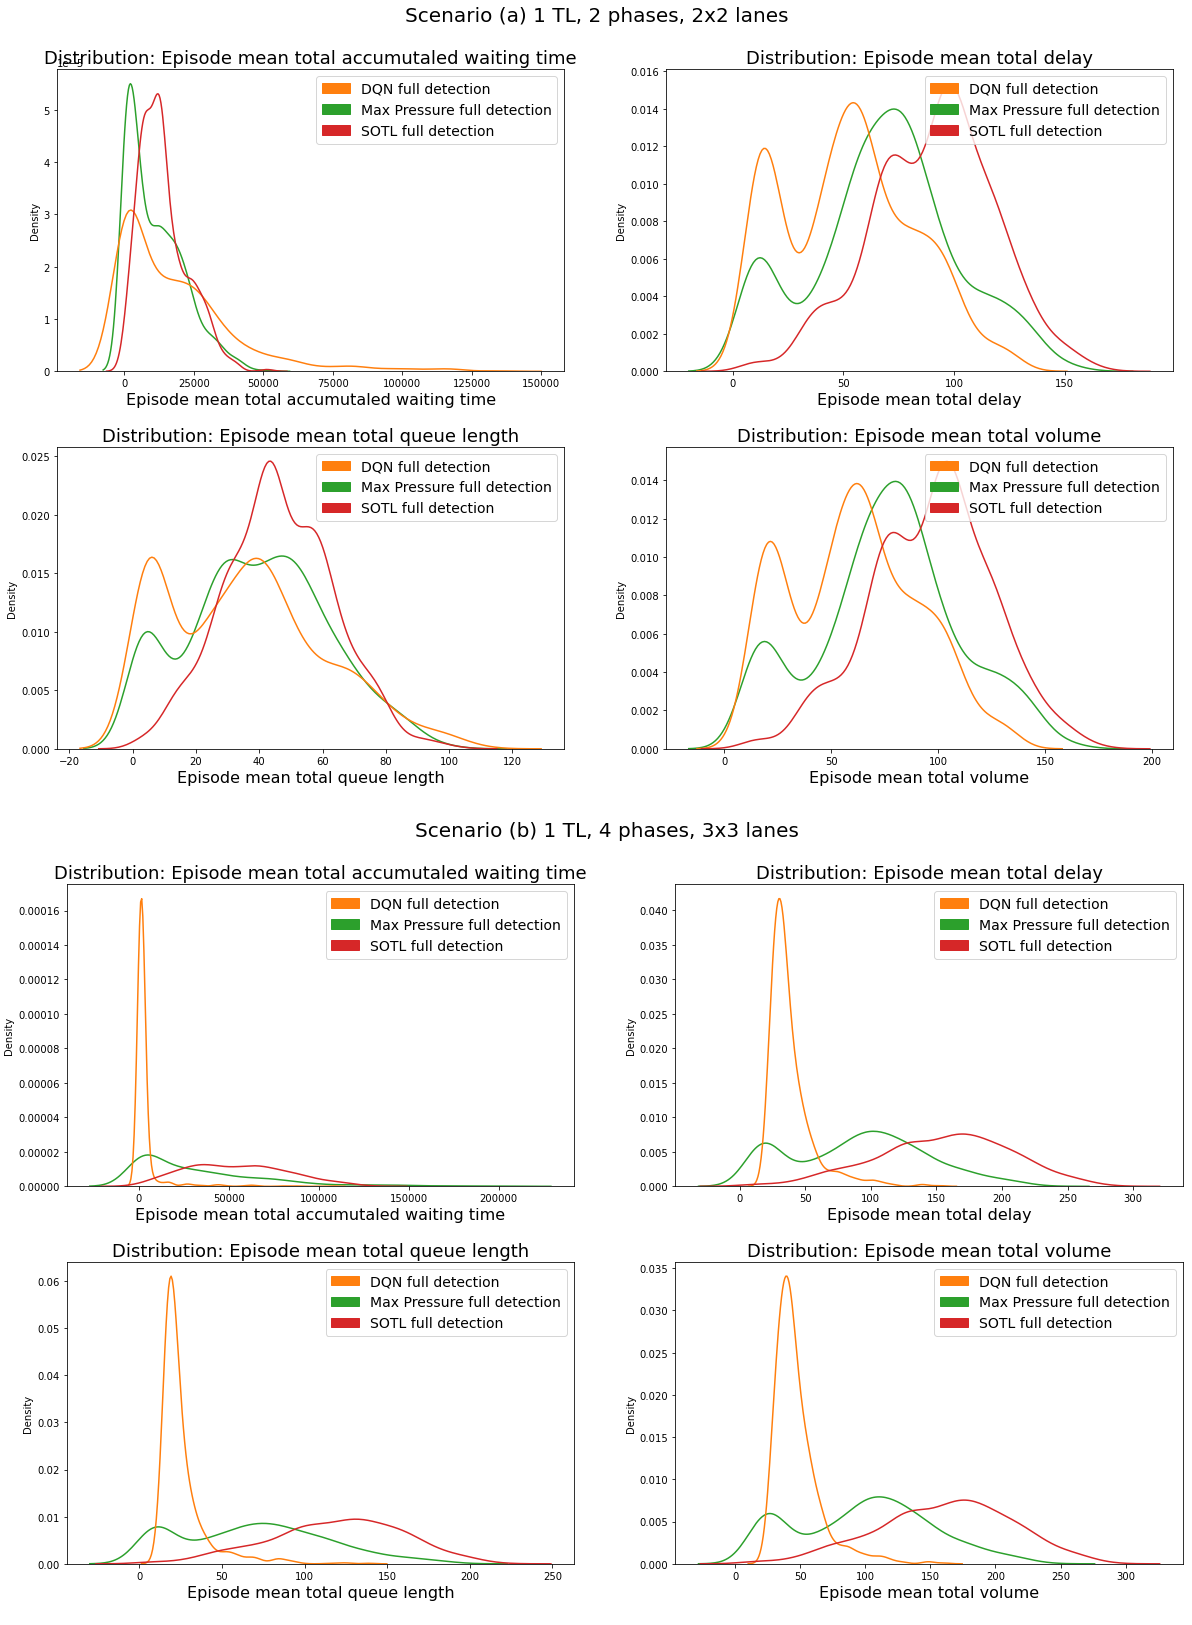
\includegraphics[width=\textwidth]{img/Appendix/1_1-2.png}
\centering
\end{figure}
\restoregeometry

\pagebreak

\newgeometry{left= 0.75cm, right= 0.75cm, bottom= 0cm, top= 0cm}
\begin{figure}[h]
\subsubsection*{(i, 2/3)}
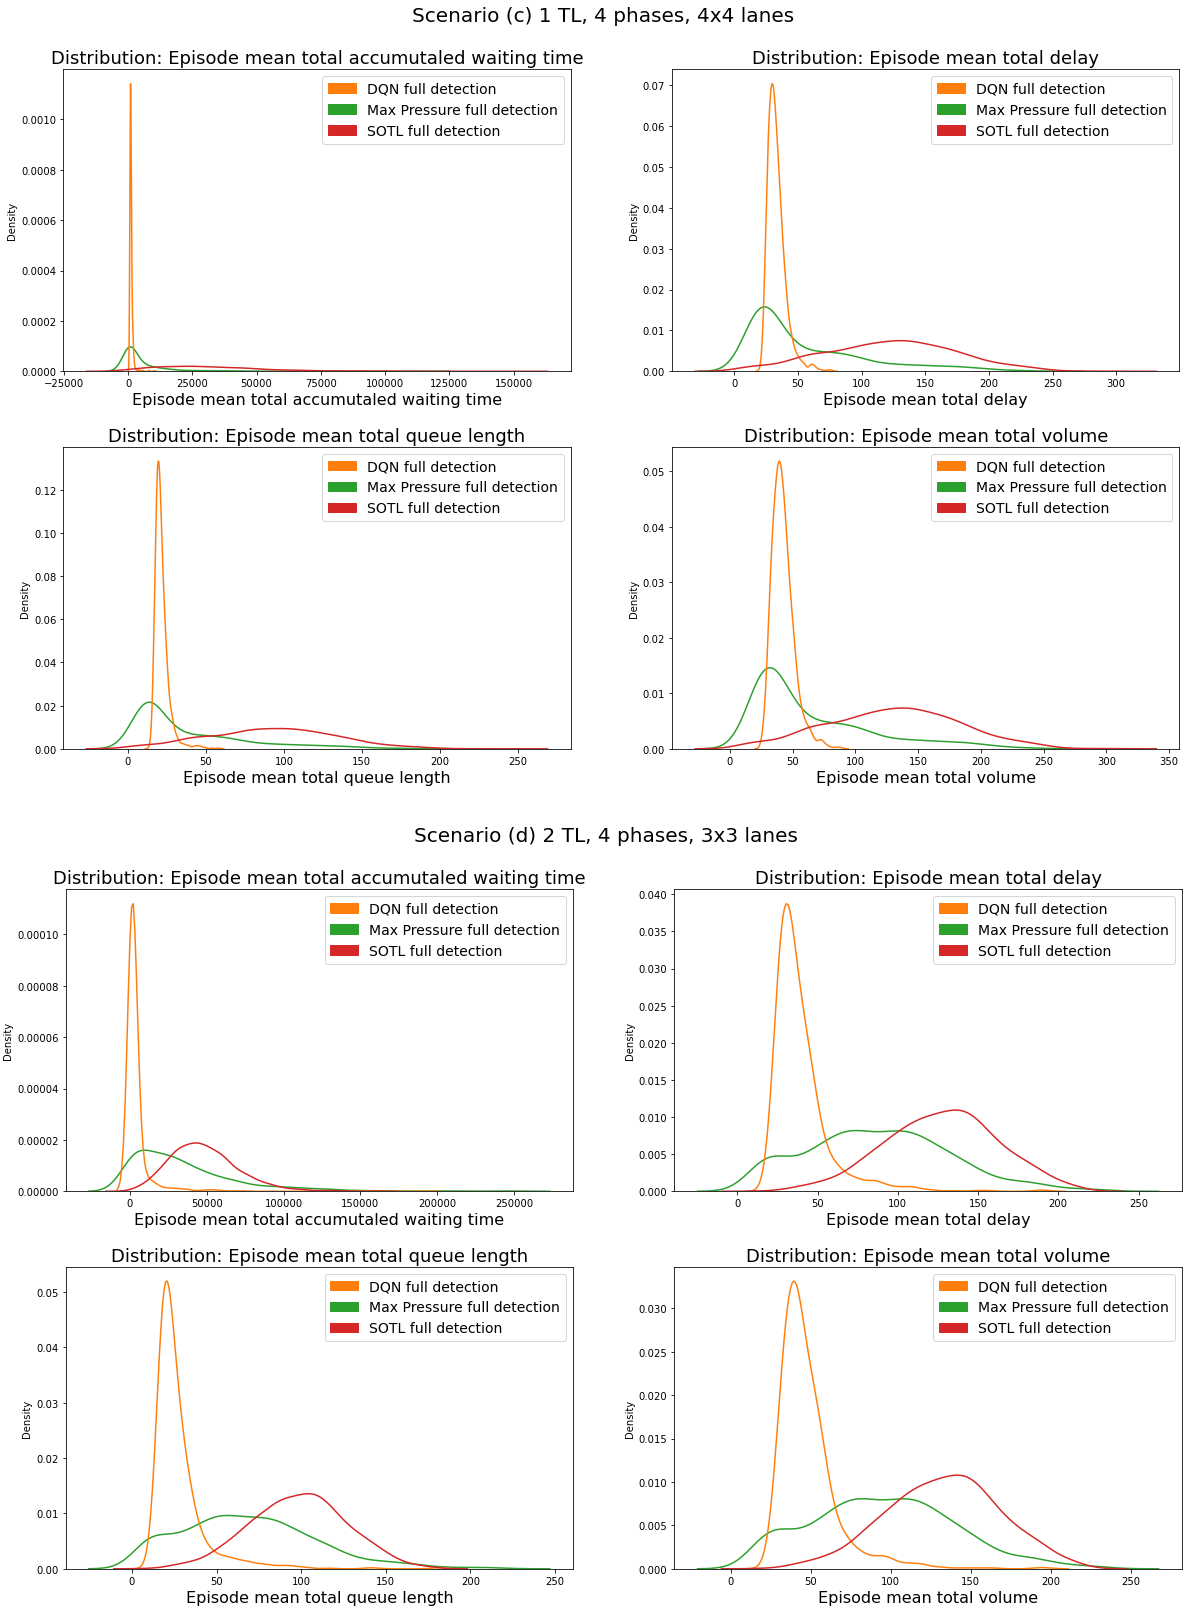
\includegraphics[width=\textwidth]{img/Appendix/1_3-4.png}
\centering
\end{figure}
\restoregeometry

\pagebreak

\newgeometry{left= 0.75cm, right= 0.75cm}
\begin{figure}[h]
\subsubsection*{(i, 3/3)}
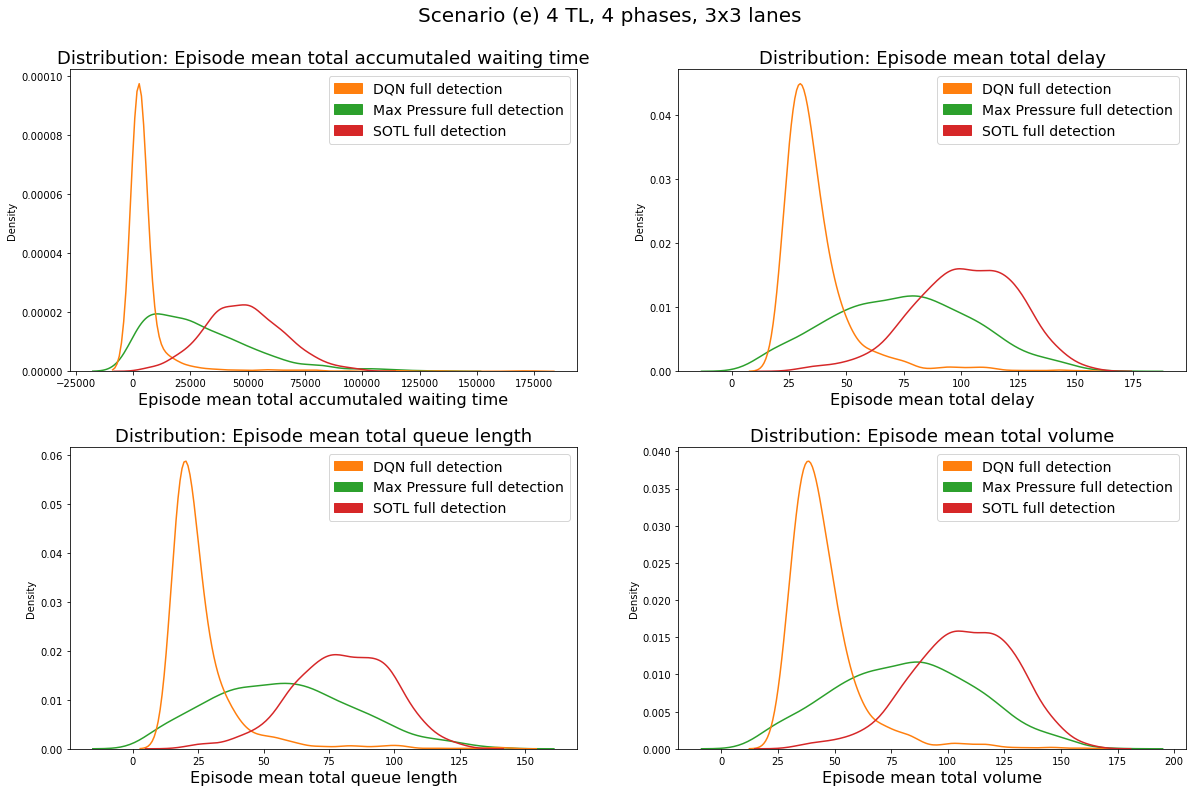
\includegraphics[width=\textwidth]{img/Appendix/1_5.png}
\centering
\end{figure}
\restoregeometry

\pagebreak

\newgeometry{left= 0.75cm, right= 0.75cm}
\begin{figure}[h]
\subsubsection*{(ii, 1/2) Comparison of statistics of 4 KPIs for full detection DQN, Max Pressure and SOTL; by scenario, and by mean, median, first quartile, third quartile, variance and standard deviation, and over 1000 episodes.}
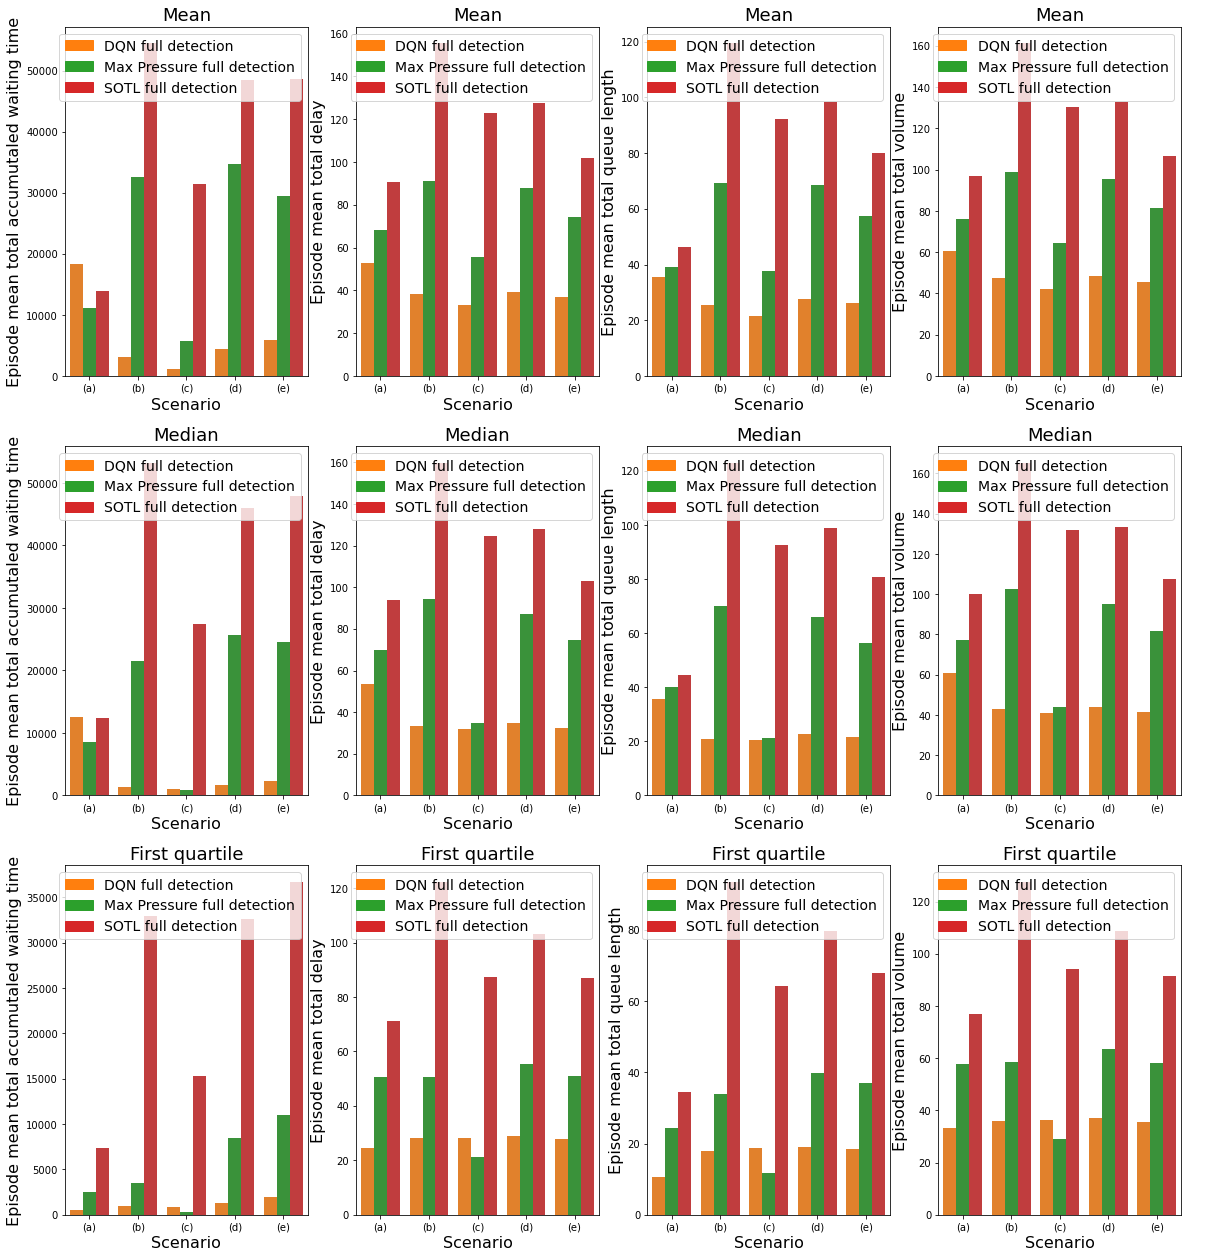
\includegraphics[width=\textwidth]{img/Appendix/2_1.png}
\centering
\end{figure}
\restoregeometry

\pagebreak

\newgeometry{left= 0.75cm, right= 0.75cm}
\begin{figure}[h]
\subsubsection*{(ii, 2/2)}
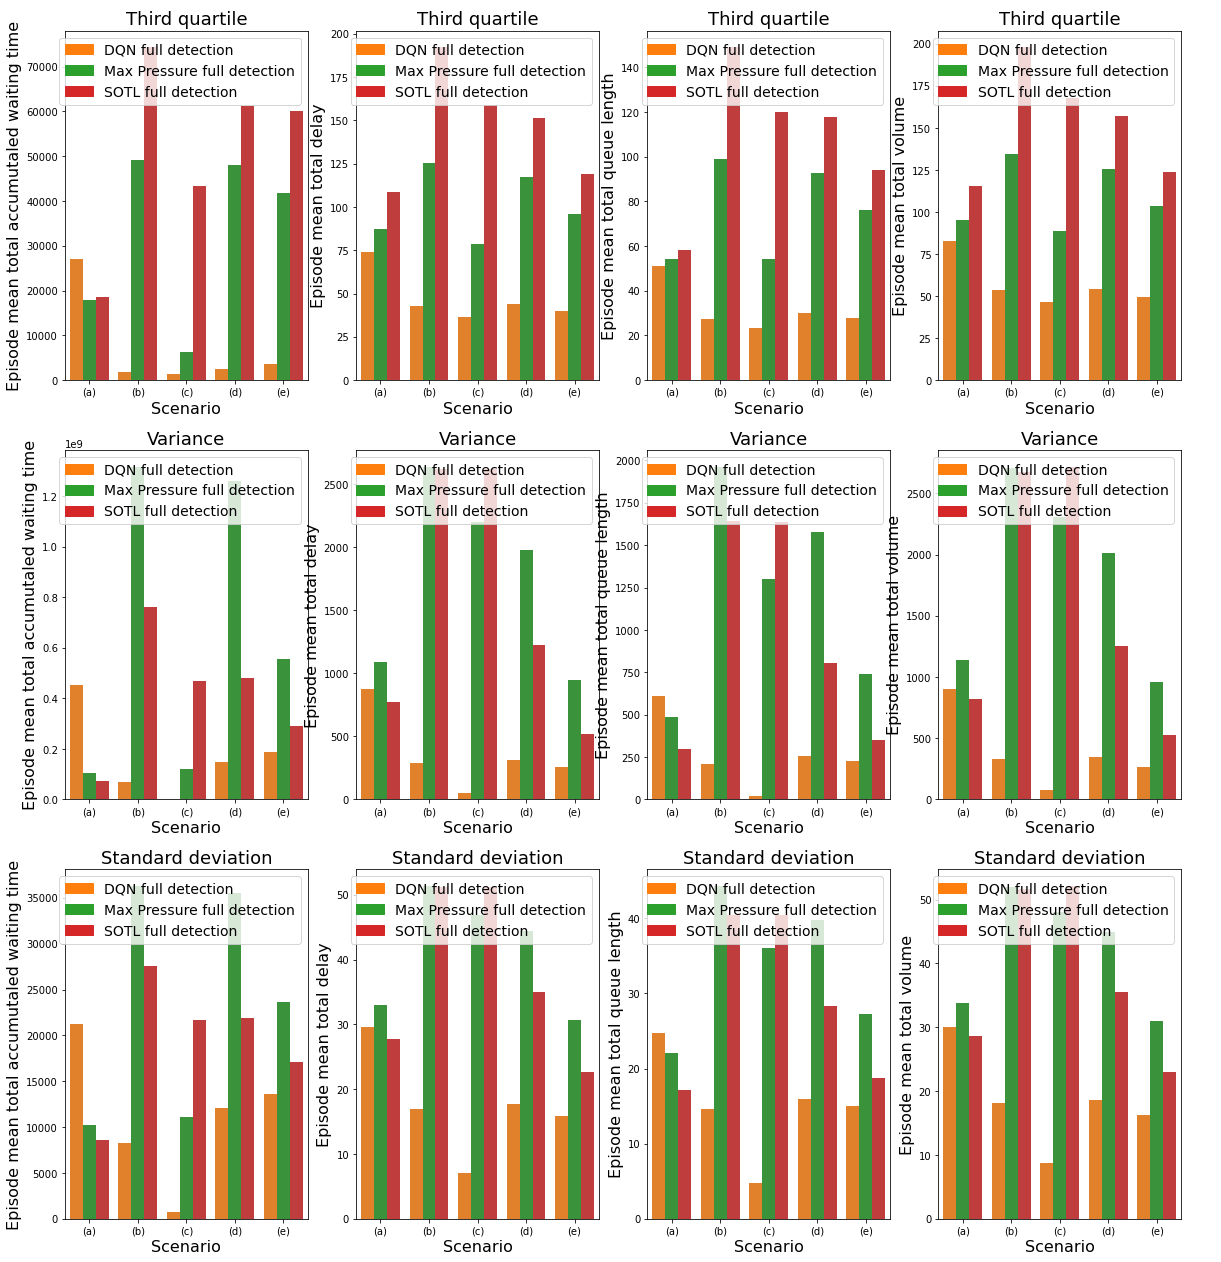
\includegraphics[width=\textwidth]{img/Appendix/2_2.png}
\centering
\end{figure}
\restoregeometry

\pagebreak

\newgeometry{left= 0.75cm, right= 0.75cm, bottom= 0cm, top= 0cm}
\begin{figure}[h]
\subsubsection*{(iii, 1/3) Comparison of 4 KPIs for full detection DQN and partial detection DQN; by penetration rate of connected vehicles, and by scenario, and over 1000 episodes.}
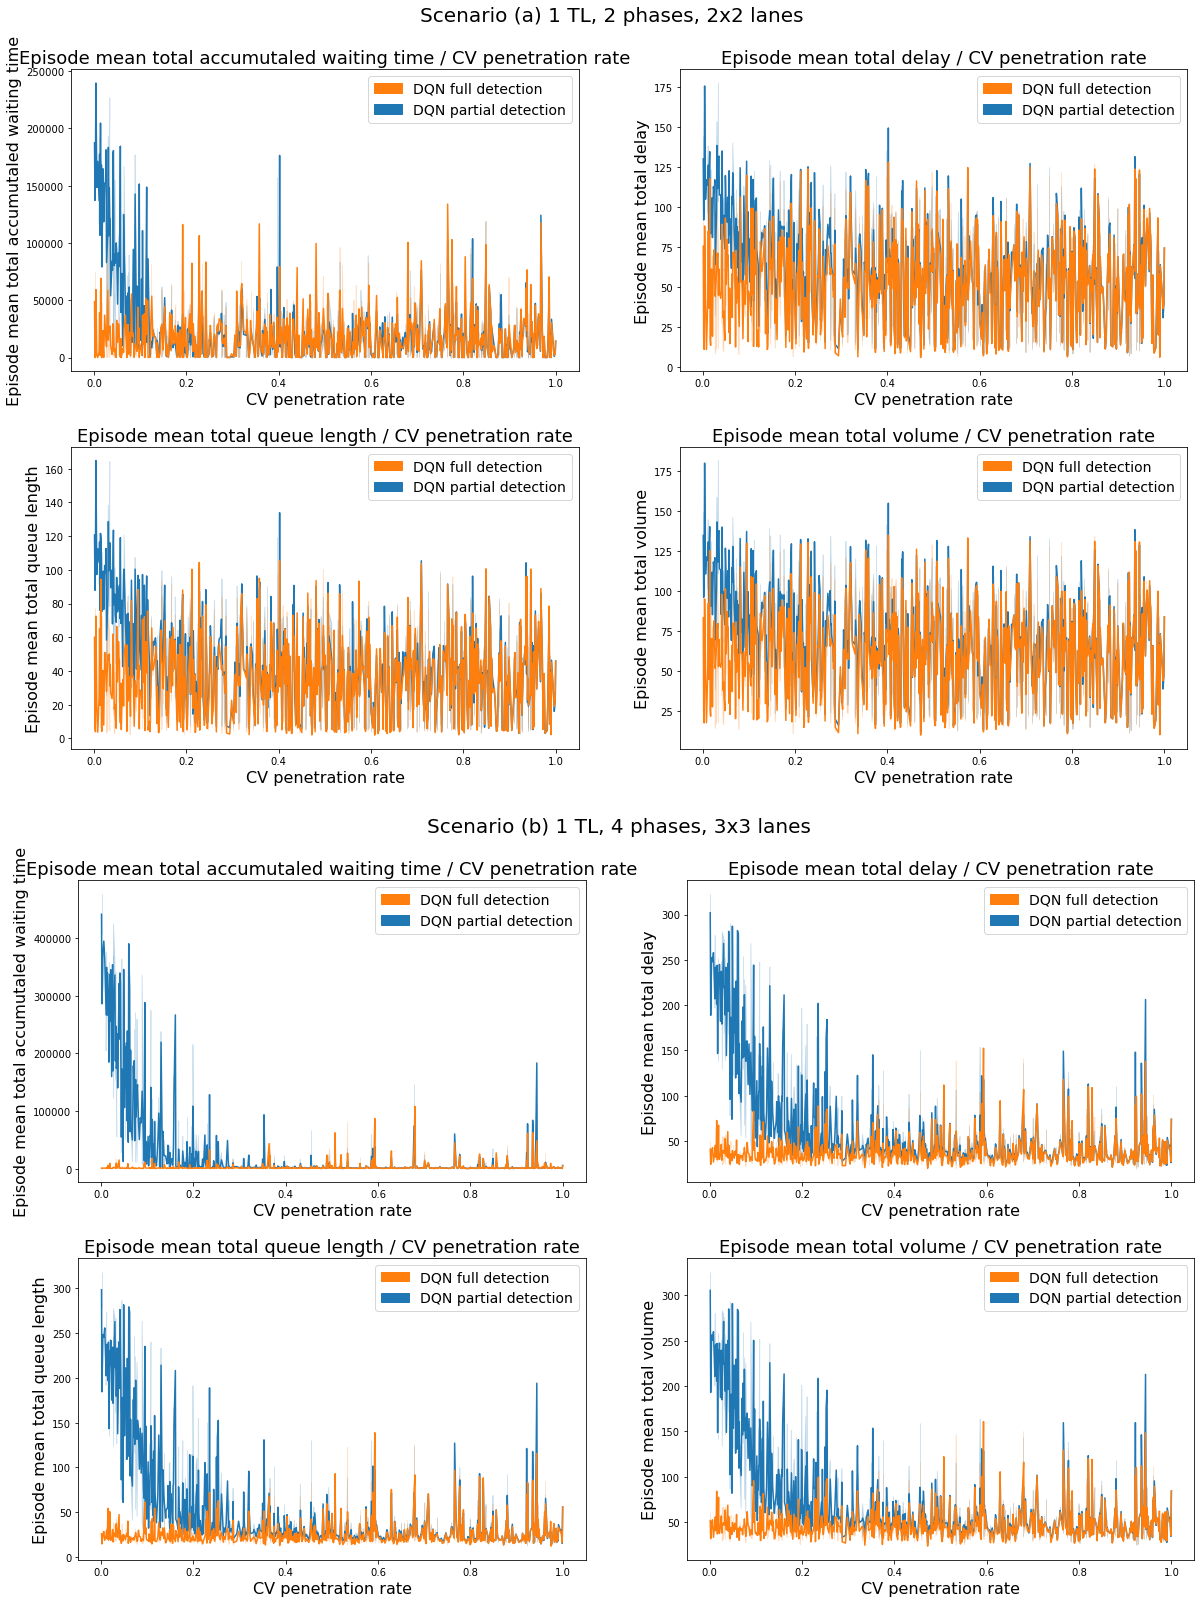
\includegraphics[width=\textwidth]{img/Appendix/3_1-2.png}
\centering
\end{figure}
\restoregeometry

\pagebreak

\newgeometry{left= 0.75cm, right= 0.75cm, bottom= 0cm, top= 0cm}
\begin{figure}[h]
\subsubsection*{(iii, 2/3)}
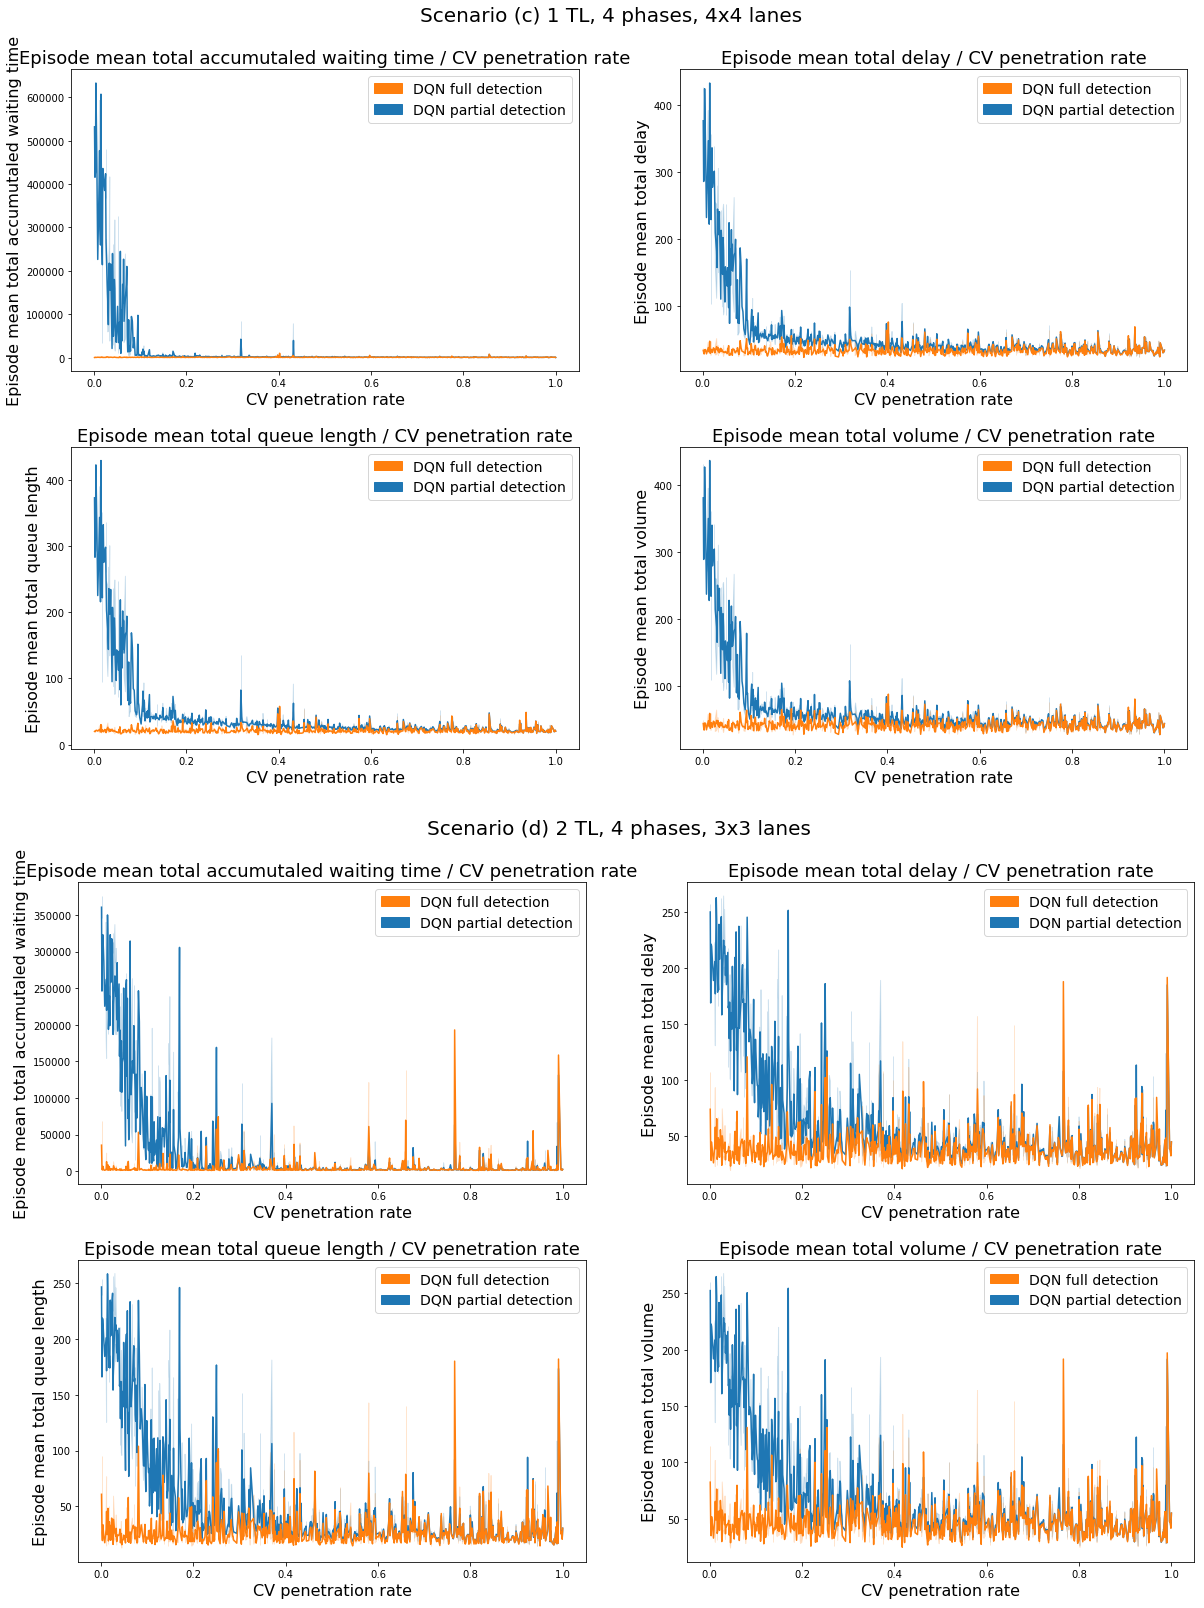
\includegraphics[width=\textwidth]{img/Appendix/3_3-4.png}
\centering
\end{figure}
\restoregeometry

\pagebreak

\newgeometry{left= 0.75cm, right= 0.75cm}
\begin{figure}[h]
\subsubsection*{(iii, 3/3)}
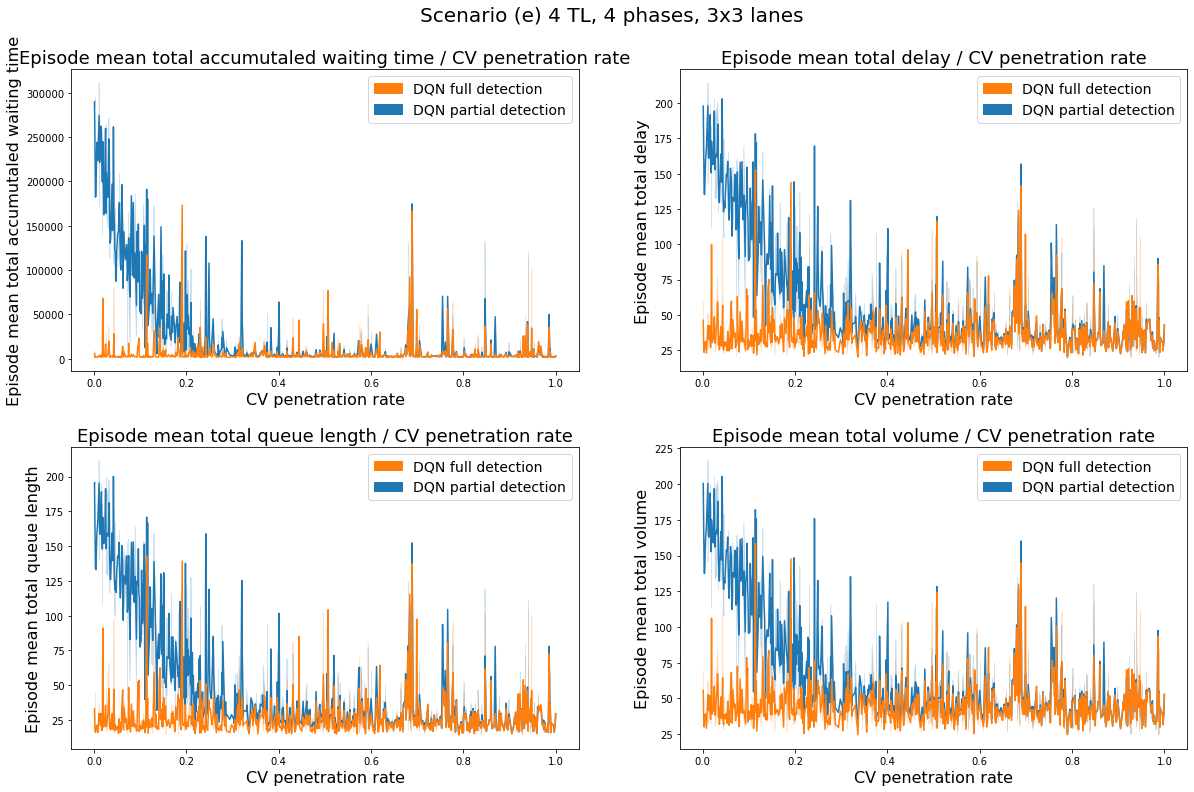
\includegraphics[width=\textwidth]{img/Appendix/3_5.png}
\centering
\end{figure}
\subsubsection*{(iv, 1/1) Comparison of percentage loss between full detection DQN and partial detection DQN of 4 KPIs for all scenarios; by range of penetration rates of connected vehicles, and over 1000 episodes.}
\restoregeometry

\pagebreak

\newgeometry{left= 0.75cm, right= 0.75cm, bottom= 0cm, top= 0cm}
\begin{figure}[h]
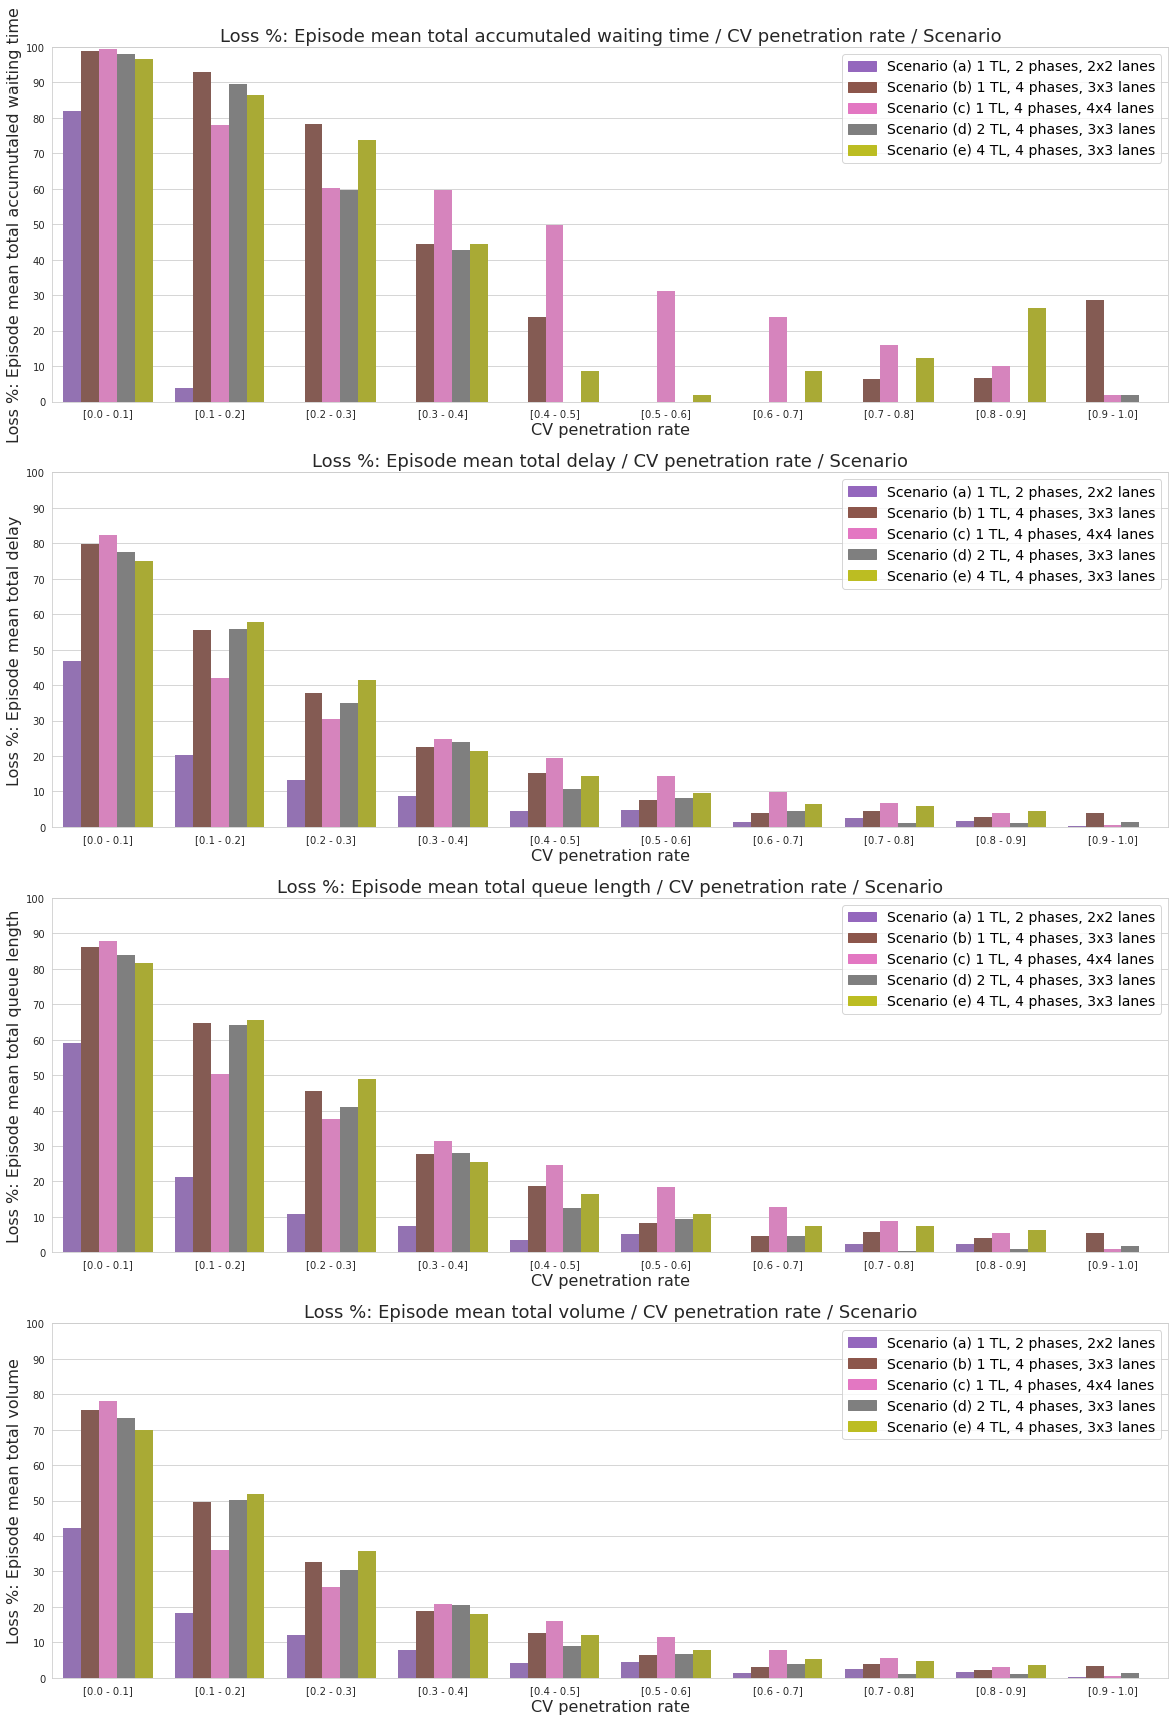
\includegraphics[width=\textwidth]{img/Appendix/4.png}
\centering
\end{figure}
\restoregeometry

\pagebreak

\subsubsection*{(v, 1/3) Table of numerical results for (ii). \\
(Comparison of statistics of 4 KPIs for full detection DQN, Max Pressure and SOTL; by scenario, and by mean, median, first quartile, third quartile, variance and standard deviation, and over 1000 episodes.)}

\begin{table}[htbp]
\centering
\setlength\tabcolsep{2pt}
\begin{tabular}{|c|c|}
\hline
Column &                                                           Title \\
\hline
     A &                                                        Scenario \\
     B &                                                       Algorithm \\
     C &               Mean: Episode mean total accumutaled waiting time \\
     D &                                  Mean: Episode mean total delay \\
     E &                           Mean: Episode mean total queue length \\
     F &                                 Mean: Episode mean total volume \\
     G &             Median: Episode mean total accumutaled waiting time \\
     H &                                Median: Episode mean total delay \\
     I &                         Median: Episode mean total queue length \\
     J &                               Median: Episode mean total volume \\
     K &     First quartile: Episode mean total accumutaled waiting time \\
     L &                        First quartile: Episode mean total delay \\
     M &                 First quartile: Episode mean total queue length \\
     N &                       First quartile: Episode mean total volume \\
     O &     Third quartile: Episode mean total accumutaled waiting time \\
     P &                        Third quartile: Episode mean total delay \\
     Q &                 Third quartile: Episode mean total queue length \\
     R &                       Third quartile: Episode mean total volume \\
     S &           Variance: Episode mean total accumutaled waiting time \\
     T &                              Variance: Episode mean total delay \\
     U &                       Variance: Episode mean total queue length \\
     V &                             Variance: Episode mean total volume \\
     W & Standard deviation: Episode mean total accumutaled waiting time \\
     X &                    Standard deviation: Episode mean total delay \\
     Y &             Standard deviation: Episode mean total queue length \\
     Z &                   Standard deviation: Episode mean total volume \\
\hline
\end{tabular}
\end{table}

\pagebreak

\newgeometry{left= 0cm, right= 0cm, bottom= 0cm, top= 0cm}

\begin{table}[htbp]
\centering
\small
\setlength\tabcolsep{2pt}
\begin{tabular}{|c|c|c|c|c|c|c|c|c|c|c|c|c|c|}
\hline
{} &    A &          B &       C &     D &     E &     F &       G &     H &     I &     J &       K &     L &    M \\
\hline
0  &  (a) &   DQN (FD) & 18280.2 &  52.8 &  35.7 &  60.6 & 12542.0 &  53.3 &  35.7 &  61.1 &   475.1 &  24.6 & 10.6 \\
1  &  (a) &    MP (FD) & 11130.9 &  68.1 &  39.3 &  76.0 &  8528.5 &  69.8 &  40.0 &  77.4 &  2543.0 &  50.4 & 24.5 \\
2  &  (a) &  SOTL (FD) & 13864.7 &  90.5 &  46.2 &  96.8 & 12433.5 &  94.0 &  44.6 & 100.0 &  7325.2 &  71.3 & 34.4 \\
3  &  (a) &   DQN (FD) & 18280.2 &  52.8 &  35.7 &  60.6 & 12542.0 &  53.3 &  35.7 &  61.1 &   475.1 &  24.6 & 10.6 \\
4  &  (a) &    MP (FD) & 11130.9 &  68.1 &  39.3 &  76.0 &  8528.5 &  69.8 &  40.0 &  77.4 &  2543.0 &  50.4 & 24.5 \\
5  &  (a) &  SOTL (FD) & 13864.7 &  90.5 &  46.2 &  96.8 & 12433.5 &  94.0 &  44.6 & 100.0 &  7325.2 &  71.3 & 34.4 \\
6  &  (a) &   DQN (FD) & 18280.2 &  52.8 &  35.7 &  60.6 & 12542.0 &  53.3 &  35.7 &  61.1 &   475.1 &  24.6 & 10.6 \\
7  &  (a) &    MP (FD) & 11130.9 &  68.1 &  39.3 &  76.0 &  8528.5 &  69.8 &  40.0 &  77.4 &  2543.0 &  50.4 & 24.5 \\
8  &  (a) &  SOTL (FD) & 13864.7 &  90.5 &  46.2 &  96.8 & 12433.5 &  94.0 &  44.6 & 100.0 &  7325.2 &  71.3 & 34.4 \\
9  &  (a) &   DQN (FD) & 18280.2 &  52.8 &  35.7 &  60.6 & 12542.0 &  53.3 &  35.7 &  61.1 &   475.1 &  24.6 & 10.6 \\
10 &  (a) &    MP (FD) & 11130.9 &  68.1 &  39.3 &  76.0 &  8528.5 &  69.8 &  40.0 &  77.4 &  2543.0 &  50.4 & 24.5 \\
11 &  (a) &  SOTL (FD) & 13864.7 &  90.5 &  46.2 &  96.8 & 12433.5 &  94.0 &  44.6 & 100.0 &  7325.2 &  71.3 & 34.4 \\
12 &  (b) &   DQN (FD) &  3127.5 &  38.4 &  25.7 &  47.5 &  1276.8 &  33.2 &  20.8 &  42.8 &   997.1 &  28.2 & 17.8 \\
13 &  (b) &    MP (FD) & 32511.5 &  90.9 &  69.3 &  99.1 & 21531.7 &  94.4 &  69.9 & 102.6 &  3533.2 &  50.5 & 33.8 \\
14 &  (b) &  SOTL (FD) & 54466.6 & 155.5 & 119.4 & 161.3 & 53266.0 & 159.9 & 123.1 & 165.4 & 32988.7 & 122.3 & 93.4 \\
15 &  (b) &   DQN (FD) &  3127.5 &  38.4 &  25.7 &  47.5 &  1276.8 &  33.2 &  20.8 &  42.8 &   997.1 &  28.2 & 17.8 \\
16 &  (b) &    MP (FD) & 32511.5 &  90.9 &  69.3 &  99.1 & 21531.7 &  94.4 &  69.9 & 102.6 &  3533.2 &  50.5 & 33.8 \\
17 &  (b) &  SOTL (FD) & 54466.6 & 155.5 & 119.4 & 161.3 & 53266.0 & 159.9 & 123.1 & 165.4 & 32988.7 & 122.3 & 93.4 \\
18 &  (b) &   DQN (FD) &  3127.5 &  38.4 &  25.7 &  47.5 &  1276.8 &  33.2 &  20.8 &  42.8 &   997.1 &  28.2 & 17.8 \\
19 &  (b) &    MP (FD) & 32511.5 &  90.9 &  69.3 &  99.1 & 21531.7 &  94.4 &  69.9 & 102.6 &  3533.2 &  50.5 & 33.8 \\
20 &  (b) &  SOTL (FD) & 54466.6 & 155.5 & 119.4 & 161.3 & 53266.0 & 159.9 & 123.1 & 165.4 & 32988.7 & 122.3 & 93.4 \\
21 &  (b) &   DQN (FD) &  3127.5 &  38.4 &  25.7 &  47.5 &  1276.8 &  33.2 &  20.8 &  42.8 &   997.1 &  28.2 & 17.8 \\
22 &  (b) &    MP (FD) & 32511.5 &  90.9 &  69.3 &  99.1 & 21531.7 &  94.4 &  69.9 & 102.6 &  3533.2 &  50.5 & 33.8 \\
23 &  (b) &  SOTL (FD) & 54466.6 & 155.5 & 119.4 & 161.3 & 53266.0 & 159.9 & 123.1 & 165.4 & 32988.7 & 122.3 & 93.4 \\
24 &  (c) &   DQN (FD) &  1165.9 &  33.2 &  21.6 &  42.3 &  1017.9 &  31.7 &  20.5 &  40.9 &   840.3 &  28.2 & 18.8 \\
25 &  (c) &    MP (FD) &  5726.8 &  55.5 &  37.7 &  64.3 &   824.4 &  34.7 &  21.2 &  44.0 &   302.0 &  21.3 & 11.8 \\
26 &  (c) &  SOTL (FD) & 31387.7 & 122.7 &  92.2 & 130.2 & 27506.7 & 124.8 &  92.7 & 132.0 & 15308.8 &  87.3 & 64.1 \\
27 &  (c) &   DQN (FD) &  1165.9 &  33.2 &  21.6 &  42.3 &  1017.9 &  31.7 &  20.5 &  40.9 &   840.3 &  28.2 & 18.8 \\
28 &  (c) &    MP (FD) &  5726.8 &  55.5 &  37.7 &  64.3 &   824.4 &  34.7 &  21.2 &  44.0 &   302.0 &  21.3 & 11.8 \\
29 &  (c) &  SOTL (FD) & 31387.7 & 122.7 &  92.2 & 130.2 & 27506.7 & 124.8 &  92.7 & 132.0 & 15308.8 &  87.3 & 64.1 \\
30 &  (c) &   DQN (FD) &  1165.9 &  33.2 &  21.6 &  42.3 &  1017.9 &  31.7 &  20.5 &  40.9 &   840.3 &  28.2 & 18.8 \\
31 &  (c) &    MP (FD) &  5726.8 &  55.5 &  37.7 &  64.3 &   824.4 &  34.7 &  21.2 &  44.0 &   302.0 &  21.3 & 11.8 \\
32 &  (c) &  SOTL (FD) & 31387.7 & 122.7 &  92.2 & 130.2 & 27506.7 & 124.8 &  92.7 & 132.0 & 15308.8 &  87.3 & 64.1 \\
33 &  (c) &   DQN (FD) &  1165.9 &  33.2 &  21.6 &  42.3 &  1017.9 &  31.7 &  20.5 &  40.9 &   840.3 &  28.2 & 18.8 \\
34 &  (c) &    MP (FD) &  5726.8 &  55.5 &  37.7 &  64.3 &   824.4 &  34.7 &  21.2 &  44.0 &   302.0 &  21.3 & 11.8 \\
35 &  (c) &  SOTL (FD) & 31387.7 & 122.7 &  92.2 & 130.2 & 27506.7 & 124.8 &  92.7 & 132.0 & 15308.8 &  87.3 & 64.1 \\
36 &  (d) &   DQN (FD) &  4369.0 &  39.4 &  27.6 &  48.3 &  1659.8 &  34.5 &  22.8 &  43.7 &  1318.2 &  28.9 & 19.0 \\
37 &  (d) &    MP (FD) & 34699.3 &  87.8 &  68.6 &  95.4 & 25703.6 &  87.0 &  66.0 &  95.0 &  8458.1 &  55.5 & 39.7 \\
38 &  (d) &  SOTL (FD) & 48387.8 & 127.5 &  98.5 & 133.0 & 45930.0 & 128.1 &  99.0 & 133.4 & 32574.7 & 103.2 & 79.7 \\
39 &  (d) &   DQN (FD) &  4369.0 &  39.4 &  27.6 &  48.3 &  1659.8 &  34.5 &  22.8 &  43.7 &  1318.2 &  28.9 & 19.0 \\
40 &  (d) &    MP (FD) & 34699.3 &  87.8 &  68.6 &  95.4 & 25703.6 &  87.0 &  66.0 &  95.0 &  8458.1 &  55.5 & 39.7 \\
41 &  (d) &  SOTL (FD) & 48387.8 & 127.5 &  98.5 & 133.0 & 45930.0 & 128.1 &  99.0 & 133.4 & 32574.7 & 103.2 & 79.7 \\
42 &  (d) &   DQN (FD) &  4369.0 &  39.4 &  27.6 &  48.3 &  1659.8 &  34.5 &  22.8 &  43.7 &  1318.2 &  28.9 & 19.0 \\
43 &  (d) &    MP (FD) & 34699.3 &  87.8 &  68.6 &  95.4 & 25703.6 &  87.0 &  66.0 &  95.0 &  8458.1 &  55.5 & 39.7 \\
44 &  (d) &  SOTL (FD) & 48387.8 & 127.5 &  98.5 & 133.0 & 45930.0 & 128.1 &  99.0 & 133.4 & 32574.7 & 103.2 & 79.7 \\
45 &  (d) &   DQN (FD) &  4369.0 &  39.4 &  27.6 &  48.3 &  1659.8 &  34.5 &  22.8 &  43.7 &  1318.2 &  28.9 & 19.0 \\
46 &  (d) &    MP (FD) & 34699.3 &  87.8 &  68.6 &  95.4 & 25703.6 &  87.0 &  66.0 &  95.0 &  8458.1 &  55.5 & 39.7 \\
47 &  (d) &  SOTL (FD) & 48387.8 & 127.5 &  98.5 & 133.0 & 45930.0 & 128.1 &  99.0 & 133.4 & 32574.7 & 103.2 & 79.7 \\
48 &  (e) &   DQN (FD) &  5867.3 &  36.9 &  26.2 &  45.4 &  2385.1 &  32.5 &  21.8 &  41.4 &  1966.9 &  27.7 & 18.4 \\
49 &  (e) &    MP (FD) & 29462.5 &  74.4 &  57.5 &  81.6 & 24554.7 &  74.8 &  56.3 &  81.8 & 10953.9 &  50.9 & 37.0 \\
50 &  (e) &  SOTL (FD) & 48573.9 & 102.0 &  80.1 & 106.8 & 47873.2 & 102.9 &  80.7 & 107.8 & 36692.6 &  86.9 & 67.7 \\
51 &  (e) &   DQN (FD) &  5867.3 &  36.9 &  26.2 &  45.4 &  2385.1 &  32.5 &  21.8 &  41.4 &  1966.9 &  27.7 & 18.4 \\
52 &  (e) &    MP (FD) & 29462.5 &  74.4 &  57.5 &  81.6 & 24554.7 &  74.8 &  56.3 &  81.8 & 10953.9 &  50.9 & 37.0 \\
53 &  (e) &  SOTL (FD) & 48573.9 & 102.0 &  80.1 & 106.8 & 47873.2 & 102.9 &  80.7 & 107.8 & 36692.6 &  86.9 & 67.7 \\
54 &  (e) &   DQN (FD) &  5867.3 &  36.9 &  26.2 &  45.4 &  2385.1 &  32.5 &  21.8 &  41.4 &  1966.9 &  27.7 & 18.4 \\
55 &  (e) &    MP (FD) & 29462.5 &  74.4 &  57.5 &  81.6 & 24554.7 &  74.8 &  56.3 &  81.8 & 10953.9 &  50.9 & 37.0 \\
56 &  (e) &  SOTL (FD) & 48573.9 & 102.0 &  80.1 & 106.8 & 47873.2 & 102.9 &  80.7 & 107.8 & 36692.6 &  86.9 & 67.7 \\
57 &  (e) &   DQN (FD) &  5867.3 &  36.9 &  26.2 &  45.4 &  2385.1 &  32.5 &  21.8 &  41.4 &  1966.9 &  27.7 & 18.4 \\
58 &  (e) &    MP (FD) & 29462.5 &  74.4 &  57.5 &  81.6 & 24554.7 &  74.8 &  56.3 &  81.8 & 10953.9 &  50.9 & 37.0 \\
59 &  (e) &  SOTL (FD) & 48573.9 & 102.0 &  80.1 & 106.8 & 47873.2 & 102.9 &  80.7 & 107.8 & 36692.6 &  86.9 & 67.7 \\
\hline
\end{tabular}
\end{table}

\pagebreak

\begin{table}[htbp]
\centering
\small
\setlength\tabcolsep{2pt}
\begin{tabular}{|c|c|c|c|c|c|c|c|c|c|c|c|c|c|}
\hline
{} &     N &       O &     P &     Q &     R &            S &      T &      U &      V &       W &    X &    Y &    Z \\
\hline
0  &  33.4 & 27001.3 &  74.0 &  50.9 &  82.9 &  452039780.8 &  873.3 &  611.7 &  904.3 & 21261.2 & 29.6 & 24.7 & 30.1 \\
1  &  57.6 & 17845.1 &  87.4 &  54.3 &  95.5 &  103870420.5 & 1088.5 &  489.4 & 1138.4 & 10191.7 & 33.0 & 22.1 & 33.7 \\
2  &  77.1 & 18521.8 & 108.8 &  58.0 & 115.3 &   74104235.1 &  771.7 &  295.4 &  817.3 &  8608.4 & 27.8 & 17.2 & 28.6 \\
3  &  33.4 & 27001.3 &  74.0 &  50.9 &  82.9 &  452039780.8 &  873.3 &  611.7 &  904.3 & 21261.2 & 29.6 & 24.7 & 30.1 \\
4  &  57.6 & 17845.1 &  87.4 &  54.3 &  95.5 &  103870420.5 & 1088.5 &  489.4 & 1138.4 & 10191.7 & 33.0 & 22.1 & 33.7 \\
5  &  77.1 & 18521.8 & 108.8 &  58.0 & 115.3 &   74104235.1 &  771.7 &  295.4 &  817.3 &  8608.4 & 27.8 & 17.2 & 28.6 \\
6  &  33.4 & 27001.3 &  74.0 &  50.9 &  82.9 &  452039780.8 &  873.3 &  611.7 &  904.3 & 21261.2 & 29.6 & 24.7 & 30.1 \\
7  &  57.6 & 17845.1 &  87.4 &  54.3 &  95.5 &  103870420.5 & 1088.5 &  489.4 & 1138.4 & 10191.7 & 33.0 & 22.1 & 33.7 \\
8  &  77.1 & 18521.8 & 108.8 &  58.0 & 115.3 &   74104235.1 &  771.7 &  295.4 &  817.3 &  8608.4 & 27.8 & 17.2 & 28.6 \\
9  &  33.4 & 27001.3 &  74.0 &  50.9 &  82.9 &  452039780.8 &  873.3 &  611.7 &  904.3 & 21261.2 & 29.6 & 24.7 & 30.1 \\
10 &  57.6 & 17845.1 &  87.4 &  54.3 &  95.5 &  103870420.5 & 1088.5 &  489.4 & 1138.4 & 10191.7 & 33.0 & 22.1 & 33.7 \\
11 &  77.1 & 18521.8 & 108.8 &  58.0 & 115.3 &   74104235.1 &  771.7 &  295.4 &  817.3 &  8608.4 & 27.8 & 17.2 & 28.6 \\
12 &  36.0 &  1812.1 &  42.7 &  27.4 &  53.5 &   69164463.2 &  288.8 &  211.8 &  327.3 &  8316.5 & 17.0 & 14.6 & 18.1 \\
13 &  58.5 & 49183.5 & 125.6 &  98.8 & 134.3 & 1317064835.0 & 2638.7 & 1963.6 & 2705.6 & 36291.4 & 51.4 & 44.3 & 52.0 \\
14 & 127.5 & 74316.8 & 192.2 & 149.0 & 198.0 &  761190109.1 & 2620.7 & 1640.9 & 2670.4 & 27589.7 & 51.2 & 40.5 & 51.7 \\
15 &  36.0 &  1812.1 &  42.7 &  27.4 &  53.5 &   69164463.2 &  288.8 &  211.8 &  327.3 &  8316.5 & 17.0 & 14.6 & 18.1 \\
16 &  58.5 & 49183.5 & 125.6 &  98.8 & 134.3 & 1317064835.0 & 2638.7 & 1963.6 & 2705.6 & 36291.4 & 51.4 & 44.3 & 52.0 \\
17 & 127.5 & 74316.8 & 192.2 & 149.0 & 198.0 &  761190109.1 & 2620.7 & 1640.9 & 2670.4 & 27589.7 & 51.2 & 40.5 & 51.7 \\
18 &  36.0 &  1812.1 &  42.7 &  27.4 &  53.5 &   69164463.2 &  288.8 &  211.8 &  327.3 &  8316.5 & 17.0 & 14.6 & 18.1 \\
19 &  58.5 & 49183.5 & 125.6 &  98.8 & 134.3 & 1317064835.0 & 2638.7 & 1963.6 & 2705.6 & 36291.4 & 51.4 & 44.3 & 52.0 \\
20 & 127.5 & 74316.8 & 192.2 & 149.0 & 198.0 &  761190109.1 & 2620.7 & 1640.9 & 2670.4 & 27589.7 & 51.2 & 40.5 & 51.7 \\
21 &  36.0 &  1812.1 &  42.7 &  27.4 &  53.5 &   69164463.2 &  288.8 &  211.8 &  327.3 &  8316.5 & 17.0 & 14.6 & 18.1 \\
22 &  58.5 & 49183.5 & 125.6 &  98.8 & 134.3 & 1317064835.0 & 2638.7 & 1963.6 & 2705.6 & 36291.4 & 51.4 & 44.3 & 52.0 \\
23 & 127.5 & 74316.8 & 192.2 & 149.0 & 198.0 &  761190109.1 & 2620.7 & 1640.9 & 2670.4 & 27589.7 & 51.2 & 40.5 & 51.7 \\
24 &  36.2 &  1267.2 &  36.3 &  23.1 &  46.4 &     533390.5 &   50.7 &   22.1 &   77.0 &   730.3 &  7.1 &  4.7 &  8.8 \\
25 &  29.1 &  6173.9 &  78.7 &  54.1 &  88.6 &  122282242.0 & 2200.3 & 1300.8 & 2306.7 & 11058.1 & 46.9 & 36.1 & 48.0 \\
26 &  94.3 & 43279.9 & 158.9 & 119.9 & 167.6 &  468238899.8 & 2621.9 & 1639.0 & 2717.8 & 21638.8 & 51.2 & 40.5 & 52.1 \\
27 &  36.2 &  1267.2 &  36.3 &  23.1 &  46.4 &     533390.5 &   50.7 &   22.1 &   77.0 &   730.3 &  7.1 &  4.7 &  8.8 \\
28 &  29.1 &  6173.9 &  78.7 &  54.1 &  88.6 &  122282242.0 & 2200.3 & 1300.8 & 2306.7 & 11058.1 & 46.9 & 36.1 & 48.0 \\
29 &  94.3 & 43279.9 & 158.9 & 119.9 & 167.6 &  468238899.8 & 2621.9 & 1639.0 & 2717.8 & 21638.8 & 51.2 & 40.5 & 52.1 \\
30 &  36.2 &  1267.2 &  36.3 &  23.1 &  46.4 &     533390.5 &   50.7 &   22.1 &   77.0 &   730.3 &  7.1 &  4.7 &  8.8 \\
31 &  29.1 &  6173.9 &  78.7 &  54.1 &  88.6 &  122282242.0 & 2200.3 & 1300.8 & 2306.7 & 11058.1 & 46.9 & 36.1 & 48.0 \\
32 &  94.3 & 43279.9 & 158.9 & 119.9 & 167.6 &  468238899.8 & 2621.9 & 1639.0 & 2717.8 & 21638.8 & 51.2 & 40.5 & 52.1 \\
33 &  36.2 &  1267.2 &  36.3 &  23.1 &  46.4 &     533390.5 &   50.7 &   22.1 &   77.0 &   730.3 &  7.1 &  4.7 &  8.8 \\
34 &  29.1 &  6173.9 &  78.7 &  54.1 &  88.6 &  122282242.0 & 2200.3 & 1300.8 & 2306.7 & 11058.1 & 46.9 & 36.1 & 48.0 \\
35 &  94.3 & 43279.9 & 158.9 & 119.9 & 167.6 &  468238899.8 & 2621.9 & 1639.0 & 2717.8 & 21638.8 & 51.2 & 40.5 & 52.1 \\
36 &  36.9 &  2551.7 &  43.8 &  30.1 &  54.1 &  146822724.3 &  314.9 &  256.3 &  343.4 & 12117.0 & 17.7 & 16.0 & 18.5 \\
37 &  63.4 & 48131.2 & 117.1 &  92.7 & 125.4 & 1259650215.9 & 1978.8 & 1580.7 & 2012.3 & 35491.6 & 44.5 & 39.8 & 44.9 \\
38 & 108.6 & 61124.9 & 151.2 & 117.9 & 157.0 &  480415043.9 & 1228.3 &  803.8 & 1256.9 & 21918.4 & 35.0 & 28.4 & 35.5 \\
39 &  36.9 &  2551.7 &  43.8 &  30.1 &  54.1 &  146822724.3 &  314.9 &  256.3 &  343.4 & 12117.0 & 17.7 & 16.0 & 18.5 \\
40 &  63.4 & 48131.2 & 117.1 &  92.7 & 125.4 & 1259650215.9 & 1978.8 & 1580.7 & 2012.3 & 35491.6 & 44.5 & 39.8 & 44.9 \\
41 & 108.6 & 61124.9 & 151.2 & 117.9 & 157.0 &  480415043.9 & 1228.3 &  803.8 & 1256.9 & 21918.4 & 35.0 & 28.4 & 35.5 \\
42 &  36.9 &  2551.7 &  43.8 &  30.1 &  54.1 &  146822724.3 &  314.9 &  256.3 &  343.4 & 12117.0 & 17.7 & 16.0 & 18.5 \\
43 &  63.4 & 48131.2 & 117.1 &  92.7 & 125.4 & 1259650215.9 & 1978.8 & 1580.7 & 2012.3 & 35491.6 & 44.5 & 39.8 & 44.9 \\
44 & 108.6 & 61124.9 & 151.2 & 117.9 & 157.0 &  480415043.9 & 1228.3 &  803.8 & 1256.9 & 21918.4 & 35.0 & 28.4 & 35.5 \\
45 &  36.9 &  2551.7 &  43.8 &  30.1 &  54.1 &  146822724.3 &  314.9 &  256.3 &  343.4 & 12117.0 & 17.7 & 16.0 & 18.5 \\
46 &  63.4 & 48131.2 & 117.1 &  92.7 & 125.4 & 1259650215.9 & 1978.8 & 1580.7 & 2012.3 & 35491.6 & 44.5 & 39.8 & 44.9 \\
47 & 108.6 & 61124.9 & 151.2 & 117.9 & 157.0 &  480415043.9 & 1228.3 &  803.8 & 1256.9 & 21918.4 & 35.0 & 28.4 & 35.5 \\
48 &  35.5 &  3620.2 &  40.0 &  27.7 &  49.6 &  185914836.7 &  253.9 &  224.4 &  265.1 & 13635.1 & 15.9 & 15.0 & 16.3 \\
49 &  58.1 & 41694.2 &  95.9 &  76.0 & 103.8 &  556443861.1 &  944.0 &  740.1 &  961.4 & 23589.1 & 30.7 & 27.2 & 31.0 \\
50 &  91.6 & 60008.7 & 118.8 &  94.2 & 123.8 &  291742368.6 &  515.1 &  353.1 &  526.9 & 17080.5 & 22.7 & 18.8 & 23.0 \\
51 &  35.5 &  3620.2 &  40.0 &  27.7 &  49.6 &  185914836.7 &  253.9 &  224.4 &  265.1 & 13635.1 & 15.9 & 15.0 & 16.3 \\
52 &  58.1 & 41694.2 &  95.9 &  76.0 & 103.8 &  556443861.1 &  944.0 &  740.1 &  961.4 & 23589.1 & 30.7 & 27.2 & 31.0 \\
53 &  91.6 & 60008.7 & 118.8 &  94.2 & 123.8 &  291742368.6 &  515.1 &  353.1 &  526.9 & 17080.5 & 22.7 & 18.8 & 23.0 \\
54 &  35.5 &  3620.2 &  40.0 &  27.7 &  49.6 &  185914836.7 &  253.9 &  224.4 &  265.1 & 13635.1 & 15.9 & 15.0 & 16.3 \\
55 &  58.1 & 41694.2 &  95.9 &  76.0 & 103.8 &  556443861.1 &  944.0 &  740.1 &  961.4 & 23589.1 & 30.7 & 27.2 & 31.0 \\
56 &  91.6 & 60008.7 & 118.8 &  94.2 & 123.8 &  291742368.6 &  515.1 &  353.1 &  526.9 & 17080.5 & 22.7 & 18.8 & 23.0 \\
57 &  35.5 &  3620.2 &  40.0 &  27.7 &  49.6 &  185914836.7 &  253.9 &  224.4 &  265.1 & 13635.1 & 15.9 & 15.0 & 16.3 \\
58 &  58.1 & 41694.2 &  95.9 &  76.0 & 103.8 &  556443861.1 &  944.0 &  740.1 &  961.4 & 23589.1 & 30.7 & 27.2 & 31.0 \\
59 &  91.6 & 60008.7 & 118.8 &  94.2 & 123.8 &  291742368.6 &  515.1 &  353.1 &  526.9 & 17080.5 & 22.7 & 18.8 & 23.0 \\
\hline
\end{tabular}
\end{table}

\restoregeometry

\pagebreak

\subsubsection*{(vi, 1/1) Table of numerical results for (iv). \\
(Comparison of percentage loss between full detection DQN and partial detection DQN of 4 KPIs for all scenarios; by range of penetration rates of connected vehicles, and over 1000 episodes.)}

\begin{table}[htbp]
\centering
\setlength\tabcolsep{2pt}
\begin{tabular}{|c|c|}
\hline
Column &                                               Title \\
\hline
     A &                                            Scenario \\
     B &            Connected vehicles penetration rate range \\
     C & Loss \%: Episode mean total accumutaled waiting time \\
     D &                    Loss \%: Episode mean total delay \\
     E &             Loss \%: Episode mean total queue length \\
     F &                   Loss \%: Episode mean total volume \\
\hline
\end{tabular}
\end{table}

\begin{table}[htbp]
\centering
\setlength\tabcolsep{2pt}
\begin{tabular}{|c|c|c|c|c|c|c|}
\hline
{} &    A &            B &    C &    D &    E &    F \\
\hline
0  &  (a) &  [0.0 - 0.1] & 82.0 & 46.7 & 59.1 & 42.1 \\
1  &  (a) &  [0.1 - 0.2] &  3.8 & 20.3 & 21.2 & 18.4 \\
2  &  (a) &  [0.2 - 0.3] &  0.0 & 13.3 & 10.9 & 12.1 \\
3  &  (a) &  [0.3 - 0.4] &  0.0 &  8.6 &  7.6 &  7.8 \\
4  &  (a) &  [0.4 - 0.5] &  0.0 &  4.5 &  3.4 &  4.2 \\
5  &  (a) &  [0.5 - 0.6] &  0.0 &  4.7 &  5.1 &  4.4 \\
6  &  (a) &  [0.6 - 0.7] &  0.0 &  1.4 &  0.0 &  1.5 \\
7  &  (a) &  [0.7 - 0.8] &  0.0 &  2.5 &  2.4 &  2.4 \\
8  &  (a) &  [0.8 - 0.9] &  0.0 &  1.7 &  2.2 &  1.6 \\
9  &  (a) &  [0.9 - 1.0] &  0.0 &  0.3 &  0.0 &  0.3 \\
10 &  (b) &  [0.0 - 0.1] & 99.0 & 79.9 & 86.2 & 75.6 \\
11 &  (b) &  [0.1 - 0.2] & 92.8 & 55.6 & 64.7 & 49.7 \\
12 &  (b) &  [0.2 - 0.3] & 78.4 & 37.8 & 45.6 & 32.6 \\
13 &  (b) &  [0.3 - 0.4] & 44.4 & 22.5 & 27.8 & 18.8 \\
14 &  (b) &  [0.4 - 0.5] & 23.9 & 15.1 & 18.7 & 12.5 \\
15 &  (b) &  [0.5 - 0.6] &  0.0 &  7.6 &  8.4 &  6.5 \\
16 &  (b) &  [0.6 - 0.7] &  0.0 &  3.8 &  4.5 &  3.2 \\
17 &  (b) &  [0.7 - 0.8] &  6.3 &  4.6 &  5.7 &  3.8 \\
18 &  (b) &  [0.8 - 0.9] &  6.5 &  2.9 &  4.1 &  2.3 \\
19 &  (b) &  [0.9 - 1.0] & 28.7 &  4.0 &  5.5 &  3.2 \\
20 &  (c) &  [0.0 - 0.1] & 99.4 & 82.3 & 87.9 & 78.0 \\
21 &  (c) &  [0.1 - 0.2] & 78.0 & 42.0 & 50.4 & 36.2 \\
22 &  (c) &  [0.2 - 0.3] & 60.3 & 30.5 & 37.7 & 25.7 \\
23 &  (c) &  [0.3 - 0.4] & 59.8 & 24.9 & 31.3 & 20.7 \\
24 &  (c) &  [0.4 - 0.5] & 49.7 & 19.4 & 24.6 & 16.0 \\
\hline
\end{tabular}
\begin{tabular}{|c|c|c|c|c|c|c|}
\hline
{} &    A &            B &    C &    D &    E &    F \\
\hline
25 &  (c) &  [0.5 - 0.6] & 31.2 & 14.3 & 18.4 & 11.6 \\
26 &  (c) &  [0.6 - 0.7] & 23.8 &  9.9 & 12.7 &  7.9 \\
27 &  (c) &  [0.7 - 0.8] & 16.0 &  6.9 &  8.9 &  5.5 \\
28 &  (c) &  [0.8 - 0.9] & 10.0 &  4.0 &  5.3 &  3.1 \\
29 &  (c) &  [0.9 - 1.0] &  1.7 &  0.7 &  0.9 &  0.5 \\
30 &  (d) &  [0.0 - 0.1] & 97.9 & 77.6 & 83.8 & 73.2 \\
31 &  (d) &  [0.1 - 0.2] & 89.6 & 55.9 & 64.2 & 50.2 \\
32 &  (d) &  [0.2 - 0.3] & 59.7 & 35.0 & 41.1 & 30.3 \\
33 &  (d) &  [0.3 - 0.4] & 42.8 & 23.9 & 28.1 & 20.4 \\
34 &  (d) &  [0.4 - 0.5] &  0.0 & 10.8 & 12.5 &  9.1 \\
35 &  (d) &  [0.5 - 0.6] &  0.0 &  8.1 &  9.5 &  6.8 \\
36 &  (d) &  [0.6 - 0.7] &  0.0 &  4.5 &  4.6 &  3.8 \\
37 &  (d) &  [0.7 - 0.8] &  0.0 &  1.1 &  0.3 &  1.0 \\
38 &  (d) &  [0.8 - 0.9] &  0.0 &  1.1 &  1.0 &  0.9 \\
39 &  (d) &  [0.9 - 1.0] &  1.8 &  1.5 &  1.8 &  1.3 \\
40 &  (e) &  [0.0 - 0.1] & 96.5 & 75.0 & 81.7 & 69.8 \\
41 &  (e) &  [0.1 - 0.2] & 86.4 & 57.7 & 65.6 & 51.8 \\
42 &  (e) &  [0.2 - 0.3] & 73.7 & 41.5 & 49.0 & 35.8 \\
43 &  (e) &  [0.3 - 0.4] & 44.5 & 21.4 & 25.5 & 17.9 \\
44 &  (e) &  [0.4 - 0.5] &  8.6 & 14.3 & 16.5 & 11.9 \\
45 &  (e) &  [0.5 - 0.6] &  1.8 &  9.5 & 10.8 &  7.9 \\
46 &  (e) &  [0.6 - 0.7] &  8.7 &  6.4 &  7.6 &  5.3 \\
47 &  (e) &  [0.7 - 0.8] & 12.4 &  5.8 &  7.4 &  4.7 \\
48 &  (e) &  [0.8 - 0.9] & 26.3 &  4.6 &  6.4 &  3.6 \\
49 &  (e) &  [0.9 - 1.0] &  0.0 &  0.0 &  0.0 &  0.0 \\
\hline
\end{tabular}
\end{table}

\pagebreak

% References
\begin{thebibliography}{99}
\addcontentsline{toc}{section}{References}

\bibitem{tabor2020modern} 
Tabor P. (2020).
\textit{Modern Reinforcement Learning: Deep Q Learning in Pytorch.} 
\texttt{https://www.udemy.com/course/deep-q-learning-from-paper-to-code}

\bibitem{sutton2018reinforcement} 
Sutton R. S., Barto A. G. (2018).
\textit{Reinforcement Learning: An Introduction (second edition).}
MIT Press, Cambridge, MA.
\texttt{http://incompleteideas.net/book/the-book-2nd.html}

\bibitem{hessel2017rainbow} 
Hessel M., Modayil J., van Hasselt H., Schaul T., Ostrovski G., Dabney W., Horgan D., Piot B., Azar M., Silver D. (2017).
\textit{Rainbow: Combining Improvements in Deep Reinforcement Learning.}
\texttt{https://arxiv.org/abs/1710.02298}

\bibitem{mnih2013playing} 
Mnih V., Kavukcuoglu K., Silver D., Graves A., Antonoglou I., Wierstra D., Riedmiller M. (2013).
\textit{Playing Atari with Deep Reinforcement Learning.}
\texttt{https://arxiv.org/abs/1312.5602}

\bibitem{mnih2015human} 
Mnih V., Kavukcuoglu K., Silver D., Rusu A., Veness J., Bellemare M., Graves A., Riedmiller M., Fidjeland A., Ostrovski G., Petersen S., Beattie C., Sadik A., Antonoglou I., King H., Kumaran D., Wierstra D., Legg S., Hassabis D. (2015).
\textit{Human-level control through deep reinforcement learning.}
\texttt{https://web.stanford.edu/class/psych209/Readings/ MnihEtAlHassibis15NatureControlDeepRL.pdf}

\bibitem{hasselt2015deep} 
Hasselt H., Guezand A., Silver D. (2015).
\textit{Deep Reinforcement Learning with Double Q-learning.}
\texttt{https://arxiv.org/pdf/1509.06461.pdf}

\bibitem{wang2016dueling} 
Wang Z., Schaul T., Hessel M., Hasselt H., Lanctot M., Freitas N. (2016).
\textit{Dueling Network Architectures for Deep Reinforcement Learning.}
\texttt{https://arxiv.org/pdf/1511.06581.pdf}

\bibitem{schaul2016prioritized} 
Schaul T., Quan J., Antonoglou I., Silver D. (2016).
\textit{Prioritized Experience Replay.}
\texttt{https://arxiv.org/abs/1511.05952}

\bibitem{kingma2017adam} 
P. Kingma D., Ba J. (2017).
\textit{Adam: A Method for Stochastic Optimization.}
\texttt{https://arxiv.org/pdf/1412.6980.pdf}

\bibitem{kingma2017adam} 
Lillicrap T., Hunt J., Pritzel A., Heess N., Erez T., Tassa Y., Silver D., Wierstra D. (2019).
\textit{Continuous Control with Deep Reinforcement Learning.}
\texttt{https://arxiv.org/pdf/1509.02971.pdf}

\bibitem{nguyen2020estimation} 
Nguyen Van Phu C., Farhi N. (2020).
\textit{Estimation of urban traffic state with probe vehicles.}
\texttt{https://arxiv.org/pdf/1811.05394.pdf}

\bibitem{kheterpal2018flow}
Kheterpal N., Parvate K., Wu C., Kreidieh A., Vinitsky E., Bayen A. (2018).
\textit{Flow: Deep Reinforcement Learning for Control in SUMO.}
\texttt{https://flow-project.github.io/papers/Flow\_Deep\_Reinforcement\_Learning \_for\_Control\_in\_SUMO.pdf}

\bibitem{kreidieh2018dissipating}
Kreidieh A., Wu C., Baye A. (2018).
\textit{Dissipating stop-and-go waves in closed and open networks via deep reinforcement learning.}
\texttt{https://flow-project.github.io/papers/08569485.pdf}

\bibitem{vinitsky2018lagrangian}
Vinitsky E., Parvate K., Kreidieh A., Wu C., Bayen A. (2018).
\textit{Lagrangian Control through Deep-RL: Applications to Bottleneck Decongestion.}
\texttt{https://flow-project.github.io/papers/LagrangianBottlenecks.pdf}

\bibitem{vinitsky2018lagrangian}
Wu C., Kreidieh A., Vinitsky E., Bayen A. (2017).
\textit{Emergent Behaviors in Mixed-Autonomy Traffic.}
\texttt{https://flow-project.github.io/papers/wu17a.pdf}

\bibitem{alam2015design}
Alam J., MK P. (2015).
\textit{Design and Analysis of a Two Stage Traffic Light System Using Fuzzy Logic.}
\texttt{https://www.longdom.org/open-access/design-and-analysis-of-a-two-stage -traffic-light-system-using-fuzzy-logic-2165-7866-1000162.pdf}

\bibitem{stevens2016reinforcement}
Stevens M., Yeh C. (2016).
\textit{Reinforcement Learning for Traffic Optimization.}
\texttt{http://cs229.stanford.edu/proj2016spr/report/047.pdf}

\bibitem{genders2019opensource}
Genders W., Razavi S. (2019).
\textit{An Open-Source Framework for Adaptive Traffic Signal Control.}
\texttt{https://arxiv.org/pdf/1909.00395.pdf}

\bibitem{li2016traffic}
Li L., Lv Y., Wang F. (2016).
\textit{Traffic Signal Timing via Deep Reinforcement Learning.}
\texttt{https://ieeexplore.ieee.org/stamp/stamp.jsp?arnumber=7508798}

\bibitem{gao2017adaptative}
Gao J., Shen Y., Liu J., Ito M., Shiratori N. (2017).
\textit{Adaptive Traffic Signal Control: Deep Reinforcement Learning Algorithm with Experience Replay and Target Network.}
\texttt{https://arxiv.org/pdf/1705.02755.pdf}

\bibitem{gao2017adaptative}
Gao J., Shen Y., Liu J., Ito M., Shiratori N. (2017).
\textit{Adaptive Traffic Signal Control: Deep Reinforcement Learning Algorithm with Experience Replay and Target Network.}
\texttt{https://arxiv.org/pdf/1705.02755.pdf}

\bibitem{liang2019deep}
Liang X., Du X., Wang G., Han Z. (2019).
\textit{A Deep Reinforcement Learning Network for Traffic Light Cycle Control.}
\texttt{https://ieeexplore.ieee.org/stamp/stamp.jsp?tp=\&arnumber=8600382}

\bibitem{wei2018intellilight}
Wei H., Zheng G., Yao H., Li Z. (2018).
\textit{IntelliLight: A Reinforcement Learning Approach for Intelligent Traffic Light Control.}
\texttt{https://dl.acm.org/doi/pdf/10.1145/3219819.3220096}

\bibitem{vidali2019deep}
Vidali A., Crociani L., Vizzari G., Bandini S. (2019).
\textit{A Deep Reinforcement Learning Approach to Adaptive Traffic Lights Management.}
\texttt{http://ceur-ws.org/Vol-2404/paper07.pdf}

\bibitem{alemzadeh2020adaptative}
Alemzadeh S., Moslemi R., Sharma R., Mesbahi M. (2020).
\textit{Adaptive Traffic Control with Deep Reinforcement Learning: Towards State-of-the-art and Beyond.}
\texttt{https://arxiv.org/pdf/2007.10960.pdf}

\bibitem{pol2016coordinated}
Pol E., Oliehoek F. (2016).
\textit{Coordinated Deep Reinforcement Learners for Traffic Light Control.}
\texttt{http://www.v6.fransoliehoek.net/docs/VanDerPol16LICMAS.pdf}

\bibitem{wei2019presslight}
Wei H., Chen C., Zheng G., Wu K., Gayah V., Xu K., Li Z. (2019).
\textit{PressLight: Learning Max Pressure Control to Coordinate Traffic Signals in Arterial Network.}
\texttt{http://personal.psu.edu/hzw77/publications/presslight-kdd19.pdf}

\bibitem{wei2019colight}
Wei H., Xu N., Zhang H., Zheng G., Zang X., Chen C., Zhang W., Zhu Y., Xu K., Li Z. (2019).
\textit{CoLight: Learning Network-level Cooperation for Traffic Signal Control.}
\texttt{http://faculty.ist.psu.edu/jessieli/Publications/2019-CIKM-colight.pdf}

\bibitem{chen2020toward}
Chen C., Wei H., Xu N., Zheng G., Yang M., Xiong Y., Xu K., Li Z. (2020).
\textit{Toward A Thousand Lights: Decentralized Deep Reinforcement Learning for Large-Scale Traffic Signal Control.}
\texttt{https://ojs.aaai.org/index.php/AAAI/article/view/5744/5600}

\bibitem{zhang2020using}
Zhang R., Ishikawa A., Wang W., Striner B., Tonguz O. (2020).
\textit{Using Reinforcement Learning with Partial VehicleDetection for Intelligent Traffic Signal Control.}
\texttt{https://arxiv.org/pdf/1807.01628.pdf}

\bibitem{zhang2019partially}
Zhang R., Leteurtre R., Striner B., Alanazi A., Alghafis A., Tonguz O. (2019).
\textit{Partially Detected Intelligent Traffic Signal Control: Environmental Adaptation.}
\texttt{https://arxiv.org/pdf/1910.10808.pdf}

\bibitem{genders2018evaluating}
Genders W., Razavi S. (2018).
\textit{Evaluating reinforcement learning state representations for adaptive traffic signal control.}
\texttt{https://www.sciencedirect.com/science/article/pii/S1877050918303582/pdf? md5=f7c89fc22054a24b0b7541772eb4da10\&pid=1-s2.0-S1877050918303582-main.pdf}

\bibitem{touhbi2017adaptative}
Touhbi S., Babram M., Nguyen-Huu T., Marilleau N., Hbid M., Cambier C., Stinckwich S. (2017).
\textit{Adaptive Traffic Signal Control: Exploring Reward Definition For Reinforcement Learning.}
\texttt{https://www.sciencedirect.com/science/article/pii/S1877050917309912/pdf? md5=2045e01880ec7708d9a3faff83a2f80d\&pid=1-s2.0-S1877050917309912-main.pdf}

\bibitem{wei2020survey}
Wei H., Zheng G., Gayah V., Li Z. (2020).
\textit{A Survey on Traffic Signal Control Methods.}
\texttt{https://arxiv.org/pdf/1904.08117.pdf}

\bibitem{dlr2021sumo}
German Aerospace Center DLR. (2001-2021).
\textit{SUMO User Documentation.}
\texttt{https://sumo.dlr.de/docs/index.html}

\bibitem{krizhevsky2012imagenet}
Krizhevsky A., Sutskever I., Hinton G. (2012).
\textit{ImageNet Classification with Deep Convolutional Neural Networks.}
\texttt{https://papers.nips.cc/paper/2012/file/c399862d3b9d6b76c8436e924a68c45 b-Paper.pdf}

\bibitem{varaiya2013max}
Varaiya P. (2013).
\textit{Max pressure control of a network of signalized intersections.}
\texttt{https://www.researchgate.net/publication/259138901\_Max\_pressure\_contro l\_of\_a\_network\_of\_signalized\_intersections}

\bibitem{gershenson2004self}
Gershenson C. (2004).
\textit{Self-Organizing Traffic Lights.}
\texttt{https://arxiv.org/pdf/nlin/0411066.pdf}

\end{thebibliography}

\noindent\rule{\textwidth}{1pt}
\\

Cite as: Ducrocq R. (2021). 
\textit{Deep Reinforcement Q-Learning for Intelligent Traffic Signal Control with Partial Detection.}
\texttt{https://github.com/romainducrocq/DQN-ITSCwPD} %  In the Outline.tex file, all chapters and subchapters are loaded for better clarity and structure. The main.tex file is used only for basic settings in this configuration. If you don't like this, you can replace this line with the content of the Outline.tex file.

\end{document}
%========== End of the document ==========